\documentclass[supercite]{HustGraduPaper}
%进行个人信息设置
\title{花卉识别} %论文题目
\author{夏坤(U201614457)} %作者姓名
\authortw{张弛(U201614455)}
\authorth{尚颖超(U201614460)}
\authorf{曾子恒(U201614465)}
\date{\today} %日期,默认当日
\school{人工智能与自动化学院} %院系名称
\classnum{自动化卓越计划实验班1601} %专业班级
 %学号
\instructor{} %指导教师姓名

%添加自己要用的其他宏包
\usepackage{xltxtra}
\usepackage{bm}
\usepackage{url}
\usepackage{amsmath}
\usepackage{makecell}
\usepackage{float}
\usepackage{array}
\usepackage{tabularx}
\usepackage{algorithmic}
\usepackage{algorithm}
\usepackage{listings}
\usepackage{amsmath}
\usepackage{amsthm}
\usepackage{upgreek}
\usepackage{caption,subcaption}
\usepackage{pifont}
\usepackage{multirow}
\usepackage{makecell}
\usepackage{diagbox}
\usepackage{enumitem}
\usepackage{xtab}
\usepackage{textcomp}
\usepackage{slashbox}
\usepackage{tabu} 
\usepackage{mathtools}
\usepackage{fancyhdr}
\usepackage{xcolor}
\usepackage{color}
\usepackage{setspace}
\usepackage{subcaption}
\usepackage{longtable}
\usepackage{graphicx}
\usepackage{pfnote}
\usepackage{mathptmx}
\usepackage{setspace}
\usepackage{blindtext}
\usepackage[LY1]{fontenc}
\newtheorem{example}{例}[section]
\newtheorem{theorem}{定理}[section]  % 按 section 编号
\newtheorem{definition}{定义}[section]
\newtheorem{axiom}{公理}[section]
\newtheorem{property}{性质}[section]
\newtheorem{proposition}{命题}[section]
\newtheorem{lemma}{引理}[section]
\newtheorem{corollary}{推论}[section]
\newtheorem{remark}{注解}[section]
\newtheorem{condition}{条件}[section]
\newtheorem{conclusion}{结论}[section]
\newtheorem{assumption}{假设}[section]
\parindent=2pt
\lstset{
    %backgroundcolor=\color{red!50!green!50!blue!50},%代码块背景色为浅灰色
    rulesepcolor= \color{gray}, %代码块边框颜色
    basicstyle=\footnotesize,  
    breaklines=true,  %代码过长则换行
    numbers=left, %行号在左侧显示
    numberstyle= \tiny,%行号字体
    %keywordstyle= \color{blue},%关键字颜色
    commentstyle=\color{gray}, %注释颜色
    flexiblecolumns,
    frame=shadowbox%用方框框住代码块
    }
\renewcommand\thefootnote{\ding{\numexpr171+\value{footnote}}}
\begin{document}
\begin{sloppypar}
	%生成标题页 \maketitle[可选参数]
	%可选参数:
	%logo color=green/black 华中科技大学字样的颜色,绿色或者黑色,默认绿色
	%line length=12em 填写信息处横线的长度,默认12em
	%line font=huawenzhongsong 填写信息的字体,默认huawenzhongsong
	
	\maketitle
	
	%生成声明与授权书页 \statement[可选参数]
	%可选参数:
	%confidentiality=yes/no/true/false/empty 是否保密,yes/true为保密;no/false为不保密,empty为不填,默认为empty
	%year=5 保密年数,默认为空
	%\statement
	
	\clearpage %结束上一页

    \clearpage
    \phantom{s}
    \thispagestyle{empty}
    \clearpage
	\pagenumbering{Roman} %摘要页码为大写罗马数字
	
	%填写中文摘要内容和关键字
	\begin{cnabstract}{花卉识别;图像分割;深度学习;迁移学习}
		花卉识别是一个在日常生活中十分常见的任务,自然界中有数以万计的花卉种类,用机器学习的方式进行花卉识别可以很好地帮助植物学、园艺的领域的研究。但是花卉识别同时又是极具挑战性的任务,主要的难点有:1)不同的花之间可能存在相似的颜色、形状或者纹理;2)同一种花之间可能因为拍摄角度、光线和背景等因素而存在很大差异;3)同一只花在生长过程中会随着时间改变而产生不同。在花卉识别任务中,计算机视觉和机器学习通常使用颜色、形状和纹理三种特征的融合去作为图像的特征用于分类,分类主要使用支撑向量机(Support Machine learning, SVM)和随机森林(Random Forest, RF)等分类器;随着深度学习兴起,卷积神经网络在图像分类上具有很好的性能和很快的响应受到广泛使用;对于训练样本不足的情况,迁移学习将其他相近领域的知识迁移到花卉识别中指导分类,在训练样本有限的情况下可以达到很高的分类正确率。当然在原始图像提取特征之前,对图像的预处理也必不可少,在花卉识别任务中主要应用分割算法将花朵与背景分离,从而避免背景的干扰。除此之外,花卉识别的另一难点在于自然界中仍然存在或者被培育的当前没有被发现的新品种,对于这种情形,零样本学习(Zero-shot Learning)方法应运而生。最后我们通过在所给的数据集、Oxford 17花卉数据集和Oxford 102花卉数据集上测试得到实验结果,比较各种方法的优劣。
	\end{cnabstract}
	\clearpage
	\phantom{s}
    \thispagestyle{empty}
	%填写英文摘要内容和关键字
	\begin{enabstract}{Flower classification;Image Segmentation;Deep Learning;Transfer Learning}
		Flower classification is a very common task in daily life, there are thousands of species of flowers in the nature, which using machine learning approaches to categorize flowers can beneficially foster the research on botany and horticulture. But simultaneously it is an challenging problem, which difficulties is mainly on: 1) different flowers may exist the same features such as color, shape or texture; 2) Flowers of one specie may be different because of shooting angle, light and background; 3) A flower may vary with the growth and time passing. In the flower classification task, computer vision and machine learning usually uses the fusion of three features of color, shape and texture as the features of the image for classification. The classification mainly uses Support Vector Machine and Random Forest as classifier. With the rise of deep learning, convolutional neural networks have excellent performance in image classification and fast response is widely used. For the case of insufficient training samples, transfer learning will transfer knowledge from other similar fields to flower recognition to guide classification, and can achieve high classification accuracy when training samples are limited. Of course, before the original image is extracted, the preprocessing of the iamge is also essential. In the flower recognition task, the segmentation algorithm is mainly used to separate the flower from the background, thereby avoiding background interference. Besides, another difficulty in flower recognition is the new varieties that are still not found in nature or are currently being cultivated. For this situation, Zero-shot Learning has emerged. Finally, we compare the pros and cons of various methods by testing the experimental results on the given dataset, the Oxford 17 flower dataset, and the Oxford 102 flower dataset.
	\end{enabstract}
	\clearpage
    \phantom{s}
    \thispagestyle{empty}
	%生成目录 \tableofcontents[可选参数]
	%可选参数:
	%pagenum=yes/no/true/false 目录是否显示页码,默认为false
	%toc in toc=yes/no/true/false 目录中是否有目录及其页码,默认为false
	%level=4 目录级数,默认是4,即显示到subsubsubsection
	%section indent=0em 目录第一级的缩进,默认是0em
	%subsection indent=1.5em 目录第二级的缩进,默认是1.5em
	%subsubsection indent=3.8em 目录第三级的缩进,默认是3.8em
	%subsubsubsection indent=7em 目录第四级的缩进,默认是7em
	%paragraph indent=11em 目录第五级的缩进,默认是11em
	%subparagraph indent=13em 目录第六级的缩进,默认13em
	%indent=normal/noindent/hustnoindent/sameforsubandsubsub 快速缩进设置,具体见文档
	%dot sep=4.5 目录点间距,默认4.5
	%section dot sep=4.5 目录第一级的点间距,默认是4.5
	%subsection dot sep=4.5 目录第二级的点间距,默认是4.5
	%subsubsection dot sep=4.5 目录第三级的点间距,默认是4.5
	%subsubsubsection dot sep=4.5 目录第四级的点间距,默认是4.5
	%paragraph dot sep=4.5 目录第五级的点间距,默认是4.5
	%subparagraph dot sep=4.6 目录第六级的点间距,默认是4.5
	%请注意在合适的位置放置\pagenumbering{numstyle}使用新的页码
	\tableofcontents
	
	\clearpage%结束上一页
	\pagenumbering{arabic} %正文页码为阿拉伯数字
	
	%正文内容从这里开始
	\section{课题概述}
  \subsection{花卉识别的目的和意义}
  在日常生活中,各式各样的花朵随处可见。世界上大约有250000种已经命名的花卉。大多数人每天都看见花,但是很少有人可以确定花的种类,他们只有通过向专家咨询或者上网搜索获取花朵的种类信息。但是专家不可能时时刻刻接受人们的询问,最直接的做法就是通过拍摄花的图像来自动识别花的种类\cite{6968612}。这种花卉识别系统嵌入手机当中,可以帮助人们了解更过的花卉知识;安装在无人机上,可以通过飞行获取一片区域的更精细的花卉分布情况,用于衡量一个地区的生态环境;嵌入到一些教学软件中,可以帮助学生和研究者更方便快捷地了解一株花朵的相关属性和知识。可以看出,自动的花卉识别系统的用途十分广泛,有十分重要的现实意义。
  \subsection{花卉识别的发展现状}
  花卉识别任务是一种经典的图像识别任务。在植物学领域研究花卉识别系统是一个重要的话题。植物分类是植物学研究的基础。自从18世纪一种层级植物分类系统被Carl Linneaus提出,迄今为止仍在全世界广泛使用。一开始,分类算法只能区分8000种植物,到现在已经可以识别369000种不同的植物。在花卉识别的传统方法中,植物学家首先观察花的生活习性,然后学习全局特征和形态学结构特征,最终与已记载的植物门类进行比较,确定花的种类。但是这种分类方法需要大量的专业知识,所以,发展自动花卉识别系统对非专家人士十分有帮助\cite{7818296}。近些年来,一些机器学习方法被提出来用于花卉识别。Nilsback和Zisserman\cite{1640927}提出一种基于视觉词汇的特征提取方式,将颜色、形状和纹理特征融合成为图像的特征,然后用K近邻算法完成分类;Saitoh和Kaneko\cite{new1}提出一种针对野生花朵的自动识别系统,他们同时使用花和叶子的图像来识别花卉;Guru和他的同事\cite{4756141}引入一种使用K近邻分类器的自动花卉识别模型;Kanan和Cottrell\cite{5539947}使用一种模型,将确定视觉注意序列与稀疏编码结合,可以通过在自然图像上应用无监督学习方法获得基于生物学启发的滤波器;Yoo等\cite{7301274}提出一种多尺度金字塔池化方法,从而更好地利用从预训练好的卷积神经网络。
  \subsection{花卉识别的难点}
  花卉识别的难点在于花卉的种类很多,很多种花很难单纯从一种角度或者特征空间去分辨:\begin{itemize}
     \item 不同的花之间的区别在部分情况下不是十分显著,有的时候不同种的花可能十分相似;
     \item 同一种花也存在差异特别大的情况,有的品种的花颜色各异、有的品种的花因为拍摄角度、光照等原因造成差异;
     \item 同一株花在不同的生长时期呈现出的差异性仍十分显著,会误导分类器造成正确率下降;
     \item 我们迄今为止仍没有完全认知所有花的种类,所以很可能会遇到新的没有命名的新品种,这时传统的分类方法无能为力。
  \end{itemize}
  \subsection{问题描述}
  数据集中包含6种花朵的图片,每个文件夹中存储有对应于文件夹名的花卉图像数据。在训练阶段,对于每类花卉随机算则40个样本为训练样本,其余样本为测试样本,计算识别的正确率。如此反复进行5轮测试,最终得到5轮测试正确率的均值和标准差。

  上述简要介绍了花卉识别的一些基本概况和课题的问题描述,第二章将介绍几种花卉识别算法;第三章简述实验系统的设计方案和模块设计;第四章展示实验结果并做简要分析,最后总结全文。附录部分是本次课程设计的实现代码。
	\section{算法分析}
  \subsection{需求分析}
  \subsubsection{完成目标}
  通过给定的花卉数据集,训练出一个达到一定性能的花卉分类器,对于一幅给定的花卉图片,通过设计的花卉分类识别系统判断图片中的花卉种类,输出最后的判断结果。
  \subsubsection{数据来源}
  本次课程设计用到的数据集主要有三个,说明如下:\begin{itemize}
  \item  问题描述中提供的花卉数据集,数据集中只有6类数据,每类包含80张图片\footnote{\url{http://pan.baidu.com/s/1nt6xUVB}};
  \item  Oxford 17花卉数据集,数据集包含17类花卉图片,每类包含80张图片。拍摄的花卉是英国一些常见的品种。图像有很大的尺度、姿势和光线变化\footnote{\url{http://www.robots.ox.ac.uk/~vgg/data/flowers/17/index.html}};
  \item  Oxford 102花卉数据集,包含8200张花卉图片,102种花卉,每一类有40到258张图像\footnote{\url{http://www.robots.ox.ac.uk/~vgg/data/flowers/102/index.html}}。
  \end{itemize}
  \begin{figure}[H]
  \setlength{\abovecaptionskip}{0.2cm}
  \setlength{\belowcaptionskip}{-0.2cm}
  \centering%
  \subcaptionbox{Shape Isomap} %标题的长度,超过则会换行,如下一个小图。
    {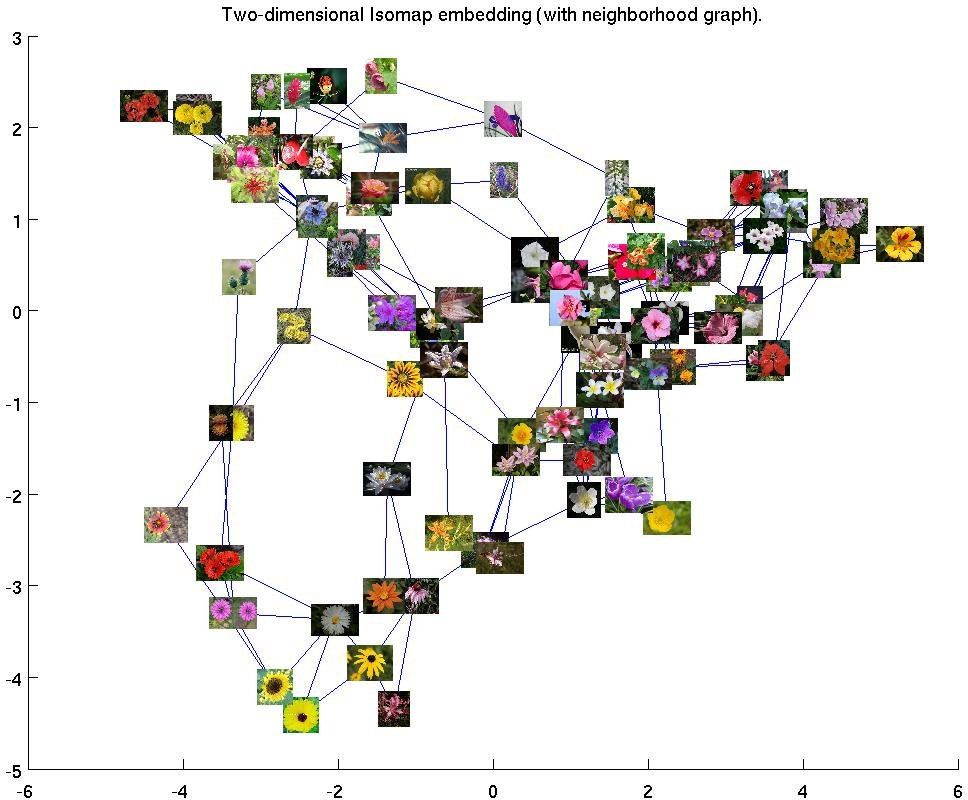
\includegraphics[height=5cm]{1.jpg}}%
  \hspace{2em}%
  \subcaptionbox{Color Isomap}
      {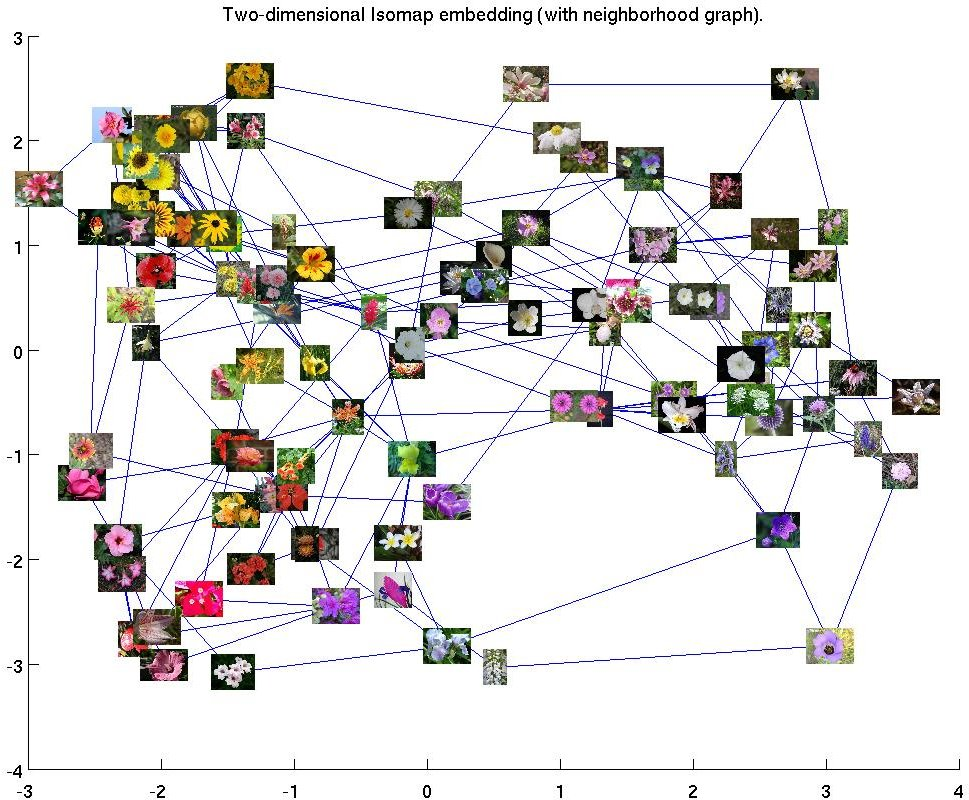
\includegraphics[height=5cm]{2.jpg}}

  \caption{Oxford 102花卉数据集的可视化}
  \end{figure}

  上述图片引用自\url{http://www.robots.ox.ac.uk/~vgg/data/flowers/102/index.html},通过SIFT特征和HSV颜色空间特征来描述花卉类别的分布。
  \subsubsection{软件需求}
  基于Python3.7.5平台编译,需要用的第三方库有:numpy、matplotlib、torch、opencv-python(3.4.2.16)、scipy等。

  \subsection{研究方案设计}
  对于一个普通的图像识别任务,通常由图像分割、特征提取和分类识别三个部分组成。图像分割是指将图像的前景或感兴趣的区域从图像中提取出来,与图像中的其他区域分割开来以屏蔽无关区域或背景对后续操作的干扰;特征提取是指运用图像处理和计算机视觉的知识对图像的特征进行合理描述,并生成可用于分类器使用的具有良好可分性的特征向量;分类识别是指将已经提取好的特征向量运用机器学习的算法对其分类,已得到分类结果,完成图像识别任务。

  花卉识别是一类典型的图像识别任务,在本次课程设计中我们同样采取上述框架,先对花卉图像进行分割取得花卉图像前景,在通过特征提取的方法获得特征向量,最后用机器学习的分类算法完成分类识别任务,具体过程如下图:\begin{figure}[H]
  \setlength{\abovecaptionskip}{0.2cm}
  \setlength{\belowcaptionskip}{-0.cm}
    \centering%
    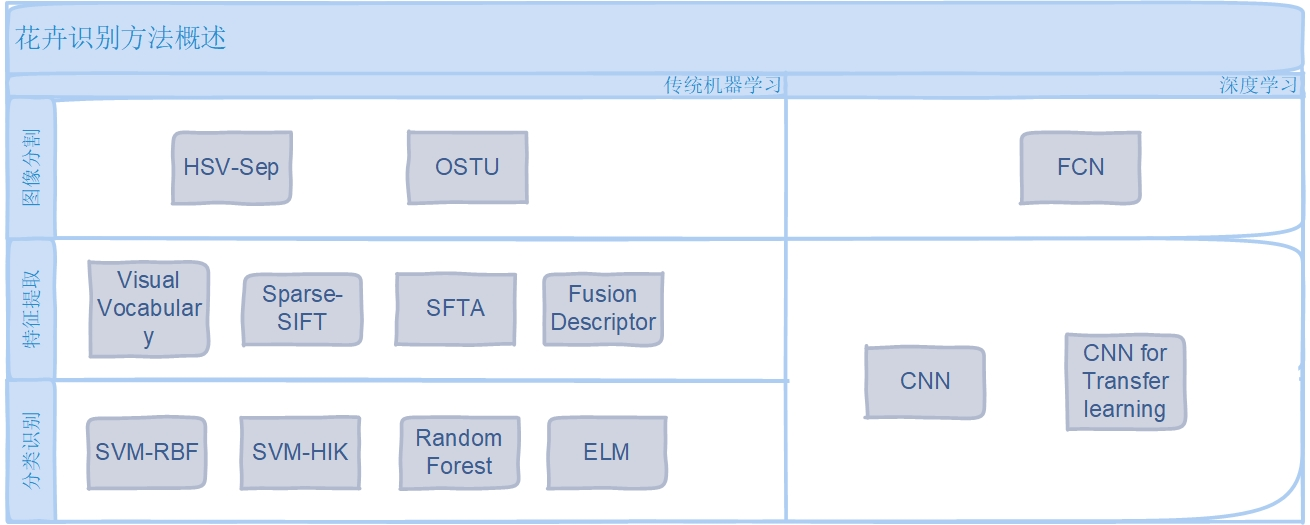
\includegraphics[scale=0.5]{3.jpg}
    \caption{花卉识别的分类框架}
  \end{figure}

  图2-2中所述的方法是本次课程设计我们所采用的方法,我们采用多种算法进行花卉识别,进行比较和分析来认识不同图像处理算法和机器学习的特性和优缺点,同时也可以通过本次课程设计拓宽知识面,增强编程和阅读文献的技能。通过阅读文献和复现文章代码,可以增进对文献中的算法的理解;通过对传统图像识别算法与深度学习进行比较可以体会到深度学习的强大性能和易用性。后面几节会逐个介绍图2-2中所介绍的方法。
  \subsection{图像分割}
  \subsubsection{基于HSV特征的图像分割方法}
  图像分割的目的是为了将花朵从背景中提取出来。可以观察到颜色的均值和标准差是一个图像的重要指标\cite{t1}。花朵图片通常包含高密度的颜色值。鲜艳的色彩吸引着鸟类和蜜蜂等授粉媒介。这样,花朵的颜色在图像中占据主导地位,平均颜色的和和颜色分布的标准差可以用来当作图像分割的阈值,具体的步骤在算法1中呈现。
  \begin{algorithm}[H] 
    \caption{基于HSV特征的图像分割} 
    \label{alg:Framwork} 
    \begin{algorithmic}[1] %这个1 表示从第一行开始显示行号,不写就不会显示行号
    \REQUIRE ~~\\ %算法的输入参数:Input
    一幅RGB图像\\
    \STATE 将RGB图像转为HSV图像;
    \STATE 计算V通道颜色特征的均值和标准差,将二者相加得到二值化的阈值;
    \STATE 将图像的V通道应用所获得的阈值二值化;
    \STATE 获得的二值化图像可能存在不连接的白色区域,选择最大的连通区域作为最后的前景区域;
    \STATE 将二值图像作为掩图应用到原有的RGB图像。
    \RETURN 分割后的RGB图像; %算法的返回值
    \end{algorithmic}
  \end{algorithm}
  需要注意的是,算法使用的V通道特征是归一化之后的特征,即将所有V通道值变为$[0,1]$。在我们实际处理花卉图片时,发现如果如上述算法所示第4步中只取最大连通区域作为前景区域,会将花的大部分区域也一同分割,我们这里将这一步忽略,虽然牺牲了一定的分割准确性,但是保留了整个花朵前景的区域。图2-3是算法的实验效果。
  \begin{figure}[H]
    \setlength{\abovecaptionskip}{0.2cm}
    \setlength{\belowcaptionskip}{-0.2cm}
    \centering%
    \subcaptionbox{原始图像} %标题的长度,超过则会换行,如下一个小图。
      {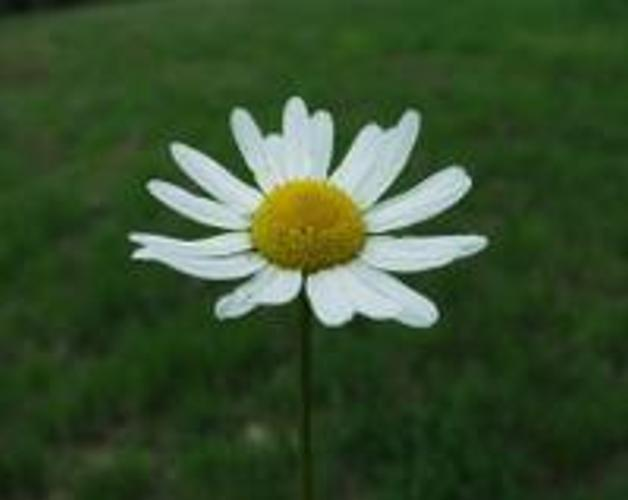
\includegraphics[height=5cm]{4.jpg}}%
    \hspace{2em}%
    \subcaptionbox{分割后的图像}
        {
\includegraphics[height=5cm]{5.jpg}}
  
    \caption{基于HSV特征的图像分割方法的实验效果}
    \end{figure}
  \subsubsection{基于OTSU的颜色分割}
  花朵的区域可以通过使用颜色特征来分割出来\cite{6968612},因为它的图像中通常包含一大片绿色的区域和花朵的区域。绿色区域代表花朵周围的叶子,花朵区域是被其颜色所特征表示的区域。

  颜色分割可以通过两种颜色的距离或差异来分割。在这个方法中,图像被转换到Lab颜色空间。然后,$\delta_E$表示每一个像素点值与平均LAB颜色的距离。在这之后,OTSU阈值被应用到L通道上完成分割。OSTU算法尝试找到一个最优的分割通过计算一个全局阈值\cite{t2}。

  图像分割问题可以看作一个二分类问题,前景是正类,而背景是负类。最佳的阈值$t^*$要能够最小化类间方差,等价于最大化类间方差。\begin{gather}
    t^*=\text{arg}\max_{1\leq t\leq L}\{ w_0(\mu_0-\mu_T)^2+w_1(\mu_0-\mu_T)^2 \}
  \end{gather}

  我们实际操作中,使用Lab空间的L通道作为分割特征,通过在计算直方图的方式将阈值在$[0,L_{\text{max}}]$找到最佳阈值。图2-4是基于OSTU的颜色分割方法的实验效果。
  \begin{figure}[H]
    \setlength{\abovecaptionskip}{0.2cm}
    \setlength{\belowcaptionskip}{-0.2cm}
    \centering%
    \subcaptionbox{原始图像} %标题的长度,超过则会换行,如下一个小图。
      {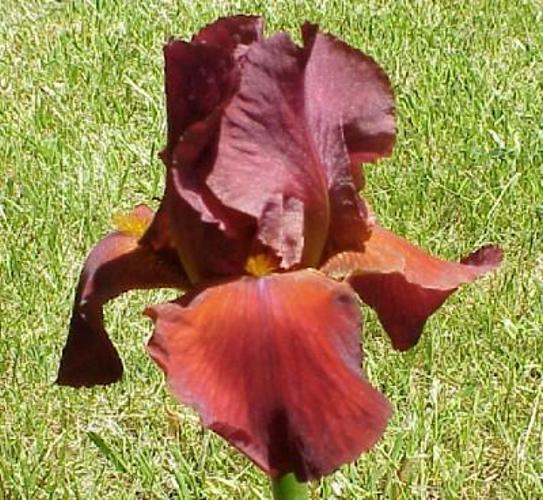
\includegraphics[height=5cm]{6.jpg}}%
    \hspace{2em}%
    \subcaptionbox{分割后的图像}
        {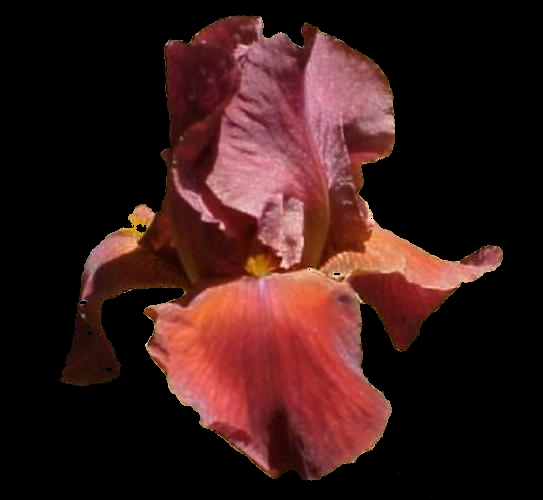
\includegraphics[height=5cm]{7.jpg}}
  
    \caption{基于OTSU的颜色分割的实验效果}
    \end{figure}
  \subsection{特征提取}
  \subsubsection{基于视觉词汇的特征提取}
  就像植物学家一样,我们为了正确区分不同类别的花朵需要能够回答特定的问题。越相似的花朵我们需要回答的问题就越多\cite{1640927}。一个花朵通常由花瓣、萼片等组成。花瓣提供了花朵种类的关键信息。一些花的花瓣有极具区分性的形状、一些可能有特殊的颜色,一些拥有辨识性的纹理模式,还有一些通过这些特性的组合而被识别。这种方法试图构建一个视觉词汇对上述三种特征给予一个正确的表示。
  \subsubsubsection{颜色词汇}
  一些花拥有很多种颜色而大多数却只有一种特殊的颜色。所以花朵的颜色特征何以帮助缩小花可能的类别。花卉图像通常是在户外情况下采集的,光照的变化对图片的影响很大。此外,花朵通常或多或少看起来有些透明,特殊强光刺激可能会导致花朵颜色变白,环境的影响因素很大。

  一种解决办法是使用一种对光照变化不敏感的颜色空间——HSV颜色空间。为了能够得到更好的泛化效果,每个像素HSV的值被提取出来用k-means方法进行聚类。
  
  给定一组聚类中心(视觉单词)$w^c_i,i=1,2,\dots,V_c$,每幅图像$I_j,j=1,2,\dots,N$,然后用一个归一化的频率直方图$n(w^c|I_j)$表示。一幅新的图像可以基于频率直方图特征的最近邻分类器。\begin{gather}
    c^*=\text{arg}\min_j d(n(w^c|I^{\text{test}}),n(w^c|I^{\text{train}}_j))
  \end{gather}
  其中距离$d(.)$使用$\chi^2$度量。实际使用过程中,我们发现对每幅图像的所有像素点进行聚类速度太慢,所以我们实际操作中采用下面的方法加速计算。

  对于一幅给定的HSV图像$I$,对于每一行和每一列像素,分别计算当前行/列的均值向量$\bm{m}$和协方差矩阵$\Sigma$,将协方差矩阵铺平成一维向量,再与均值向量拼接成一个向量$\bm{v_i}$作为一行/列特征,每幅图像以这个计算得的向量做聚类操作,完成上述后续操作。

  图2-5所示是上述方法的图示解释,实践中我们发现,因为原有特征提取的耗时性只要来源于对每幅图像的每个像素进行k-means聚类。举个例子,对于一幅500*600大小的图像,就有300000个像素点进行聚类,这个对k-means是极其耗时且复杂的,运用我们方法,同样也可以表示颜色特征,但数据点样本只有1100个,k-means的速度大大提升,使在我们的硬件平台上可以完成实验并得到结果。
  \begin{figure}[H]
    \setlength{\abovecaptionskip}{0.2cm}
    \setlength{\belowcaptionskip}{-0.cm}
      \centering%
      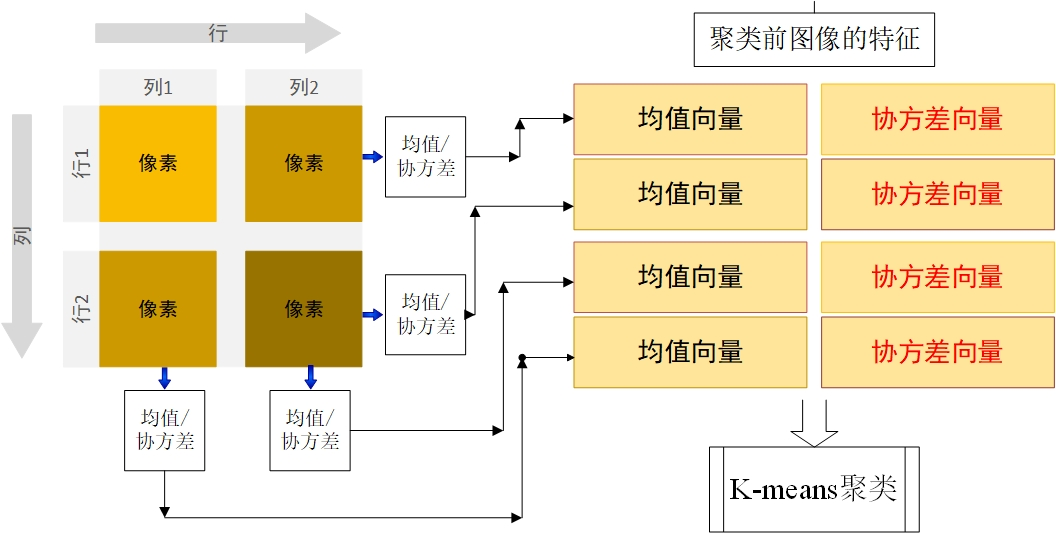
\includegraphics[scale=0.5]{8.jpg}
      \caption{提取颜色词汇特征的框架}
    \end{figure}
  \subsubsubsection{形状词汇和纹理词汇}
  每一朵花的花瓣的形状、构造和全局形状可以被用来区分花卉种类。视角和清晰度的变化改变了花卉的形状,所以自然界的自然形变极大提升分类问题的难度。所以我们想到采用SIFT特征描述子对每一幅图像提取特征点和相关特征。我们使用与2.4.1.1中相同的视觉特征提取方法和分类方法\footnote{这里直接提取SIFT特征而不用求行/列均值和方差。}获得形状词汇特征$n(w^s|I)$,用于后续分类,分类的方法与2.4.1.1所述的一致。

  一些花朵的花瓣存在特定的纹理模式,他们更具有区分性,原文\cite{1640927}中采用的是MR8滤波器组来提取纹理特征,我们实验中发现MR8滤波器组提取特征时十分耗时,所以这里我们采用LBP算子提取纹理特征,对于LBP算子处理过后的灰度图像应用与提取颜色词汇特征同样的步骤,包括求行/列均值和方差简化计算来得到纹理词汇的描述$n(w^t|I)$。分类的方法与之前提到的颜色词汇和形状词汇一样\footnote{关于SIFT特征描述子和LBP算子的介绍见附录A。}。
  \subsubsubsection{组合词汇}
  为了将三种特征词汇很好地结合起来,我们引入了一组权重向量$\bm{\alpha}$,所以我们最终得到的特征直方图如式(2.3)所示。\begin{gather}
  n(w|I)=\begin{bmatrix}
    \alpha_sn(w^s|I)\\
    \alpha_cn(w^c|I)\\
    \alpha_tn(w^t|I)
  \end{bmatrix}
  \end{gather}
  这种将对于每个方面的分类的结合与组合独立的分类器相似。$\bm{\alpha}$权重向量给了关于距离向量的线性组合。为了更明白的说明这个问题,在这种情况下,$d(\alpha\bm{x},\alpha\bm{y})=\alpha d(\bm{x},\bm{y})$,所以最终的分类问题如式(2.4)描述。\begin{gather}
  \begin{array}{ll}
   c^*=\text{arg}\min_j\{ & \alpha_sd(n(w^s|I^{\text{test}}),n(w^s|I_j^{\text{train}}))+\\
   &\alpha_cd(n(w^c|I^{\text{test}}),n(w^c|I_j^{\text{train}}))+\\
   &\alpha_td(n(w^t|I^{\text{test}}),n(w^t|I_j^{\text{train}})) \}
  \end{array}
  \end{gather}
  \subsubsection{基于融合特征描述子的特征提取}
  W. Liu等人在\cite{8090865}中提出了一种基于DenSIFT的直方图特征和LLC稀疏编码的特征提取方法,图2-6展示了该方法的流程。
  \begin{figure}[H]
    \setlength{\abovecaptionskip}{0.2cm}
    \setlength{\belowcaptionskip}{-0.cm}
      \centering%
      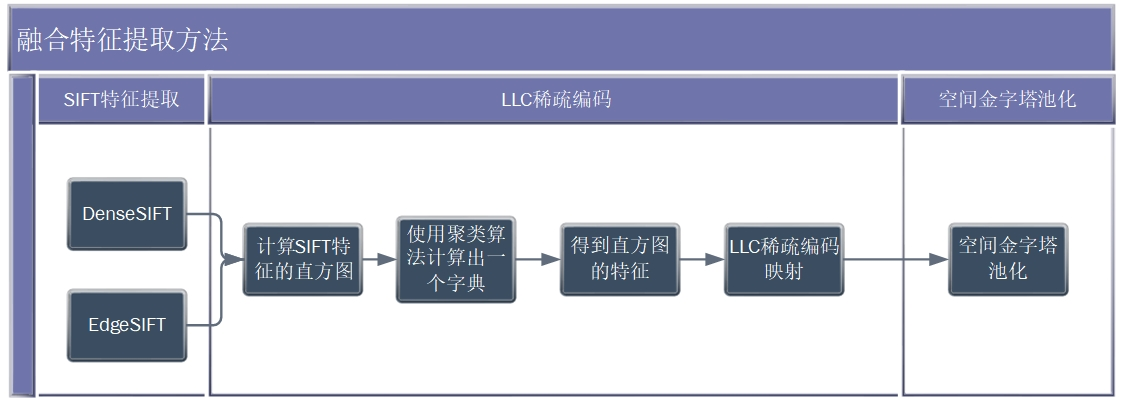
\includegraphics[scale=0.6]{9.jpg}
      \caption{基于融合特征描述子的特征提取流程}
    \end{figure}

  颜色和纹理特征是在花卉识别的领域的两个重要且具有区分性的特征。将二者合理地结合可以很大幅度提高分类算法的性能。在这里,我们使用PHOW-Color、PHOW-Gray和edge-SIFT来提取花卉特征。

  PHOW(a Pyramid Histogram Of visual Words)是一种基于bad-of-words方法改进的特征表示方法,通过提取多尺度的Dense SIFT来保持特征信息的空间分布。主要有两个不同版本的PHOW,分别应用于颜色和纹理的特征提取上。PHOW-Color被用于分别提取图像的H、S、V三个通道上的PHOW特征,然后将它们拼接成一个完整的特征。PHOW-Gray是另一种PHOW模型用于在灰度空间上提取图像特征。

  PHOW的提取过程主要有散步:Dense-SIFT特征提取、建立视觉词典和空间金字塔池化。其中建立视觉字典的过程与2.4.1.1中建立字典的过程一致,这里不再赘述。
  \subsubsubsection{Dense SIFT和Edge SIFT特征提取}
  Dense SIFT是SIFT特征的一种改进型,首先将表达目标的矩形区域分成相同大小的矩形块,计算每一个小块的SIFT特征,再对各个小块的稠密SIFT特征在中心位置进行采样,建模对目标的表达。在这里,我们在以$16\times16$的像素为大小、以8个像素为步长的网格划分出的区域上计算Dense SIFT特征。这样,我们可以得到一个在颜色和纹理层次上SIFT特征描述:\begin{gather}
     S^i=\{ (d_1,k_1),(d_2,k_2),\cdots,(d_S,k_S) \}\text{  }i\in(0,1)
  \end{gather}
  上式中$S^i$在$i=0$时表示提取的是颜色特征,而$i=1$是表示提取的是纹理特征,$d_i$表示在其对应的几何坐标系下的$d$维的SIFT特征向量,$k_i$表示第$i$个描述子的几何坐标系。$S$表示网格区域的个数。

  通过统计的方法得到这些描述子的直方图,即\begin{gather}
     H_i=\{h_1,h_2,\cdots,h_n\}
  \end{gather}
  其中$n$是直方图的维度。

  Edge SIFT被用来提取一幅轮廓图像的SIFT特征来表示图像的形状特征。在这里,我们通过Canny算子\footnote{关于Canny算子的介绍见附录A}得到一幅图像的轮廓图。也就是说,对于一幅图像$I$,其轮廓图像$C$为二值化图像,即\begin{gather}
    C(i,j)=\left\{
    \begin{array}{ll}
     1&\text{if }I(i,j)\text{is contours}\\
     0&\text{if }I(i,j)\text{is not contours}
    \end{array}
    \right.
  \end{gather}
  
  应用与上述一样的方法得到Edge SIFT描述子的直方图。
  \subsubsubsection{Locality-constrained Linear Coding}
  这里我们采用Locality-constrained Linear Coding(LLC)编码方式来对提取出的直方图字典特征进行编码。这种编码方式更多的考虑局部信息,认为局部信息比稀疏性更重要。LLC采用了局部约束取代了其他编码方式中采用的稀疏约束\cite{5540018}。
  
  假定我们已经得到了每幅图像的特征的统计直方图。令$D$表示每个直方图的维度,K-Means学习得到的字典$B=\{ b_1,b_2,\cdots,b_m \}\in\mathbb{R}^{D\times M}(M\gg D)$,$M$表示聚类中心的个数。令$I=\{ I_1,I_2,\cdots,I_N \}\in\mathbb{R}^{D\times N}$代表一个从图像中提取的$D$维的局部特征。LLC试图在$B$中通过欧氏距离度量找到$k$个最近邻来构建一个小字典$\tilde{B}=\{ b_{[1]},b_{[2]},\cdots,b_{[k]} \}\in\mathbb{R}^{D\times k}$,这里$k$是用户指定的超参数。即\begin{gather}
  \begin{array}{ll}
  \min\limits_C&\sum\limits^N_{i=1}\lVert x_i-Bc_i\rVert^2+\lambda\lVert d_i\odot c_i\rVert^2\\
  s.t.&\mathbf{1}^Tc_i=1,\forall i
  \end{array}
  \end{gather}
  这里$\odot$表示矩阵对应元素相乘,$d_i\in\mathbb{R}^M$表示位置适配器,根据与输入特征$x_i$的相似程度给每个基向量赋予不同的自由度。具体来说,\begin{gather}
     d_i=\exp\left( \dfrac{\text{dist}(x_i,B)}{\sigma} \right)
  \end{gather}
  这里$\text{dist}(x_i,B)=[\text{dist}(x_i,b_1),\dots,\text{dist}(x_i,b_M)]^T$,$\text{dist}(x_i,b_j)$表示$x_i$和$b_j$的欧氏距离。$\sigma$用于调整局部适配器的权重衰减。在计算时要对$d_i$进行归一化。图2-7所示是LLC编码的过程。
  \begin{figure}[H]
    \setlength{\abovecaptionskip}{0.2cm}
    \setlength{\belowcaptionskip}{-0.cm}
      \centering%
      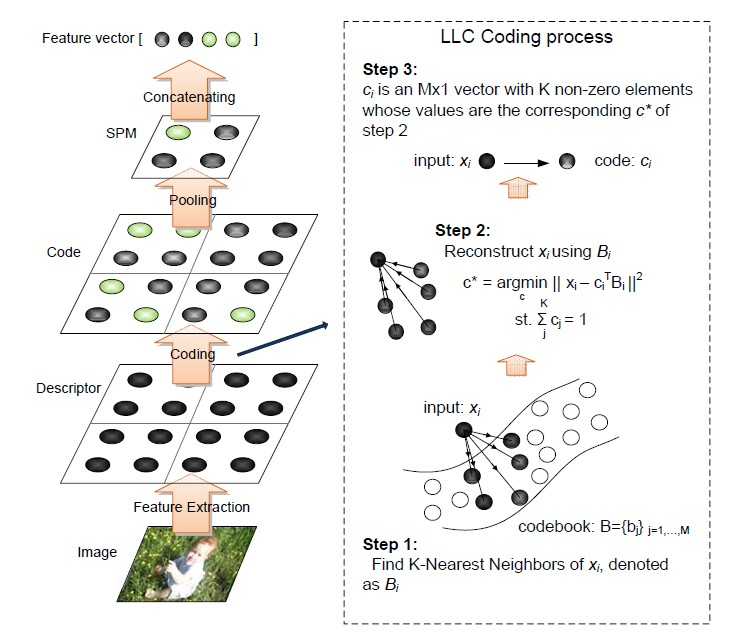
\includegraphics[scale=0.8]{11.jpg}
      \caption{LLC编码流程}
    \end{figure}
  式(2.8)所示的优化问题一个很好的性质是拥有解析解,可以避免迭代求解造成的大量计算资源和时间的消耗。LLC的解析解形式如式(2.11)所示。\begin{gather}
   \tilde{c}_i=(C_i+\lambda\text{diag}(d))\setminus\mathbf{1}\\
   c_i=\tilde{c}_i/\mathbf{1}^T\tilde{c}_i
  \end{gather}
  这里$C_i=(B-\mathbf{1}x_i^T)(B-\mathbf{1}x_i^T)^T$是数据的协方差矩阵。
  \subsubsubsection{空间金字塔池化}
  空间金字塔表示(Spatial Pyramid Representation, SPR)是一种当下十分流形的特征编码方式。如图2-8中所示,在每一个金字塔等级$l$下,输入图像被分为一系列递增的重叠网格。所有的描述子都从每一个网格中提取特征,然后拼合成最终的图像特征描述。
  \begin{figure}[H]
    \setlength{\abovecaptionskip}{0.2cm}
    \setlength{\belowcaptionskip}{-0.cm}
      \centering%
      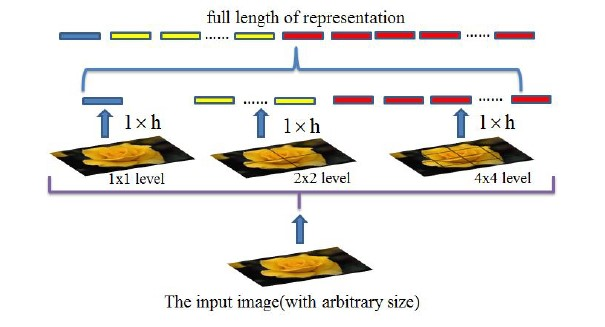
\includegraphics[scale=0.8]{10.jpg}
      \caption{空间金字塔池化示意图}
    \end{figure}
  
  在这里我们采用LLC(Locality-constrained Linear Coding)体系来对每个网格提取的特征进行编码,每个局部字典大小设为60.我们建立了一个3层金字塔,包括$1\times1$、$2\times2$和$4\times4$不同的子区域。令$h^j_{C(l)}\in \mathbb{R}^d$表示从第$j$层的网格$C(l)$上提取的PHOW特征编码。所以,最终图像$I_i$的PHOW特征编码表示为\begin{gather}
   H^k_i=\{ h^0_1,h^1_1,\cdots,h^l_{C(l)} \}
  \end{gather}
  这里,当$k=1$时表示在HSV空间上提取的PHOW特征,$k=0$时表示在灰度空间上提取的PHOW特征,$k=2$时表示提取的Edge SIFT特征。
  \subsubsection{基于稀疏编码的SIFT特征}
  SIFT(Scale Invariant Feature Transform)特征描述子是一种被广泛应用于图像和计算机视觉领域来提取特征点,对光照、尺度和旋转具有一定的不变性,可以用来提取花卉分类的特征。Hossam M.Z.在\cite{6968612}中将SIFT特征提取出来的结果采用稀疏编码的方式得到图像的特征。

  在我们具体实践的时候,我们采用了DenseSIFT描述子来提取图像的特征,最后在采用式(2.13)进行稀疏编码。\begin{gather}
   \min\text{  }\sum\limits^N_{i=1}\left( \left\lVert x_i-\sum\limits^M_{j=1} a_i^{(j)}\phi^{(j)} \right\rVert^2+L \right)\\
   L=\lambda\sum\limits^M_{j=1}\left\lvert a_i^{(j)} \right\rvert
  \end{gather}
  其中$x_i$是SIFT提取的特征,$a^j$中大部分元素都是零,$\phi$是稀疏编码的基,$\lambda$是权重向量。我们在实际过程中采用KSVD算法求解稀疏编码问题\cite{CHENG2014416}。
  \begin{algorithm}[H] 
    \caption{K-SVD稀疏编码} 
    \label{alg:Framwork} 
    \begin{algorithmic}[1] %这个1 表示从第一行开始显示行号,不写就不会显示行号
    \REQUIRE  原始样本、字典、稀疏矩阵\\
    \ENSURE  字典、稀疏矩阵\\
    \STATE \textbf{初始化}:从原始样本$Y\in\mathbb{R}^{m\times n}$随机取$K$个列向量或者取它的左奇异矩阵的前$K$个列向量$\{ d_1,d_2,\cdots,d_K \}$作为初始字典的原子,得到字典$D^{(0)}\in\mathbb{R}^{m\times K}$。令$j=0$,重复下面的步骤,直到达到指定的迭代步数,或收敛到指定的误差:
    \STATE  \textbf{稀疏编码}:利用字典上一步得到的字典$D^{(j)}$,稀疏编码,得到$X^{(j)}\in\mathbb{R}^{K\times n}$;
    \STATE  \textbf{字典更新}:逐列更新字典$D^{(j)}$,字典的列$d_k\in\{ d_1,d_2,\cdots,d_K \}$;
    \STATE  当更新$d_k$时,计算误差矩阵$E_k=Y-\sum_{j\neq k}d_jx^j_T$;
    \STATE  取出稀疏矩阵第$k$个行向量$x^k_T$不为0的索引的集合$w_k=\{ i|1\leq i\leq n,x^k_T(i)\neq 0 \}$,$x^{'k}_T=\{ x^k_T(i)|1\leq i\leq n,x^k_T(i)\neq 0 \}$;
    \STATE 从$E_k$取出对应$w_k$不为0的列,得到$E^{'}_{k}$;
    \STATE 对$E^{'}_{k}$作奇异值分解$E_k=U\Sigma V^T$,取$U$的第1列更新字典的第$k$列,即$d_k=U(\cdot,1)$,令$x^{'k}_T=\Sigma(1,1)V(\cdot,1)^T$,得到$x^{'k}_T$后,将其对应地更新到原$x^k_T$;
    \STATE $j=j+1$
    \end{algorithmic}
  \end{algorithm}
  \subsubsection{基于分割的分形纹理分析}
  基于分割的分形纹理分析(Segmentation-based Fractal Texture Analysis, SFTA)主要分为两个部分\cite{6382737}:1)把输入的灰度图像分解成一系列二值图像,这里采用两阈值二值化分解(Two-Threshold Binary Decomposition, TTBD)进行二值化;2)对于上述得到的二值化图像,我们计算区域的边界的分形维度,另外在计算区域的平均灰度值和面积。
  \subsubsubsection{两阈值二值化分解}
  两阈值二值化分解(TTBD)将一幅灰度图像$I(x,y)$当作输入,并且返回一系列二值图像。两阈值二值化分解的第一步是计算一组分割阈值$T$。两阈值二值化分解采用一种叫做多等级OTSU(multi-level OTSU)算法,利用输入图像的灰度分布信息来计算阈值。

  多等级OTSU算法的步骤如下:寻找到阈值能够使输入的图像的类内方差最小化;然后,以递归的方式不断对每一幅输入图像区域应用OSTU算法直到得到$n_t$个阈值,这里$n_t$是一个预先设定的参数。图2-9所示是两阈值二值化分解的工作流程。
  \begin{figure}[H]
    \setlength{\abovecaptionskip}{0.2cm}
    \setlength{\belowcaptionskip}{-0.cm}
      \centering%
      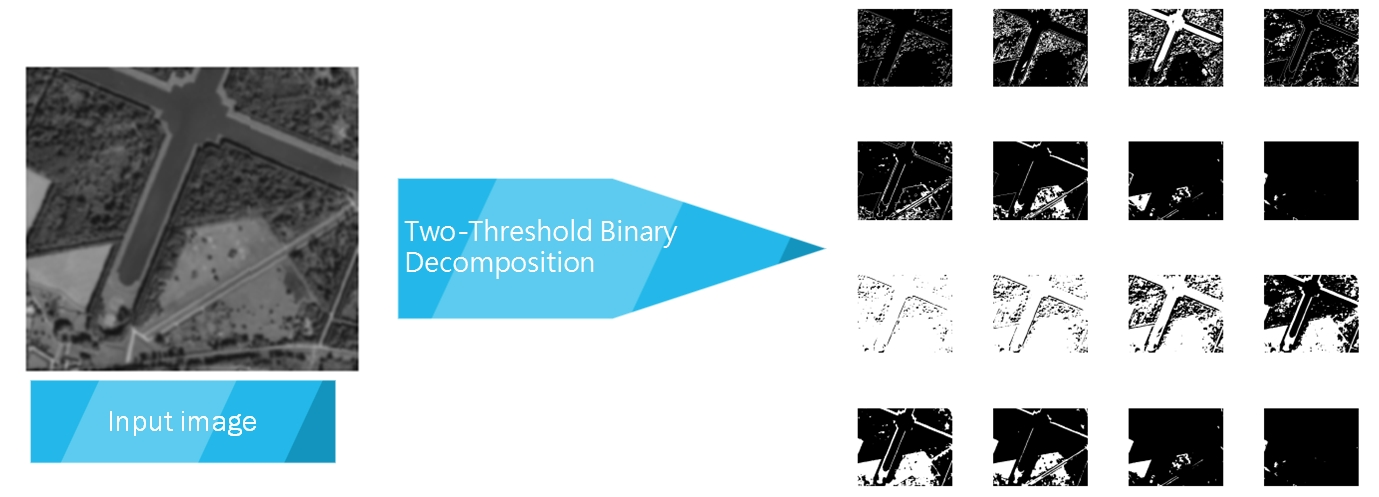
\includegraphics[scale=0.5]{12.jpg}
      \caption{两阈值二值化分解的示意图}
    \end{figure}
  
  接下来,利用得到的阈值将输入灰度图像$I(x,y)$分解成一系列二值图像,即\begin{gather}
   I_b(x,y)=\left\{
    \begin{array}{ll}
       1&\text{if }t_l<I(x,y)\leq t_u\\
       0&\text{otherwise}
    \end{array}
   \right.
  \end{gather}
  这里$t_l$和$t_u$是用于分割的上界和下界。

  给定一幅输入图像,使用从$T\cup\{ n_l \}$得到的所有邻近的阈值对和从$\{ t,n_l \},t\in T$得到的所有邻近的阈值对,通过式(2.15)可以得到一系列二值图像,$n_l$代表$I(x,y)$的最大可能出现的灰度值。这样一幅输入的灰度图像可以得到$2n_t$个二值图像。

  两阈值二值化分解的一个重要性质是,所得的二值图像是通过使用多级OTSU算法计算的阈值应用单阈值分割而获得的所有二值图像的超集合。

  使用阈值对分割得到二值图像的基本原理是对那些常规阈值分割无法分割出的图像进行分割,尤其是那些目标的灰度区域在输入图像灰度直方图的中部范围。通过使用阈值对可以将那些中等亮度的目标的区域信息从原图像中提取出来。
  \subsubsubsection{SFTA特征提取}
  在对输入灰度图像进行两阈值二值分解之后,将二值图像的面积、平均灰度值和边界分形维度组成最后SFTA的特征向量。分形度量被用来表示分割后的目标和结构的边界复杂度。二值图像$I_b(x,y)$的边界组成一幅边界图像记作$\Delta(x,y)$,有\begin{gather}
   \Delta(x,y)=\left\{
    \begin{array}{lll}
      1&\text{if}&\exists(x^{'},y^{'})\in N_8[(x,y)]:\\
       &         &I_b(x^{'},y^{'})=0\land\\
       &         &I_b(x,y)=1,\\
      0&\text{otherwise.}&
    \end{array}
   \right.
  \end{gather}
  这里$N_8[(x,y)]$是该像素的8-邻域。通过式(2.16)得到的边界是一像素宽的。再在每一个得到的边界图像上计算分形维数$D$。

  分形几何包括多种定义分形维数的方法,这里我们采用的最为常见的Hausdorff维度。考虑一个目标的欧式维度是$E$,它的Hausdorff分形维度$D_0$可以由式(2.17)计算得到\begin{gather}
   D_0=\lim_{\epsilon\to 0}\dfrac{\log N(\epsilon)}{\log \epsilon^{-1}}
  \end{gather}
  这里$N(\epsilon)$是$E$维的超立方体的个数,$\epsilon$表示填充目标的长度。

  如果我们考虑一个由二值图像$I_b$表示的目标,可以通过Box Counting算法计算$D_0$的近似$D$。不失一般性,下面我们考虑2D的情形。起初,图像被分为一个由$\epsilon\times\epsilon$的方格组成的网格。接下来再每一个方格中输出至少包含一个目标像素的$\bar{N}(\epsilon)$。通过改变$\epsilon$的值,可以得到一条$\log\bar{N}(\epsilon)$-$\log\epsilon^{-1}$曲线。最终,通过线拟合方法,用一条直线近似这条曲线,最后分形维数$D$就是这条直线的斜率。

  平均灰度值和区域面积用来补充从每一张二值图像提取出来的信息,同时不显著增加计算负担。这样,SFTA特征向量的维度等于两阈值二值化分解得到的图像个数的三倍:分形维度、平均灰度值和区域面积。图2-10说明从每幅二值图像提取出来的三个特征。
  \begin{figure}[H]
    \setlength{\abovecaptionskip}{0.2cm}
    \setlength{\belowcaptionskip}{-0.cm}
      \centering%
      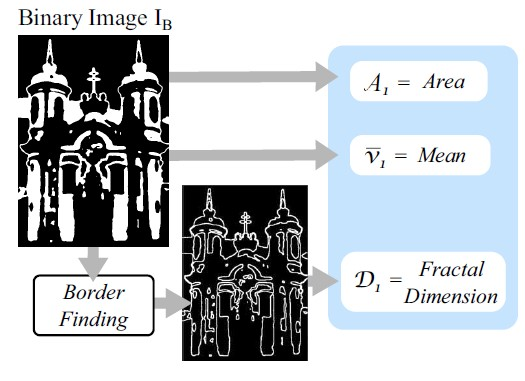
\includegraphics[scale=0.8]{13.jpg}
      \caption{SFTA特征向量的组成}
    \end{figure}
  \begin{algorithm}[H] 
    \caption{SFTA特征提取} 
    \label{alg:Framwork} 
    \begin{algorithmic}[1] %这个1 表示从第一行开始显示行号,不写就不会显示行号
    \REQUIRE  灰度图像$I$,阈值的个数$n_t$\\
    \ENSURE  特征向量$V_{\text{SFTA}}$\\
    \STATE $T\leftarrow \mathbf{MultiLevelOTSU}(I,n_t)$
    \STATE $T_A\leftarrow \{ \{ t_i,t_{i+1} \}:t_i,t_{i+1}\in T,i\in [1\dot\dot|T|-1] \}$
    \STATE $T_B\leftarrow \{ \{ t_i,n_l\}:t_i\in T,i\in [1\dot\dot |T|] \}$
    \STATE $i\leftarrow 0$
    \FOR{$\{ \{ t_l,t_u \}:\{ t_l,t_u \}\in T_A\cup T_B \}$} 
    \STATE  $I_b\leftarrow\mathbf{TwoThresholdSegmentation}(I,t_l,t_u)$
    \STATE  $\Delta(x,y)\leftarrow\mathbf{FindBorders}(I_b)$
    \STATE  $V_{\text{SFTA}}[i]\leftarrow\mathbf{BoxCounting}(\Delta)$
    \STATE  $V_{\text{SFTA}}[i+1]\leftarrow\mathbf{MeanGrayLevel}(I,I_b)$
    \STATE  $V_{\text{SFTA}}[i+2]\leftarrow\mathbf{PixelCount}(I_b)$
    \ENDFOR
    \RETURN $V_{\text{SFTA}}$
    \end{algorithmic}
  \end{algorithm}

  算法3说明了SFTA特征提取的过程。$V_{\text{SFTA}}$表示最后得到的特征向量。第1行表示通过多级OSTU算法计算一系列的阈值;第2行将$T$所有邻近的阈值对加入$T_A$;第3行将阈值对$\{ t_i,n_l \}$加入到$T_B$中;第5行将所有阈值对组合,即$T_A\cup T_B$;第6行使用每一个阈值对分割图像;7-10行计算分型维度、平均灰度值和区域面积。
  \subsection{机器学习分类算法}
  \subsubsection{支持向量机}
  支持向量机(Support Vector Machine, SVM)是机器学习中最为流行的分类算法之一。以二分类问题为例,给定训练数据$(\bm{x}_i,t_i),i=1,\dots,N$,这里$\bm{x}_i\in\mathbb{R}^d$和$t_i\in\{ -1,1 \}$,由于一般情况下,数据通常线性不可分,所以通常将原始训练数据$\bm{x}_i$通过非线性映射映射到一个新的特征空间$Z$:$\phi:\bm{x}_i\to\phi(\bm{x}_i)$。再新的特征空间$Z$中不同的类之间的距离为$2/\lVert \bm{w} \rVert$。为了同时最大化类间距离和最小化训练误差$\xi_i$,等价于\begin{gather}
  \begin{array}{ll}
  \text{Minimize}&L_{P_{\text{SVM}}}=\dfrac{1}{2}\lVert \bm{w} \rVert^2+C\sum\limits^N_{i=1}\xi_i\\
  \text{Subject to}&t_i(\bm{w}\phi(\bm{x}_i)+b)\geq 1-\xi_i,\text{ }i=1,\dots,N\\
                 &\xi_i\geq 0,\text{ }i=1,\dots,N
  \end{array}
  \end{gather}
  $C$是一个超参数用于平衡分类间隔和训练误差。

  基于Karush-Kuhn-Tucker(KKT)定理,训练上述的支持向量机等价于求解下面的对偶优化问题:\begin{gather}
   \begin{array}{ll}
   \text{minimize}&L_{D_{\text{SVM}}}=\dfrac{1}{2}\sum\limits^N_{i=1}\sum\limits^N_{j=1}t_it_j\alpha_i\alpha_j\phi(\bm{x}_i)\phi(\bm{x}_j)-\sum\limits^N_{i=1}\alpha_i\\
   \text{subject to}&\sum^N_{i=1}t_i\alpha_i=0\\
                    &0\leq\alpha_i\leq C,\text{ }i=1,\dots,N
   \end{array}
  \end{gather}
  这里拉格朗日系数$\alpha_i$对应于训练样本$(\bm{x}_i,t_i)$。对于向量$\bm{x}_i$,若满足$t_i(\bm{w}\phi(\bm{x}_i)+b)=1$则$\bm{x}_i$为支撑向量。

  核函数是支撑向量机的一大技巧。令核函数为$K(\bm{u},\bm{v})=\phi(\bm{u})\phi(\bm{v})$,这样有\begin{gather}
  \begin{array}{ll}
  \text{minimize}&L_{D_{\text{SVM}}}=\dfrac{1}{2}\sum\limits^N_{i=1}\sum\limits^N_{j=1}t_it_j\alpha_i\alpha_jK(\bm{x}_i,\bm{x}_j)-\sum\limits^N_{i=1}\alpha_i\\
  \text{subject to}&\sum\limits^N_{i=1}t_i\alpha_i=0\\
                   &0\leq\alpha_i\leq C,\text{ }i=1,\dots,N
  \end{array}
  \end{gather}
  
  最后支持向量机的决策函数为\begin{gather}
  f(\bm{x})=\text{sign}\left( \sum\limits^{N_s}_{s=1}\alpha_st_sK(\bm{x},\bm{x}_s)+b \right)
  \end{gather}
  这里$N_s$是支撑向量的个数。

  本次课程设计中,除了采用常用的RBF核,我们采用了一种叫直方图交叉核(Histogram Intersection Kernel, HIK)的核函数\cite{5459178}。令$\bm{h}=(h_1,\dots,h_d)\in\mathbb{R}^d_+$为一个直方图,$\bm{h}$能够代表一幅图像或一个子区域。定义直方图交叉核$\mathcal{K}_{\text{HI}}$为\begin{gather}
   \mathcal{K}_{\text{HI}}(\bm{h}_1,\bm{h}_2)=\sum\limits^d_{i=1}\min(h_{1i},h_{2i})
  \end{gather}
  可以证明$\mathcal{K}_{\text{HI}}$是一个有效的正定核函数。这样存在一个映射$\phi$将任何一个直方图$\bm{h}$映射到对应的高维空间$\Phi$的向量$\phi(\bm{h})$,即$\mathcal{K}_{\text{HI}}(\bm{h}_1,\bm{h}_2)=\phi(\bm{h}_1)\phi(\bm{h}_2)$。通过非线性映射$\phi$,直方图的相似性等价于在高维空间$\Phi$的内积。
  \subsubsection{随机森林}
  随机森林(Random Forest, RF)是一系列树结构的分类器的集成。每一棵树依赖于一个独立采样的随机向量和森林中全部的树的分布。它本质上是决策树(Decision Tree, DT)的集成。主要的原理是通过将多个弱分类器集成来建立一个强分类器。

  随机森林分类器从树的顶部开始输入,指导最后到达一个叶子节点。原始数据被随机采样,但是不断替换成更小的集合。采样样本的类别由随机森林的树决定,这里是个任意数。

  令$(X_1,Y_1),(X_2,Y_2),\dots,(X_n,Y_n)$是随机变量对,其中$X\in\mathbb{R}^d$是特征向量,$Y\in\{ 0,1 \}$是由随机变量产生的标签集。$(X,Y)$的联合分布由$X$的边际分布$\mu$(即,$P\{ X\in A \}=\mu(A)$对于集合$A\subset \mathbb{R}^d$),和一个后验概率$\eta:\mathbb{R}^d\to[0,1]$,\begin{gather}
   \eta(x)=p(Y=1|X=x)
  \end{gather}

  $D_n$表示训练数据,为$(X_1,Y_1),(X_2,Y_2),\dot,(X_n,Y_n)$的集合。一个分类器$g_n$是一个关于$X$和$D_n$的二值函数,其错误概率为\begin{gather}
   L(g_n)=P_{(x,y),z}\{ g_n(X,D_n)\neq Y \}
  \end{gather}

  这里$P_{(x,y)}$表示关于$(X,Y)$的概率,也即是由$D_n$的条件概率。随机森林是平均分类器。正式地说,一个有$m$颗树的随机森林是一个基于随机化产生的树分类器$g_n(x,Z_1),\dots,g_n(x,Z_m)$的集合。$Z_1,\dots,Z_m$是同分布的随机向量,在$X,Y,D_n$上条件独立。随机变量通常用于确定在构建树时如何执行连续剪切,例如选择节点和要拆分的坐标以及拆分的位置。

  随机森林在以决策树为基学习器构建Bagging集成的基础上,进一步在决策树的训练过程中引入了随机属性选择。具体地说,传统决策树在选择划分属性时是在当前结点的属性集合(假定有$d$个属性)中选择一个最优属性;而在随机森林中,对基决策树的每个结点,先从该点的属性集合中随机选择一个包含$k$个属性的子集,然后再从这个子集中选择一个最优属性用于划分。这里的参数$k$控制了随机性的引入程度:若令$k=d$,则基决策树的构建与传统决策树相同;若令$k=1$,则是随机选择一个属性用于划分;一般情况下,推荐值$k=\log_2d$。随机森林中基学习器的多样性不仅来自样本扰动,还来自属性扰动,这就使得最终集成的泛化性能可通过个体学习器之间差异度的增加而进一步提升。
  \subsubsection{极限学习机}
  极限学习机(Extreme Learning Machine, ELM)是单隐层前馈神经网络,随机确定输入权重和可以通过解析解得到输出权重参数\cite{1380068}。首先我们要介绍一种Moore-Penrose广义逆矩阵和一个一般线性系统$\bm{Ax}=\bm{y}$的最小范数最小二乘解,其次介绍极限学习机的基本流程。
  \subsubsubsection{Moore-Penrose广义逆矩阵}
  广义线性系统$\bm{Ax}=\bm{y}$的解,这里$\bm{A}$可能是奇异的,也可能不是方阵,这时需要用Moore-Penrose广义逆矩阵求解。
  \begin{definition}
  \textbf{Moore-Penrose广义逆矩阵:}一个矩阵$G\in\mathbb{R}^{n\times m}$是$A\in\mathbb{R}^{m\times n}$的Moore-Penrose广义逆矩阵,当且仅当\begin{gather}
    AGA=A,GAG=G,(AG)^T=AG,(GA)^T=GA
  \end{gather}
  \end{definition}
  为了简化表示,记矩阵$A$的Moore-Penrose广义逆矩阵为$A^{\dag}$。
  \subsubsubsection{一般线性系统的最小范数最小二乘解}
  对于一个一般的线性系统$\bm{AX}=\bm{y}$,我们称$\hat{\bm{x}}$是一个最小二乘解,当且仅当\begin{gather}
     \lVert \bm{A\hat{x}}-\bm{y} \rVert=\min\limits_{\bm{x}}\lVert \bm{Ax-y} \rVert
  \end{gather}
  这里$\lVert\cdot\rVert$是欧式空间的范数。
  \begin{definition}
  $\bm{x}_0\in\mathbb{R}^n$被称为线性系统$\bm{Ax=y}$最小范数最小二乘解如果对任意$\bm{y}\in\mathbb{R}^m$有\begin{gather}
   \lVert \bm{x}_0 \rVert,\forall \bm{x}\in\{ \bm{x}:\lVert \bm{Ax-y} \rVert\leq\lVert \bm{Az-y} \rVert,\forall\bm{z}\in\mathbb{R}^n \}
  \end{gather}
  \end{definition}
  也就是说,一个线性系统$\bm{Ax=y}$的最小范数最小二乘解$\bm{x}_0$如果它是所有最小二乘解中范数最小的解。
  \begin{theorem}
   假设存在矩阵$\bm{G}$使得$\bm{Gy}$是线性系统$\bm{Ax=y}$的最小范数最小二乘解,当且仅当$\bm{G}=\bm{A}^{\dag}$。
  \end{theorem}
  也就是说$\bm{G}$是$\bm{A}$的Moore-Penrose广义逆矩阵。
  \subsubsubsection{极限学习机的基本原理}
  对于$N$个可分样本$(\bm{x}_i,\bm{t}_i)$,这里$\bm{x}_i=[x_{i1},x_{i2},\cdots,x_{in}]^T\in\mathbb{R}^n$,$\bm{t}_i=[t_{i1},t_{i2},\cdots,t_{im}]^T$ $\in\mathbb{R}^m$,标准的有$\bar{N}$个隐层神经元和激活函数$g(x)$的单隐层前馈神经网络(Single hidden Layer Feedforward Networks, SLFNs),即\begin{gather}
    \sum\limits^{\bar{N}}_{i=1}\beta_ig(\bm{w}_i\bm{x}_j+b_i)=\bm{o}_j,\text{  }j=1,\cdots,N
  \end{gather}
  这里$\bm{w}_i=[w_{i1},w_{i2},\cdots,w_{in}]^T$是连接输入神经元和第$i$个隐层神经元的权重向量,$\beta_i=[\beta_{i1},\beta_{i2},\cdots,\beta_{im}]^T$是连接第$i$个隐层神经元和输出神经元,$b_i$是第$i$个隐层神经元的阈值。输出神经元这里是线性的。

  那些带有$\bar{N}$个隐层神经元和激活函数$g(x)$的单隐层前馈神经网络拟合$N$个样本,即存在$\beta_i,\bm{w}_i,b_i$,使得\begin{gather}
   \sum\limits^{\bar{N}}_{i=1}\beta_ig(\bm{w}_i\bm{x}_j+b_i)=\bm{t}_j,\text{  }j=1,\cdots,N
  \end{gather}
  上述等式可以被更紧凑地写成\begin{gather}
   \mathbf{H}\beta=\mathbf{T}\\
   \mathbf{H}(\bm{w}_1,\cdots,\bm{w}_{\bar{N}},b_1,\cdots,b_{\bar{N}},\bm{x}_1,\cdots,\bm{x}_N)=\begin{bmatrix}
     g(\bm{w}_1\bm{x}_1+b_1)&\cdots&g(\bm{w}_{\bar{N}}\bm{x}_N+b_{\bar{N}})\\
     \vdots&\cdots&\vdots\\
     g(\bm{x}_1\bm{x}_N+b_1)&\cdots&g(\bm{w}_{\bar{N}}\bm{x}_N+b_{\bar{N}})
   \end{bmatrix}_{N\times\bar{N}}\\
   \beta=\begin{bmatrix}
      \beta^T_1\\
      \vdots\\
      \beta^T_{\bar{N}}
   \end{bmatrix}_{\bar{N}\times m}\text{  },\mathbf{T}=\begin{bmatrix}
    \bm{t}^T_1\\
    \vdots\\
    \bm{t}^T_N
   \end{bmatrix}_{N\times m}
  \end{gather}
  $\mathbf{H}$被称做神经网络地隐层输出矩阵;$\mathbf{H}$的第$i$列是输入$\mathbf{X}$的第$i$个隐层神经元的输出向量。

  如果隐层神经元的个数等于训练样本数,$\bar{N}=N$,矩阵$\mathbf{H}$是方阵且可逆的,单隐层前馈神经网络可以零误差拟合这些训练样本。然而,大多数情况下隐层神经元个数远小于训练样本个数,$\bar{N}\leq N$,这里$\mathbf{H}$不是一个方阵,可能不存在这样的$\bm{w}_i,b_i,\beta_i(i=1,\cdots,\bar{N})$使得$\mathbf{H}\beta=\mathbf{T}$。这样,取而代之的是找到特定的$\hat{\bm{w}}_i,\hat{b}_i,\hat{\beta}(i=1,\cdots,\bar{N})$使得\begin{gather}
   \lVert\mathbf{H}(\hat{\bm{w}}_1,\cdots,\hat{\bm{w}}_{\bar{N}},\hat{b}_1,\cdots,\hat{b}_{\bar{N}})\hat{\beta}-\mathbf{T}\rVert=\min\limits_{\bm{w}_i,b_i,\beta}\lVert\mathbf{H}(\hat{\bm{w}}_1,\cdots,\hat{\bm{w}}_{\bar{N}},\hat{b}_1,\cdots,\hat{b}_{\bar{N}})\hat{\beta}-\mathbf{T}\rVert
  \end{gather}
  上式等价于最小化下面的损失函数:\begin{gather}
   E=\sum\limits^N_{j=1}\left( \sum\limits^{\bar{N}}_{i=1}\beta_ig(\bm{w}_i\bm{x}_j+b_i)-\bm{t}_j \right)
  \end{gather}

  这里用梯度下降法来寻找到$\lVert\mathbf{H}\beta-\mathbf{T}\rVert$的最小值,定义$\mathbf{W}$是权重$(\bm{w}_i,\beta_i)$和偏置$b_i$的集合。所以$\mathbf{W}$可迭代计算式(2.)得到\begin{gather}
   \mathbf{W}_k=\mathbf{W}_{k-1}-\eta\dfrac{\partial E(\mathbf{W})}{\partial \mathbf{W}}
  \end{gather}
  这里$\eta$是学习率。在前馈神经网络中最流行的学习算法是后向传播,高效地计算梯度并从输出向输入向后传播。

  在极限学习机中,单隐层前馈神经网络的输入权重和隐层神经元的偏置不需要被调整,可以随机生成。对于已给定的输入权重$\bm{w}_i$和隐层偏置$b_i$,训练单隐层前馈神经网络可以简单地等价于找到线性系统$\mathbf{H}\beta=\mathbf{T}$的最小二乘解$\hat{\beta}$,\begin{gather}
    \lVert\mathbf{H}(\hat{\bm{w}}_1,\cdots,\hat{\bm{w}}_{\bar{N}},\hat{b}_1,\cdots,\hat{b}_{\bar{N}})\hat{\beta}-\mathbf{T}\rVert=\min\limits_{\bm{w}_i,b_i,\beta}\lVert\mathbf{H}(\hat{\bm{w}}_1,\cdots,\hat{\bm{w}}_{\bar{N}},\hat{b}_1,\cdots,\hat{b}_{\bar{N}})\hat{\beta}-\mathbf{T}\rVert
  \end{gather}

  根据定理2.1,上述线性系统的最小范数最小二乘解为\begin{gather}
    \hat{\beta}=\mathbf{H}^{\dag}\mathbf{T}
  \end{gather}

  算法4总结了极限学习机的流程。\begin{algorithm}[H] 
    \caption{极限学习机} 
    \label{alg:Framwork} 
    \begin{algorithmic}[1] %这个1 表示从第一行开始显示行号,不写就不会显示行号
    \REQUIRE 给定训练集$\mathcal{X}=\{ (\bm{x}_i,\bm{t}_i)|\bm{x}_i\in\mathbb{R}^n,\bm{t}_i\in\mathbb{R}^m,i=1,\cdots,N \}$,激活函数$g(x)$,隐层神经元个数$\bar{N}$\\
    \STATE 给输入权重$\bm{w}_i$和偏置$b_i$随机赋值,$i=1,\cdots,\bar{N}$
    \STATE 计算隐层输出矩阵$\mathbf{H}$
    \STATE 计算输出权重$\beta$: $\beta=\mathbf{H}^{\dag}\mathbf{T}$
    \RETURN $\beta$
    \end{algorithmic}
  \end{algorithm}

  很多情况下,我们引入L2正则化项\cite{6035797},式(2.36)改写为\begin{gather}
    \min\limits_{\beta}\dfrac{1}{2}\lVert\beta\rVert^2+\dfrac{C}{2}\lVert\mathbf{H}\beta-\mathbf{T}\rVert^2
  \end{gather}
  其中$C$为正则化系数,求解该问题等价于岭回归问题,其解析解为\begin{gather}
   \beta=\left( \mathbf{H}^T\mathbf{H}+\dfrac{1}{C} \right)^{-1}\mathbf{H}^T\mathbf{T}
  \end{gather}

  对于式(2.37)中,若$\mathbf{H}^T\mathbf{H}$是非奇异的,则$\mathbf{H}^{\dag}=(\mathbf{H}^T\mathbf{H})^{-1}\mathbf{H}^T$;若$\mathbf{H}\mathbf{H}^T$是非奇异的,则$\mathbf{H}^{\dag}=\mathbf{H}^T(\mathbf{H}\mathbf{H}^T)^{-1}$。
  \subsection{深度神经网络}
  深度学习是当下最为流形的机器学习分支,其以强大的拟合性能和低门槛赢得人们的喜爱。对于花卉识别这类图像分类问题,深度神经网络同样可以发挥其作用\footnote{关于深度神经网络的基础知识见附录B。}。花卉识别的难点在于如何提取便于分类且鲁棒的特征,而深度学习恰恰将这一难题交给神经网络自动解决。实践证明,通过深度学习学习出的特征一般比人工提取的特征的性能要好。但是,并非随便一个神经网络都可以完成这一问题,这里关于图像分类问题通常采用的卷积神经网络。本次课程设计中,我们采用了多种已经存在的卷积神经网络框架,有的结合迁移学习的手段,来给花卉进行分类。此外,我们还使用了一种基于深度神经网络的图像分割方法。接下来我们将一一介绍。
  \subsubsection{卷积神经网络概述}
   卷积神经网络是一种前馈型神经网络,受生物自然视觉认知机制启发而来的。现在,卷积神经网络(Convolutional Neural Network,CNN)已经成为众多科学领域的研究热点之一,特别是在模式分类领域。由于该网络避免了对图像的复杂前期预处理,可以直接输入原始图像,因而得到广泛应用。
  

   卷积神经网络的核心是核卷积操作。核卷积不仅仅用在卷积神经网络中,它也是很多其他计算机视觉算法的关键元素。假定我们有一个小的数字矩阵(称作卷积核或滤波器),我们将它传递到我们的图像上,然后基于滤波器的数值进行变换。后续的特征图的值要通过下面的公式计算,其中输入图像被记作$f$,卷积核记为$h$,输出图像记作$g$,有\begin{gather}
    g(m,n)=(f*h)(m,n)=\sum\limits_j\sum\limits_kh(j,k)f(m-j,n-k)
   \end{gather}

   对于图像边界的元素,要进行边界填充(Padding),通常会使用0做填充。一般有两种填充方式:Valid方式表示我们使用的是原始图像,而Same方式代表我们在图像周围使用了边界,因此此时输入和输出图像的大小相同。在Same方式下扩充的宽度应满足下面方程,其中$p$是填充宽度,$f$是卷积核的维度,有\begin{gather}
    p=\dfrac{f-1}{2}
   \end{gather}

   卷积核在图像中的移动也不一定是每次移动一个像素,这里引入步长(Stride)的概念。考虑到扩充$p$和步长$s$,输出图像的维度为\begin{gather}
     n_{\mathrm{out}}=\left\lfloor \dfrac{n_{\mathrm{in}}+2p-f}{s}+1 \right\rfloor
   \end{gather}

   对于彩色图像,输入图像不再是二维矩阵,而是三维矩阵,需要引入立体卷积的概念。卷积核和想在其上应用卷积核的图像必须拥有相同的通道数。如果我们想在同一张图像上应用多个卷积核,我们会为每一个卷积核独立地计算卷积,然后将计算结果逐个堆叠,最后将他们组合成一个整体。得到的张量(三维矩阵)满足下面的方程,其中$n$是图像的大小,$f$是卷积核的大小,$n_c$是图像中的通道数,$p$是填充宽度,$s$是步长,$n_f$是卷积核的数量,有\begin{gather}
    [n,n,n_c]*[f,f,n_c]=\left[ \left\lfloor \dfrac{n+2p-f}{s}+1\right\rfloor,\left\lfloor \dfrac{n+2p-f}{s}+1\right\rfloor,n_f \right]
   \end{gather}

   卷积层与全连接层的区别在于不使用简单的矩阵相乘,而是使用卷积。前向传播包含两个过程:第一步计算中间结果$Z$,它是由前一层的输入数据与张量$W$的卷积结果,加上偏置项$b$得到的;第二步给中间结果应用非线性的激活函数$g$。其最大的特点是参数共享,可以大大减少卷积核和偏置的参数量。

   卷积神经网络另一个特点是池化层。池化是下采样的一种方式,通常将我们的图像分成不同的区域,然后在每一个部分上执行一些运算,比如取最大值的最大池化层和取平均值的平均池化层。同样的,池化区域的滤波器大小和步长定义与卷积层基本一致。
  \subsubsection{卷积神经网络的反向传播过程}
  卷积神经网络的反向传播过程与一般的神经网络有一些不同。一般神经网络中每一层输入输出都只是一个向量,而卷积神经网络中均为三维张量。其次,池化层在前向传播过程中,对输入进行了下采样,所以向前反向推导上一层的误差时,需要做上采样处理。下面介绍卷积神经网络中特有的传播过程:
  
  {\heiti 已知池化层的误差,反向推导上一隐藏层的误差:} 在前向传播时,池化层会使用最大化或平均化对输入进行池化,池化区域大小已知。现在我们反过来,要从池化后的误差,还原前一层较大区域的误差,这个过程叫做上采样。设第$l$层误差的第$k$个子矩阵为$\delta^l_k$,池化区域大小为$a\times a$,把$\delta^l_k$上下左右各扩展$a-1$行和列进行还原。如果是最大化池化,则将误差放在上一层对应池化区域值最大的地方;如果是平均化池化,则将误差平均分摊到上一层对应的池化区域,即\begin{gather}
   \delta^{l-1}=upsample(\delta^l)\odot\sigma'(z^{l-1})
  \end{gather}

  {\heiti 已知卷积层的误差,反向推到上一隐藏层的误差:}\begin{gather}
   \delta^{l-1}=\delta^l\dfrac{\partial z^l}{\partial z^{l-1}}=\delta^l*\text{rot180}(W^l)\odot \sigma'(z^{l-1})
  \end{gather}
  其中rot180表示将矩阵上下翻转一次再左右翻转一次。

  {\heiti 已知卷积层的误差,推导该层的$W,b$的梯度:}\begin{gather}
    \dfrac{\partial J(W,b)}{\partial W^l}=\dfrac{\partial J(W,b)}{\partial z^l}{\partial z^l}{\partial W^l}=\delta^l*\text{rot180}(a^{l-1})\\
    \dfrac{\partial J(W,b)}{\partial b^l}=\sum\limits_{u,v}(\delta^l)_{u,v}
  \end{gather}

  上面两小节简要介绍了卷积神经网络的基本原理,下面将介绍本次课程设计中我们采用的几种神经网络。
  \subsubsection{常用的卷积神经网络}
  \subsubsubsection{VGG-16}
  VGG是由Simnonyan和Zisserman在\cite{DBLP:journals/corr/SimonyanZ14a}中提出的卷积神经网络模型,其名称来源于作者所在的牛津大学视觉几何组(Visual Geometry Group)的缩写。

  VGG中根据卷积核大小和卷积层数目的不同,可分为A,A-LRN,B,C,D,E共6个配置,其中VGG-16对应的是D配置,其结构如图(2-11)所示,\begin{figure}[H]
    \setlength{\abovecaptionskip}{0.2cm}
    \setlength{\belowcaptionskip}{-0.cm}
      \centering%
      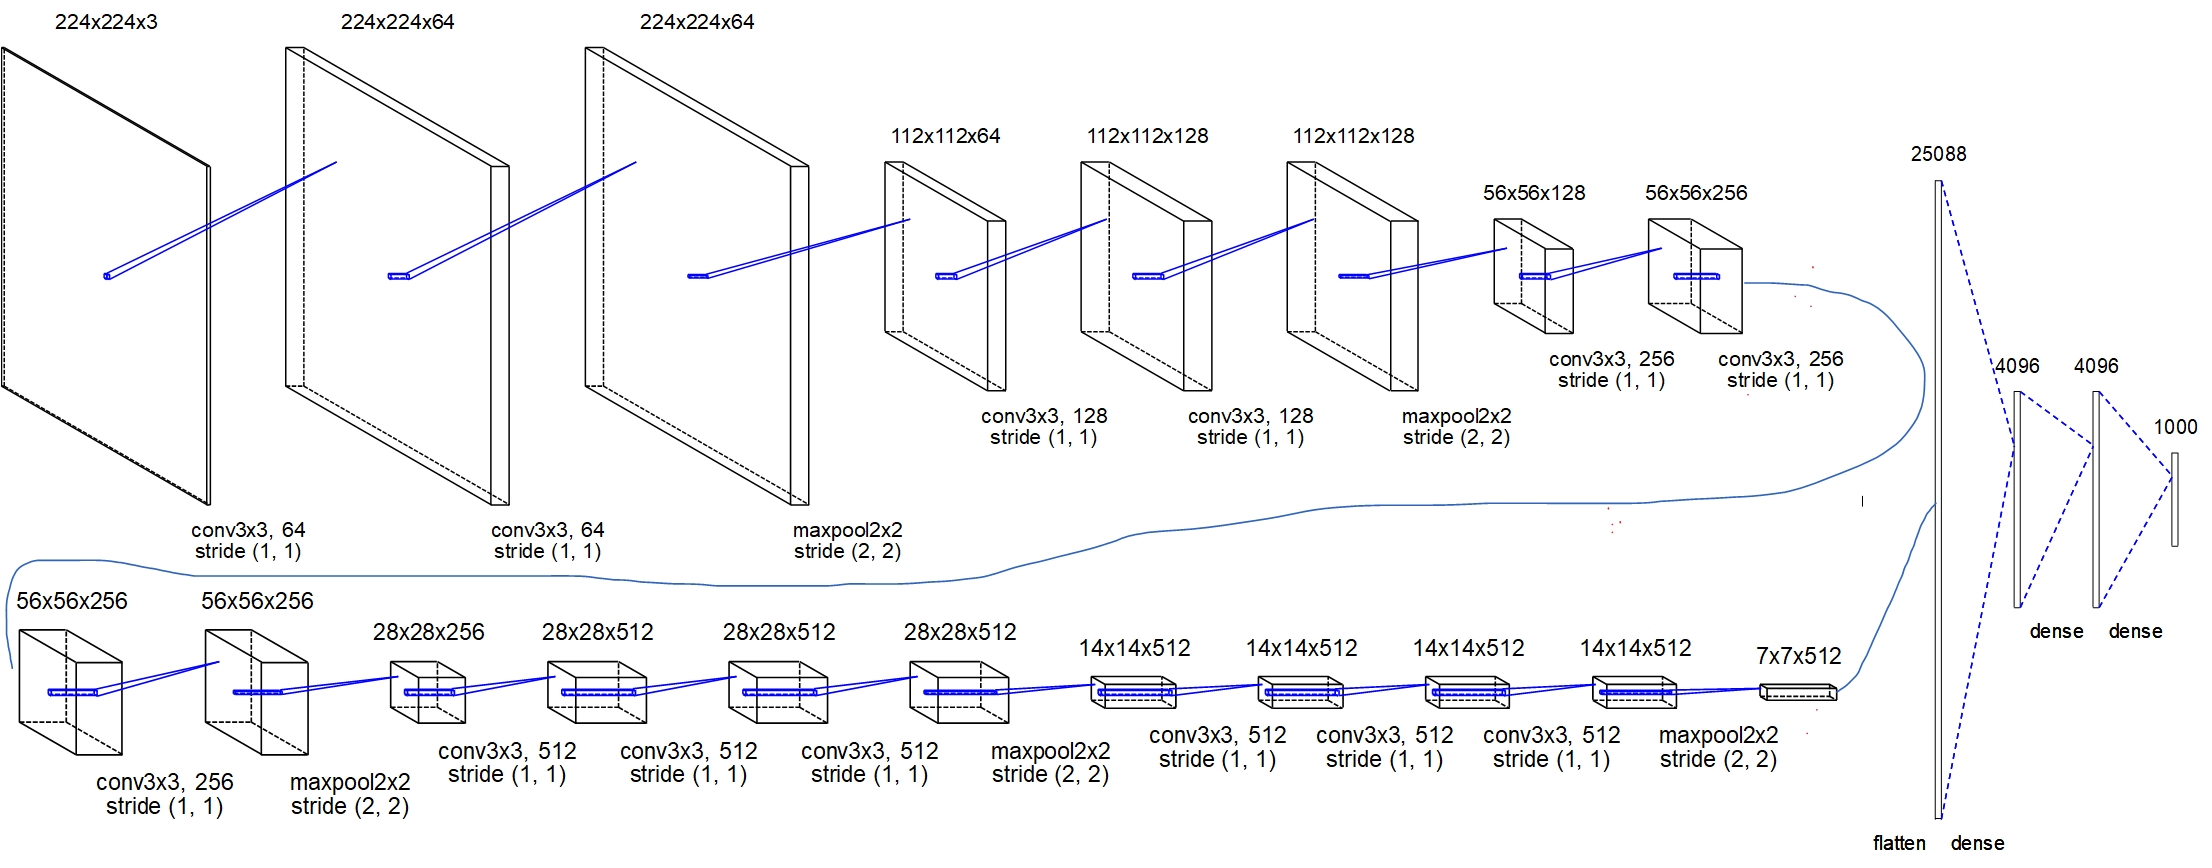
\includegraphics[scale=0.3]{14.jpg}
      \caption{VGG-16的卷积神经网络模型}
    \end{figure}
  
    VGG16共包含13个卷积层、3个全连接层和5个池化层。VGG-16的突出特点是简单,其卷积层采用相同的卷积核参数,池化层采用相同的池化和参数。模型是由若干卷积层和池化层堆叠的方式构成,比较容易形成较深的网络结构。
  \subsubsubsection{Fully-Convolutional Network}
   卷积层的每层数据是一个$h*w*d$的三维数组,其中$h$和$w$是空间维度,$d$是特征或通道维数。第一层是像素尺寸为$h*w$、颜色通道数为$d$的图像。高层中的位置和图像中它们连通的位置相对应,被称为接收域。

   卷积网是以平移不变性作为基础的。其基本组成部分(卷积、池化和激活函数)作用在局部输入域,只依赖相对空间坐标。在特定层记$X_{ij}$为在坐标$(i,j)$的数据向量,在接下来的层中有$Y_{ij}$,即\begin{gather}
     y_{ij}=f_{ks}(\{ x_{s_i+\delta_i,s_j+\delta_j} \}_{0\leq\delta_i,\delta_j\leq k})
   \end{gather}
  其中$k$为卷积核尺寸,$s$是步长或下采样因子,$f_{ks}$决定了层的类型:一个卷积的矩阵乘或者平均池化,用于最大池化的最大空间值或者是一个元素级的非线性激活函数,或者其他类型的网络层。
  
  上述过程的函数形式为\begin{gather}
    f_{ks}\circ g_{k's'}=(f\circ g)_{k'+(k-1)s',ss'}
  \end{gather}
  一个普通的深度神经网络计算一个普通的非线性函数,一个网络只有这种形式的层计算非线性滤波,我们称之为深度滤波或者全卷积网络\cite{7478072}。一个全卷积网络可以计算任意尺寸的输入并产生相应的输出。\begin{figure}[H]
    \setlength{\abovecaptionskip}{0.2cm}
    \setlength{\belowcaptionskip}{-0.cm}
      \centering%
      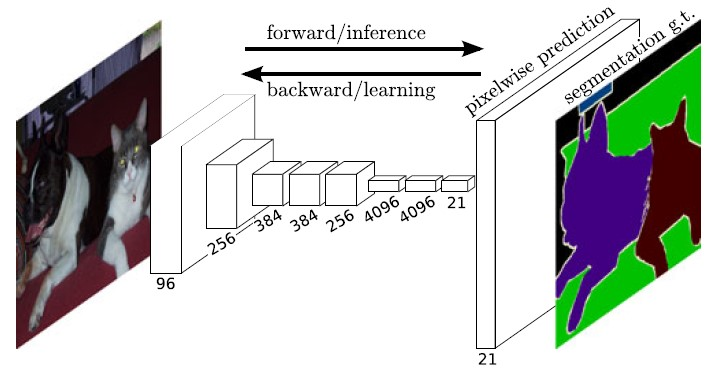
\includegraphics[scale=0.8]{15.jpg}
      \caption{全卷积网络的结构示意图}
    \end{figure}

  这里我们使用全卷积神经网络进行图像分割,即我们将图像分割问题转换为二分类问题,0表示背景,1表示花朵区域。\begin{figure}[H]
    \setlength{\abovecaptionskip}{0.2cm}
    \setlength{\belowcaptionskip}{-0.cm}
      \centering%
      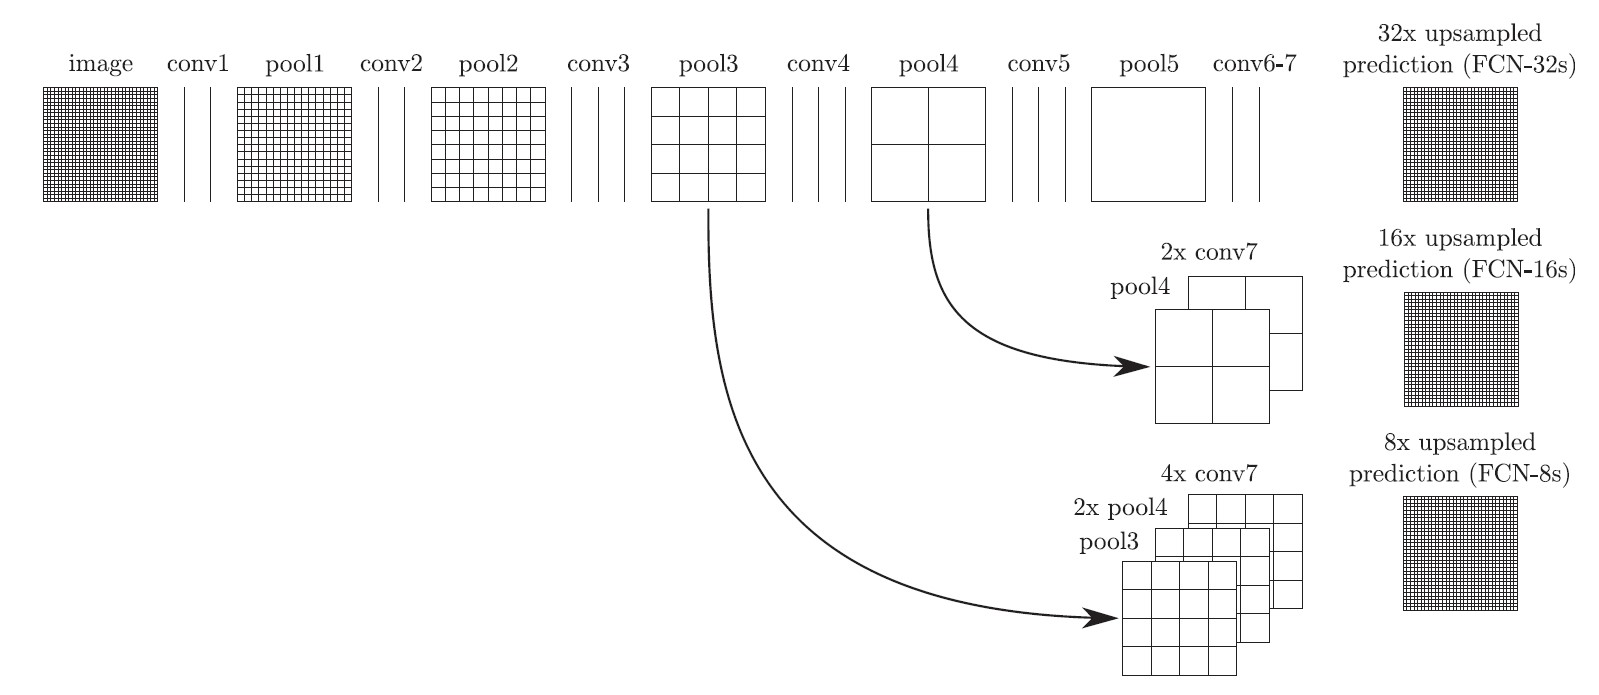
\includegraphics[scale=0.42]{18.jpg}
      \caption{全卷积网络用于分割问题的网络结构图}
    \end{figure}

  图2-13所示是全卷积神经网络用于分割问题的网络结构图。这里需要将粗糙的、高层信息与精炼的、低层信息结合起来。池化和预测层在图2-13表示为揭示表示空间密集程度的网格,同时中间层用两条竖线表示。FCN32s是在单步中上采样步长为32的预测值回到像素;FCN16s是以16为步长,结合pool4层和最终层的信息,可以得到更精炼的细节信息,同时包含高层次的语义信息;FCN8s更进一步,将pool3层的信息,以步长为8,与之前信息结合用于提高精度。本次课程设计中我们采用的正是FCN8s。
  \subsubsection{Snapshot Ensembles}
  Snapshot Ensembling\cite{DBLP:journals/corr/HuangLPLHW17}在一次训练过程中产生一组正确且具有多样性的分类模型,并进行集成。Snapshot Ensembling的核心是在收敛到最终解之前寻找到多个局部最优。我们利用这些得到的局部最优解模型,在测试时平均它们的预测输出。

  集成学习在每一个基模型有低测试误差且它们的错分类样本没有重叠。在大多数优化路径中,一个神经网络的权重赋值往往不等同于低测试误差。实际上,常常可以看到在只有在学习率下降的时候验证误差才显著下降,尤其是在几百个训练回合之后。我们的方法受到训练更好的回合和更早衰减学习率的启发,它们被证实可以减少对最终测试误差的影响。

  循环余弦退火(Cyclic Cosine Annealing):为了收敛到多个局部最优,我们采用循环余弦退火机制。我们以一个很快的速度降低学习率,鼓励模型在50个回合之内收敛到它的第一个局部最优。随后,优化过程继续以一个较大的学习率开始,即让模型从当前局部最优中跳出。我们重复几次上诉操作可以得到多个局部最优解。正式地说,对于学习率$\alpha$有\begin{gather}
    \alpha(t)=f(\text{mod}(t-1,[T/M]))
  \end{gather}
  这里$t$是迭代次数,$T$训练迭代总次数,$f$是一个单调下降的函数。换句话说,我们将训练过程分为$M$循环,每一个循环以一个较大的学习率开始,逐渐退火到一个较小的学习率。这个较大的$\alpha=f(0)$必须能够提供足够的能量让模型从当前局部最优中跳出,同时较小的学习率$\alpha=f([T/M])$让模型收敛到一个较好的局部最优解。在这里,我们设定$f$是移位余弦函数,即\begin{gather}
     \alpha(t)=\dfrac{\alpha_0}{2}\left( \cos\left( \dfrac{\pi\text{mod}(t-1,[T/M])}{[T/M]} \right)+1 \right)
  \end{gather}
  这里$\alpha_0$是初始学习率。直觉上讲,这个函数在一个训练循环中从初始学习率退火到接近0。我们在每一次迭代中就更新学习率,这样可以提高在少回合情况下的快速收敛。\begin{figure}[H]
    \setlength{\abovecaptionskip}{0.2cm}
    \setlength{\belowcaptionskip}{-0.2cm}
    \centering%
    \subcaptionbox{Snapshot ensembles的收敛路径} %标题的长度,超过则会换行,如下一个小图。
      {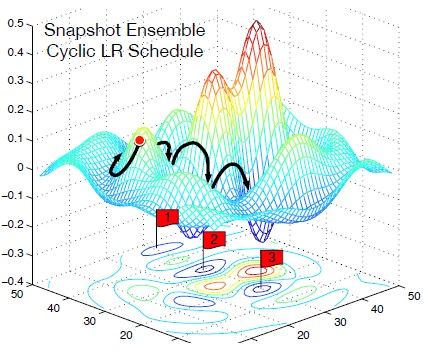
\includegraphics[height=5cm]{16.jpg}}%
    \hspace{2em}%
    \subcaptionbox{Snapshot ensembles的学习率曲线}
        {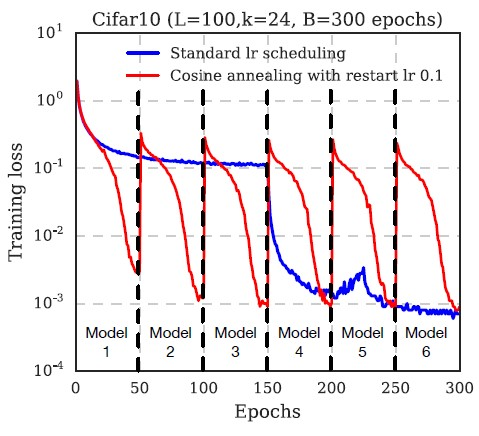
\includegraphics[height=5cm]{17.jpg}}
  
    \caption{Snapshot ensembles}
    \end{figure}

  Snapshot Ensembling:在每一次训练循环的末尾,很显然这时模型已经找到了一个局部最优解。这样,在提升学习率之前,我们将这时的模型保存下来,成为Snapshot。在$M$个循环之后,我们得到了$M$个模型,即$f_1,\dots,f_M$。更重要的是等到这一系列模型的时间与之前用标准训练方法得到一个模型的时间一样。

  在测试环节中,集成输出是将最后$m$个模型的输出进行平均。令$x$是一个测试样本,$h_i(x)$是第$i$个模型的softmax输出。输出的结果为\begin{gather}
    h_{\text{Ensemble}}=\dfrac{1}{m}\sum\limits^{m-1}_{i=0}h_{M-i}(x)
  \end{gather}

  第二章主要介绍了我们这次课程设计所使用的主要原理,下面将介绍本次课程设计的实验系统设计方案。
  \section{实验系统设计}
  \subsection{总体算法流程图}
  在本次课程设计中,我们将花卉识别分为3个模块:分割模块、特征提取模块和分类模块,图3-1所示是此次所采用的对应模块所采用的算法和大致流程。\begin{figure}[H]
    \setlength{\abovecaptionskip}{0.2cm}
    \setlength{\belowcaptionskip}{-0.cm}
      \centering%
      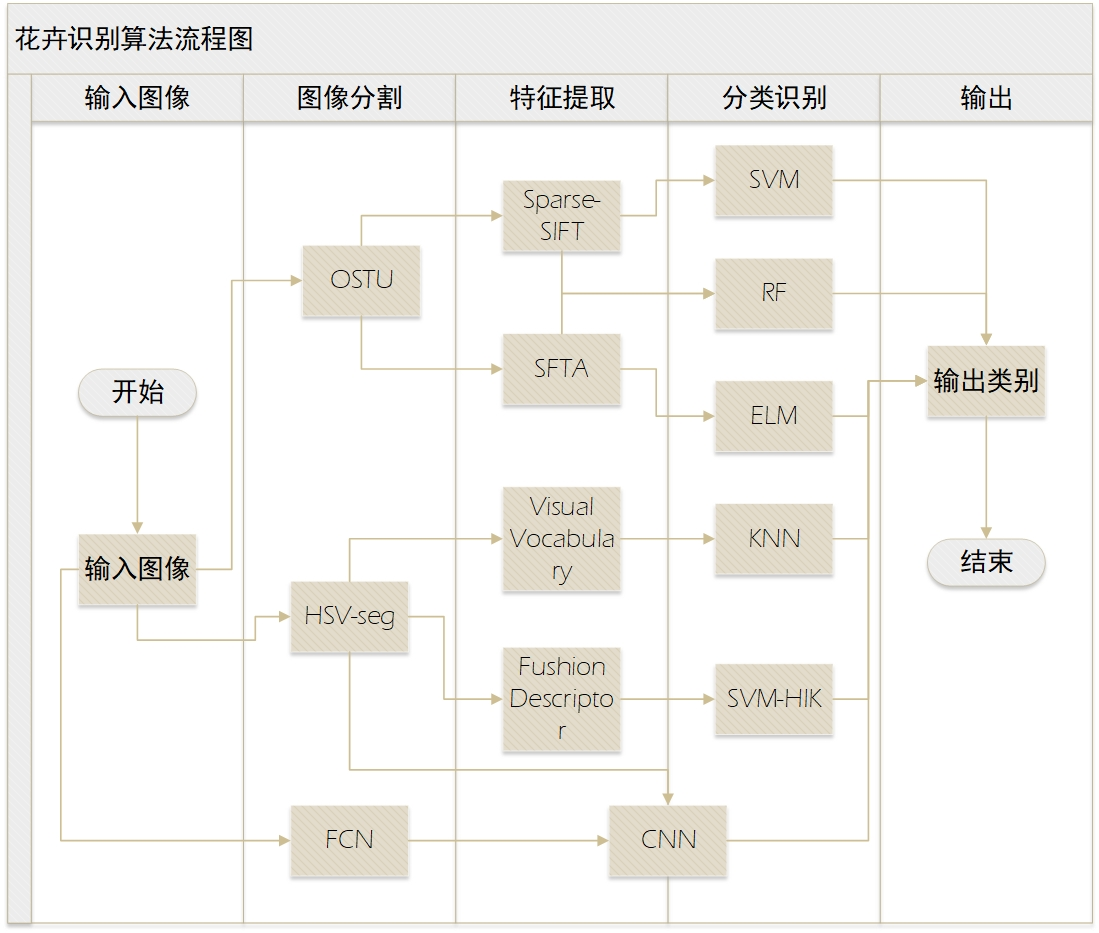
\includegraphics[scale=0.6]{19.jpg}
      \caption{总体算法流程图}
    \end{figure}
  
  如图3-1所示,本次课程设计采用了多种花卉分类方法,意图在于比较各种方法的优缺点和差异,即\begin{itemize}
  \item 方案一:基于视觉词汇的花卉识别方法\cite{1640927}(HSV-seq+Visual Vocabulary+KNN);
  \item 方案二:基于融合特征描述子的花卉识别方法\cite{8090865}(HSV-seq+Fushion Descriptor+SVM-HIK);
  \item 方案三:基于Sparse-SIFT的花卉识别方法\cite{6968612}(OSTU+Sparse-SIFT+SVM/RF/ELM);
  \item 方案四:基于SFTA的花卉识别方法\cite{6968612}(OSTU+SFTA+SVM/RF/ELM);
  \item 方案五:基于卷积神经网络的花卉识别方法\cite{1640927};
  \item 方案六:基于迁移学习的卷积神经网络的花卉识别方法\cite{8600536};
  \item 方案七:基于全卷积神经网络和迁移学习的花卉识别方法\cite{8435127}(FCN+CNN)。
  \end{itemize}

  下面几个小节将逐一介绍每一种方案的各个模块的具体细节。
  \subsection{方案一:基于视觉词汇的花卉识别方法}
  \subsubsection{算法流程}
  基于视觉词汇的花卉识别方法是对一幅花卉图像分别提取其颜色、形状和纹理特征,其中颜色特征是使用HSV颜色空间;形状特征使用SIFT算子;纹理特征使用LBP算子。在应用过程中,对于HSV颜色空间和LBP算子运算过后的图像,我们不采用逐个像素进行聚类,而对每行和每列分别求一个均值和协方差矩阵,将均值和铺平后的协方差矩阵拼接成一个向量,作为这一行或列的特征表示。如图3-2所示是方案一的算法流程图:\begin{figure}[H]
    \setlength{\abovecaptionskip}{0.2cm}
    \setlength{\belowcaptionskip}{-0.cm}
      \centering%
      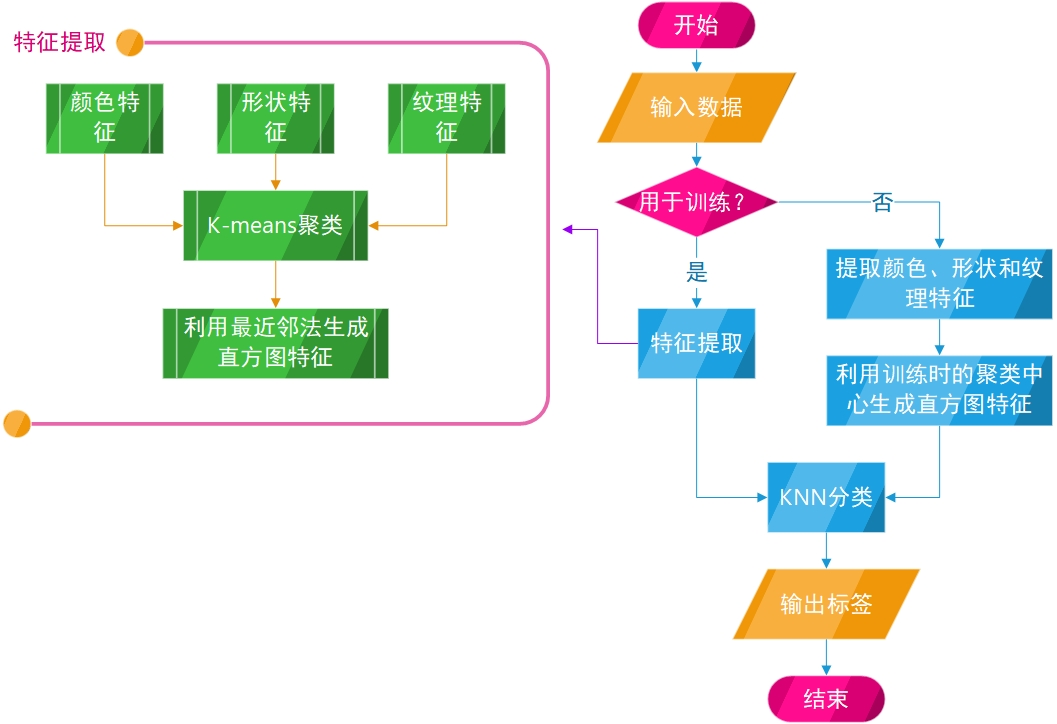
\includegraphics[scale=0.62]{22.jpg}
      \caption{基于视觉词汇的花卉识别算法流程图}
    \end{figure}
  \subsubsection{程序模块说明}
  关于方案一的模块说明如表3-1所示。
  \begin{spacing}{1.25}
  \begin{longtable}[c]{p{0.28\textwidth}p{0.66\textwidth}}
    \caption{方案一的程序模块说明}\label{tab:performance}\\
    \toprule[1.5pt]
     程序文件名或函数名 & 模块说明 \\\midrule[1pt]
    \endfirsthead
    \multicolumn{2}{c}{续表~\thetable\hskip1em 方案一的程序模块说明}\\
    \toprule[1.5pt]
    程序文件名或函数名 & 模块说明 \\\midrule[1pt]
    \endhead
    \hline
    \multicolumn{2}{r}{续下页}
    \endfoot
    \endlastfoot
    main.py&该文件是方案一的主函数模块,包含该方案算法流程的全过程:读取文件、特征提取、分类识别输出和测试正确率,得到最终结果。\\
    \midrule[1pt]
    randomSample&在花卉数据集中每一个类别文件夹中,随机生成索引选择出指定个数的样本作为训练样本,其余作为测试样本\\
    load&加载数据,其中参数mode="color"表示提取颜色特征;mode="shape"表示提取形状特征;mode="texture"表示提取纹理特征,最终返回样本数据和每一幅图像提取的特征个数组成的数组。\\
    \midrule[1pt]
    chi2\_distance&计算$\chi^2$统计量距离\\
    plot\_embedding&用于t-SNE的可视化函数\\
    segmentation&分割图片,利用基于HSV的分割算法分割花卉图像,并返回分割后的图像\\
    \midrule[1pt]
    xkNN&基于$\chi^2$统计量距离的单一特征的KNN分类器\\
    bxNN&基于$\chi^2$统计量距离的联合特征的KNN分类器\\
    ekNN&基于欧式距离的kNN分类器\\
    featureCOV&用于测试样本提取颜色特征\\
    featureSIFT&用于测试样本提取形状特征\\
    featureLBP&用于测试样本提取纹理特征\\
    \bottomrule[1.5pt]
    \end{longtable}
  \end{spacing}
  程序对应在文件夹test中。
  \subsection{方案二:基于融合特征描述子的花卉识别方法}
  \subsubsection{算法流程}
  基于融合特征描述子的花卉识别方法是通过提取颜色和纹理特征,同时也考虑形状特征的作用,利用PHOW特征生成框架生成对应的特征;提取颜色特征时,主要使用denseSIFT算子;提取纹理特征时,主要使用在灰度图上的denseSIFT算子;提取形状特征时,则使用基于edgeSIFT的方法。在提取特征之后,采用LLC编码方式,主要考虑特征样本的局部分布约束,保持局部距离。图3-3所示是该方案的算法流程图。\begin{figure}[H]
    \setlength{\abovecaptionskip}{0.2cm}
    \setlength{\belowcaptionskip}{-0.cm}
      \centering%
      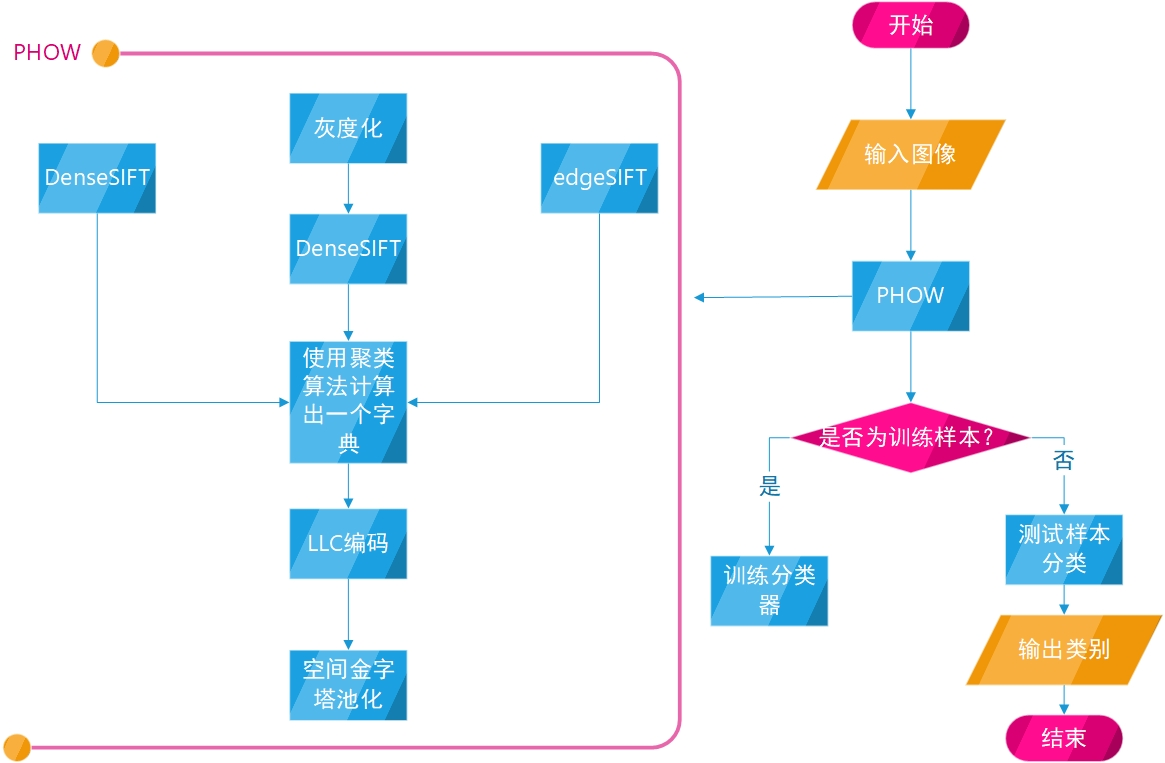
\includegraphics[scale=0.55]{23.jpg}
      \caption{基于融合特征描述子的花卉识别算法流程图}
    \end{figure}
  \subsubsection{程序模块说明}
  关于方案二的模块说明如表3-2所示。
  \begin{spacing}{1.25}
    \begin{longtable}[c]{p{0.28\textwidth}p{0.66\textwidth}}
      \caption{方案二的程序模块说明}\label{tab:performance}\\
      \toprule[1.5pt]
       程序文件名或函数名 & 模块说明 \\\midrule[1pt]
      \endfirsthead
      \multicolumn{2}{c}{续表~\thetable\hskip1em 方案二的程序模块说明}\\
      \toprule[1.5pt]
      程序文件名或函数名 & 模块说明 \\\midrule[1pt]
      \endhead
      \hline
      \multicolumn{2}{r}{续下页}
      \endfoot
      \endlastfoot
      main.py&该文件是方案二的主函数模块,包含该方案算法流程的全过程:读取文件、特征提取、生成特征数据文件、(直接读取生成特征数据文件)、分割训练集和测世界、分类识别输出和测试正确率,得到最终结果。\\
      \midrule[1pt]
      dSIFT.py&该文件定义了方案二所采用的denseSIFT特征提取算子,其余文件可直接调用\\
      \midrule[1pt]
      matrixPow&矩阵乘方函数,即计算$X^{\gamma}$\\
      splitImage、splitGEImage&按空间金字塔要求将图像4等分\\
      segmentation&图像分割函数,使用HSV-sep分割算法\\
      getCodebook&通过聚类获得编码字典\\
      LLCoding&计算LLC编码\\
      saveCodebook&保存编码字典\\
      extractHSVCodebook、extractGCodebook、extractECodebook&提取HSV、Gray和edge-SIFT的编码字典和特征编码\\
      PHOW\_HSV、PHOW\_G、PHOW\_E&提取HSV、Gray和edge-SIFT的PHOW特征\\
      saveHSVcode、saveGcode、saveECode&保存HSV、gray和edge-SIFT的特征编码\\
      \midrule[1pt]
      msvm.py&定义HIK核函数,并用于SVM分类器\\
      \bottomrule[1.5pt]
      \end{longtable}
    \end{spacing}
    程序对应在文件夹fsvm中。
  \subsection{方案三:基于Sparse-SIFT的花卉识别方法}
  \subsubsection{算法流程}
  基于Sparse-SIFT的花卉识别方法是提取图像的SIFT特征,再利用K-SVD将其进行稀疏编码。在本次课程设计的过程中,我们采用3.3节中已经有的denseSIFT特征算子提取图像的特征,再进行K-SVD稀疏编码。图3-4所示为方案三的算法流程图。\begin{figure}[H]
    \setlength{\abovecaptionskip}{0.2cm}
    \setlength{\belowcaptionskip}{-0.cm}
      \centering%
      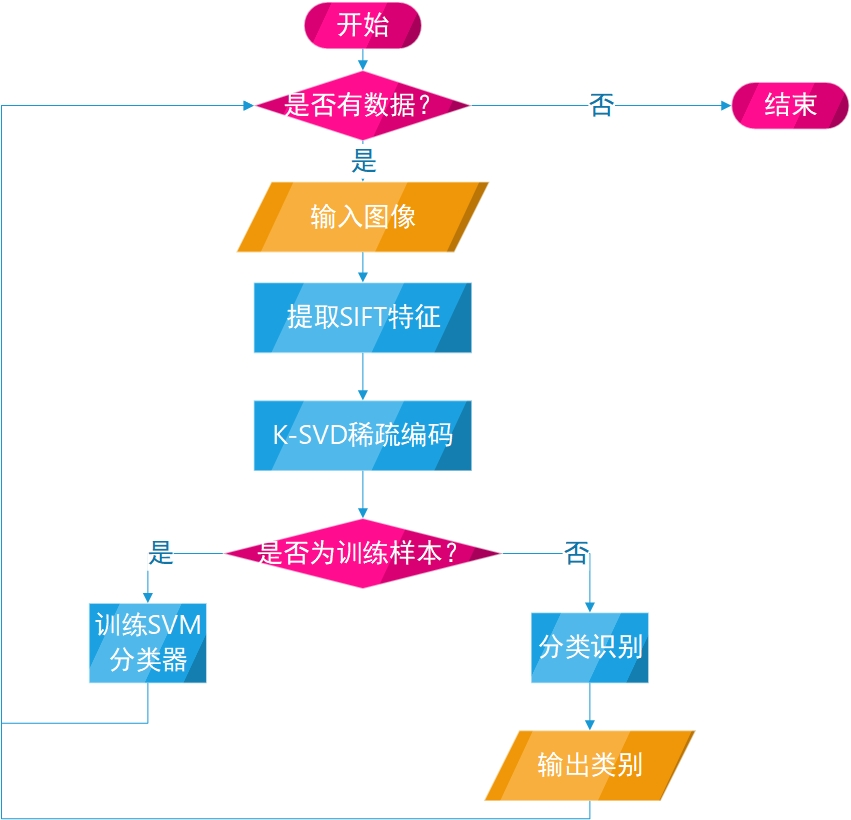
\includegraphics[scale=0.55]{24.jpg}
      \caption{基于Sparse-SIFT的花卉识别算法流程图}
    \end{figure}
  \subsubsection{程序模块说明}
  关于方案三的模块说明如表3-3所示。
  \begin{spacing}{1.25}
    \begin{longtable}[c]{p{0.28\textwidth}p{0.66\textwidth}}
      \caption{方案三的程序模块说明}\label{tab:performance}\\
      \toprule[1.5pt]
       程序文件名或函数名 & 模块说明 \\\midrule[1pt]
      \endfirsthead
      \multicolumn{2}{c}{续表~\thetable\hskip1em 方案三的程序模块说明}\\
      \toprule[1.5pt]
      程序文件名或函数名 & 模块说明 \\\midrule[1pt]
      \endhead
      \hline
      \multicolumn{2}{r}{续下页}
      \endfoot
      \endlastfoot
      main.py&该文件是方案三的主函数模块,包含该方案算法流程的全过程:读取文件、特征提取、生成特征数据文件、(直接读取生成特征数据文件)、分割训练集和测世界、分类识别输出和测试正确率,得到最终结果。\\
      \midrule[1pt]
      plot\_embedding&t-SNE的可视化绘图函数\\
      loadSIFT&用于SIFT特征提取的数据加载函数,读入图片并将其转化为灰度图用于后续SIFT特征提取\\
      \midrule[1pt]
      sSIFT.py&该文件定义了方案三所采用的denseSIFT特征提取算子,其余文件可直接调用。先用滑动窗口将图像划分为多个重叠的网格,再在每一个小窗口上提取SIFT特征,再进行整合计算得到最终结果\\
      \midrule[1pt]
      ksvd.py&该文件定义了方案三采用的稀疏编码方式K-SVD\\
      \midrule[1pt]
      segment&基于OTSU方法的图像分割函数,这里为了提高运算速度我们使用了opencv自带的OTSU阈值分割方法\\
      SIFT&稀疏编码的SIFT特征提取函数,先提取SIFT特征,再将其用K-SVD稀疏编码方式得到SIFT特征的稀疏编码并返回稀疏编码特征\\
      \bottomrule[1.5pt]
      \end{longtable}
    \end{spacing}
    程序对应在文件夹fSVMoRF中。
  \subsection{方案四:基于SFTA的花卉识别方法}
  \subsubsection{算法流程}
  基于SFTA的花卉识别方法是一种比较新颖的针对花卉的特征提取方法,主要针对纹理特征。主要分为两个部分:1)把输入的灰度图像分解成一系列二值图像,这里采用两阈值二值化分解进行二值化;2)对于上述得到的二值化图像,我们计算区域的边界的分形维度,另外在计算区域的平均灰度值和面积。对于多等级OTSU算法,寻找到阈值能够使输入的图像的类内方差最小化;然后,以递归的方式不断对每一幅输入图像区域应用OTSU算法直到指定个数的阈值;计算分形维度时,可以通过Box Counting算法计算分形维度的近似值,和平均灰度值、区域面积一起拼接成最终的SFTA特征。\begin{figure}[H]
    \setlength{\abovecaptionskip}{0.2cm}
    \setlength{\belowcaptionskip}{-0.cm}
      \centering%
      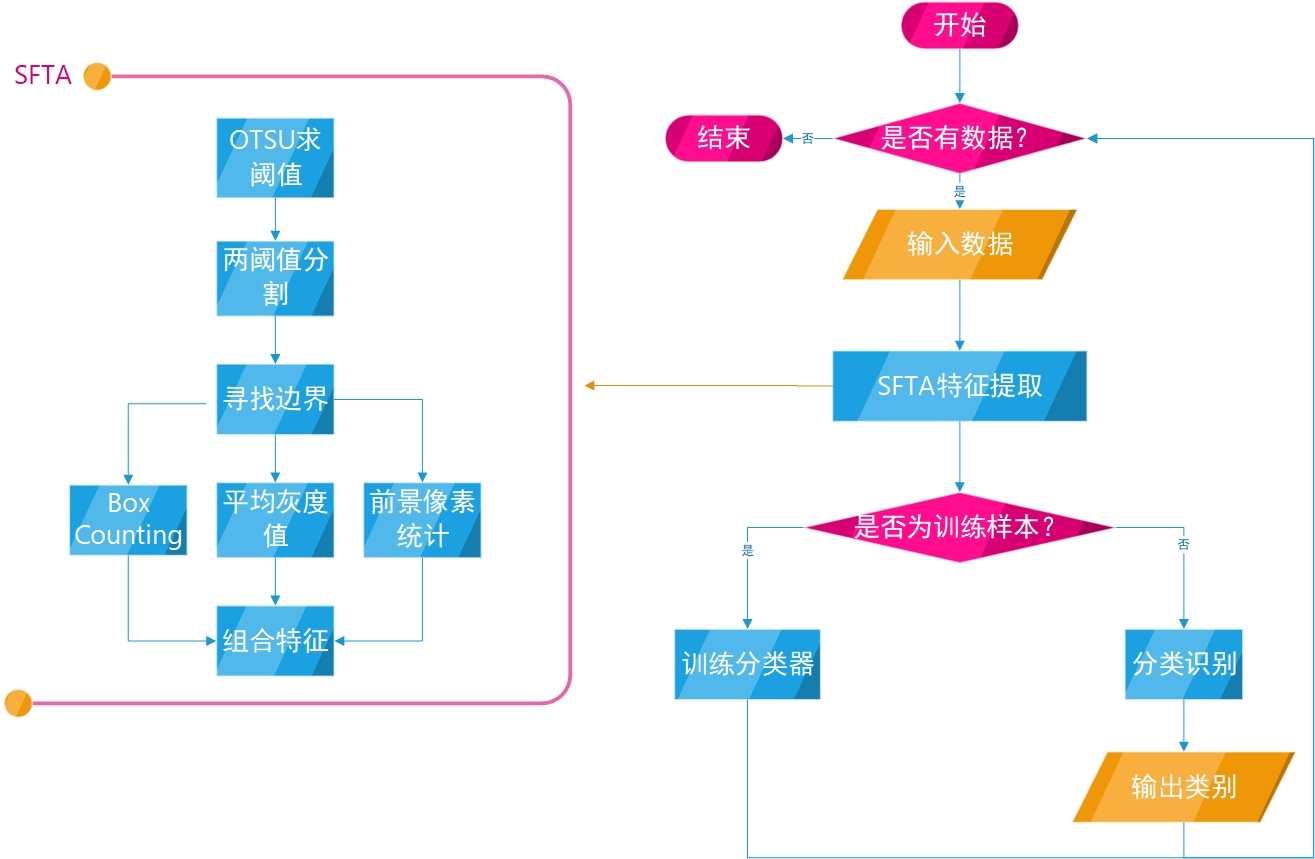
\includegraphics[scale=0.5]{25.jpg}
      \caption{基于SFTA的花卉识别算法流程图}
    \end{figure}
  \subsubsection{程序模块说明}
  关于方案四的模块说明如表3-4所示。
  \begin{spacing}{1.25}
    \begin{longtable}[c]{p{0.28\textwidth}p{0.66\textwidth}}
      \caption{方案四的程序模块说明}\label{tab:performance}\\
      \toprule[1.5pt]
       程序文件名或函数名 & 模块说明 \\\midrule[1pt]
      \endfirsthead
      \multicolumn{2}{c}{续表~\thetable\hskip1em 方案三的程序模块说明}\\
      \toprule[1.5pt]
      程序文件名或函数名 & 模块说明 \\\midrule[1pt]
      \endhead
      \hline
      \multicolumn{2}{r}{续下页}
      \endfoot
      \endlastfoot
      main.py&该文件是方案四的主函数模块,包含该方案算法流程的全过程:读取文件、特征提取、生成特征数据文件、(直接读取生成特征数据文件)、分割训练集和测世界、分类识别输出和测试正确率,得到最终结果。\\
      \midrule[1pt]
      plot\_embedding&t-SNE的可视化绘图函数\\
      load&用于SFTA特征提取的数据加载函数,加载文件图片并缩放到$330\times250$,并提取SFTA特征\\
      \midrule[1pt]
      sfta.py&定义提取sfta特征的一系列函数\\
      \midrule[1pt]
      elm.py&极限学习机模块,定义极限学习机模型,并读取已经得到的特征进行分类\\
      \midrule[1pt]
      pseudoInv.py&用于极限学习机训练的伪逆求解模块,通过迭代方式求解伪逆\\
      \bottomrule[1.5pt]
      \end{longtable}
    \end{spacing}
    程序对应在文件夹fSVMoRF中。
  \subsection{方案五:基于卷积神经网络的花卉识别方法}
  基于卷积神经网络的花卉识别方法是利用卷积神经网络的方法,通过神经网络自动提取特征和完成分类。实践证明,深度卷积神经网络的分类性能会高于人工提取的特征得到的分类性能。在训练网络过程中,我们对学习率的选择进行了改变,采用了snapshot ensembles方式,可以训练一次得到多个模型进行集成得到结果,后面两种方案也同样采取这种方式。图3-5所示是本方案所使用的卷积神经网络结构图。\begin{figure}[H]
    \setlength{\abovecaptionskip}{0.2cm}
    \setlength{\belowcaptionskip}{-0.cm}
      \centering%
      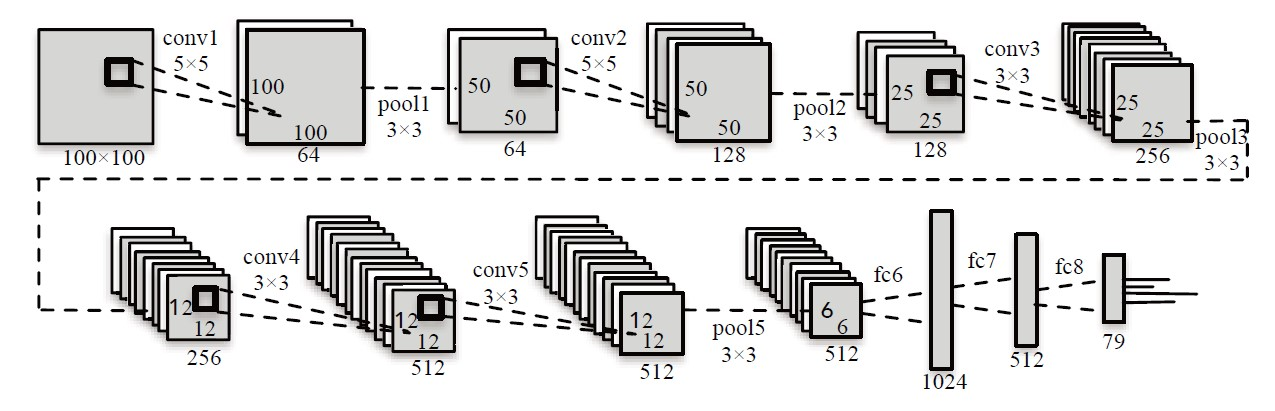
\includegraphics[scale=0.5]{26.jpg}
      \caption{方案五的卷积神经网络结构图}
    \end{figure}
  
  图像通过一组卷积层。第一卷积层有64个卷积核,大小为$5\times5\times3$,输入图像的大小为$100\times100\times3$。第二、三层卷积层网络分别包含128、256个卷积核,其大小分别为$5\times5\times64$和$3\times3\times128$连接到前一卷积层的输出,包括归一化和池化。第四卷积层把池化后的第三卷积层的输出作为输入,带有512个卷积核,其大小为$3\times3\times256$,第五卷积层包含512个卷积核,其大小为$3\times3\times512$。卷积核的步长为1个像素,对于$5\times5$的卷积核补全宽度为2个像素,对于$3\times3$的卷积核补全宽度为1个像素。在一系列卷积层之后接入到全连接层中,前两层分别包含1024和512个神经元,最后一层的神经元个数与对应分类问题的类别一致。空间池化由4个最大池化层完成,池化核大小为$3\times3$,步长为2个像素。在所有卷积层和全连接层后接入ReLU非线性激活函数。
  \subsection{方案六:基于迁移学习的卷积神经网络的花卉识别方法}
  迁移学习是当前机器学习中一个十分重要的分支。迁移学习的最初意图受到人类思维的启发,人们在面对相似但从未见过的问题时可以根据以往的经验对新的问题作出判断,这过程往往具有很高的确信度。ImageNet是一个庞大的图像数据库,其中包含很多很多种类的图像。显然,花卉识别与ImageNet中的图像识别是相似的任务,即可以用ImageNet训练好的神经网络模型用来对花卉进行识别。由于花卉识别与ImageNet的识别任务事实上有一定的差别,可以对已经训练好的神经网络模型进行微调,这里我们将VGG16的神经网络模型的最后一个全连接层替换成自定义的全连接层,输出神经元个数与我们所需分类的类别数相同。我们固定除自定义层参数之外的其他参数,用ImageNet已经训练好的模型参数对应代入,再对最后一层进行训练从而完成对神经网络的微调,从而完成训练过程,实现花卉识别。\begin{figure}[H]
    \setlength{\abovecaptionskip}{0.2cm}
    \setlength{\belowcaptionskip}{-0.cm}
      \centering%
      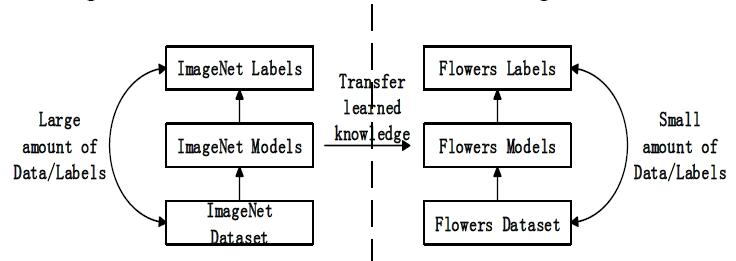
\includegraphics[scale=0.6]{29.jpg}
      \caption{迁移学习示意图}
    \end{figure}\begin{figure}[H]
      \setlength{\abovecaptionskip}{0.2cm}
      \setlength{\belowcaptionskip}{-0.cm}
        \centering%
        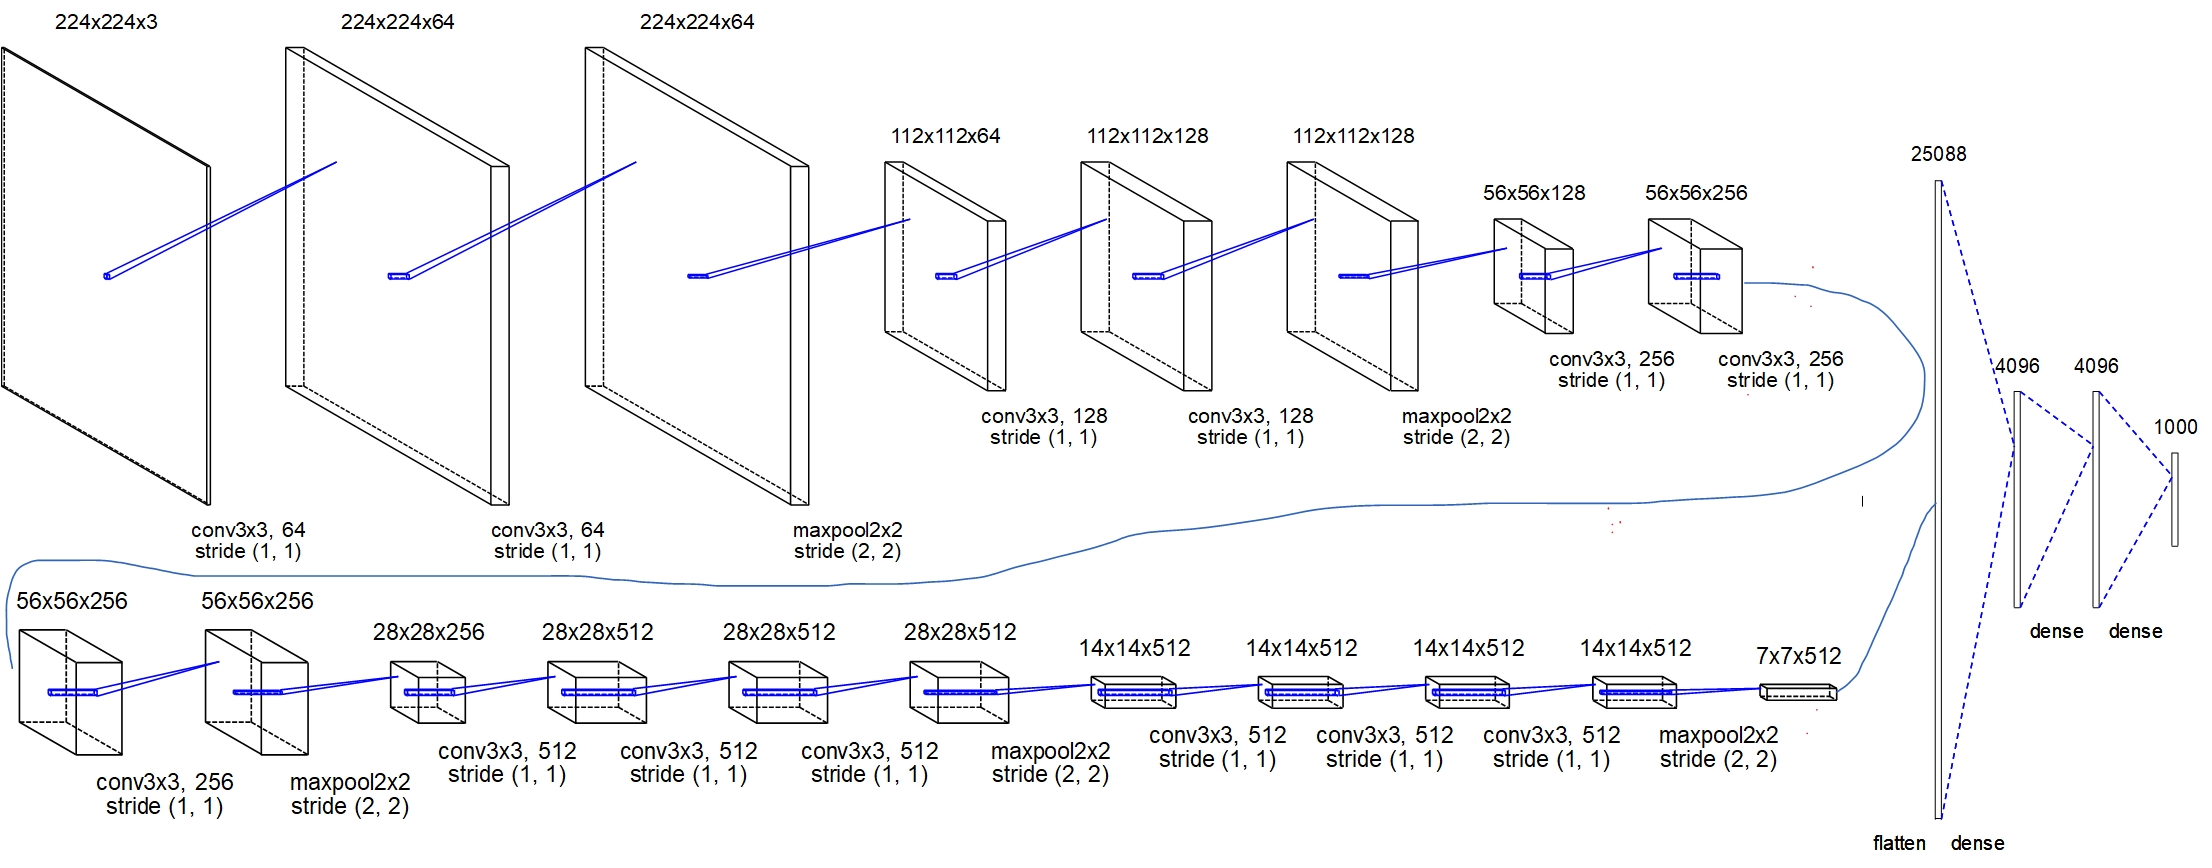
\includegraphics[scale=0.3]{14.jpg}
        \caption{VGG16神经网络结构图}
    \end{figure}
  \subsection{方案七:基于全卷积神经网络和迁移学习的花卉识别方法}
  全卷积神经网络是用于图像分割的有力工具。我们同样借用迁移学习的思想,对全连接神经网络使用预训练好的VGG16模型确定全卷积神经网络的卷积层参数,再通过训练后面的解卷积层得到最终的全卷积神经网络模型。后面对于用FCN进行图像分割的图片再用方案六所述的基于迁移学习的卷积神经网络进行训练和得到分类结果。图3-9所示是该方案的整体流程图,图3-10所示是使用预训练模型参数的神经网络参数结构图。\begin{figure}[H]
    \setlength{\abovecaptionskip}{0.2cm}
    \setlength{\belowcaptionskip}{-0.cm}
      \centering%
      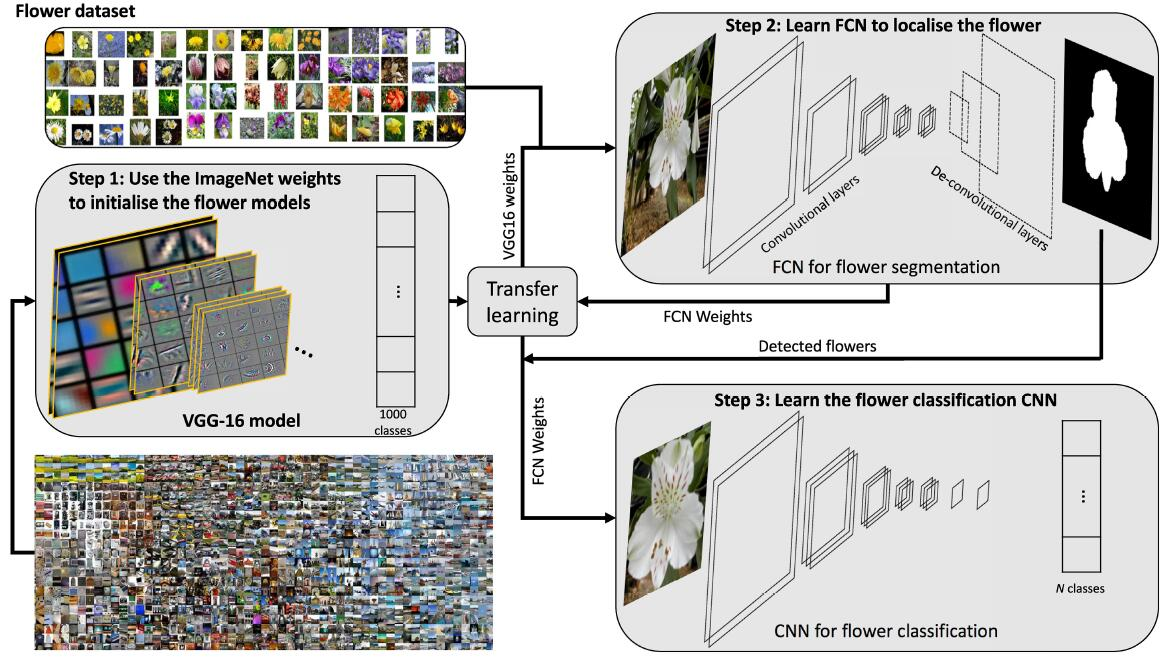
\includegraphics[scale=0.45]{27.jpg}
      \caption{花卉分割和识别框架}
    \end{figure}\begin{figure}[H]
      \setlength{\abovecaptionskip}{0.2cm}
      \setlength{\belowcaptionskip}{-0.cm}
        \centering%
        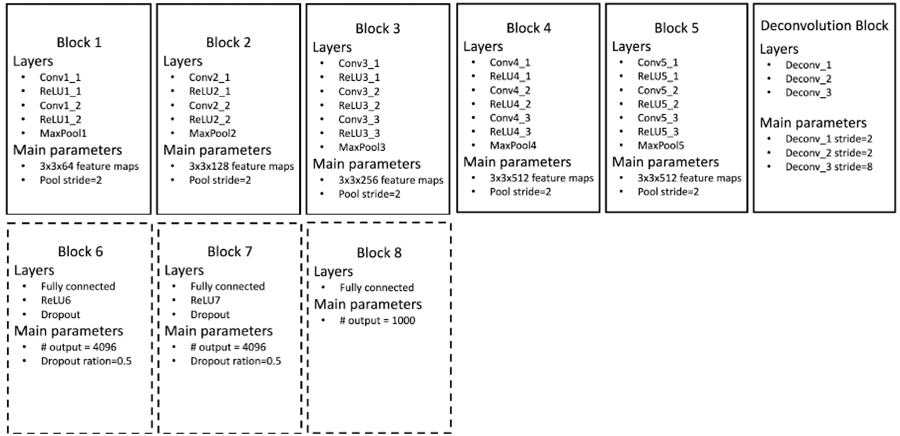
\includegraphics[scale=0.7]{28.jpg}
        \caption{神经网络参数和结构示意图}
    \end{figure}

  本章主要介绍了本次课程设计的实验系统方案设计,主要陈述所采用的几个方案的主要流程和一些程序模块说明。接下来我们将展示本次课程设计的实验结果并进行分析。
  % \begin{figure}[H]
  %   \begin{minipage}{0.48\textwidth}
  %     \centering
  %     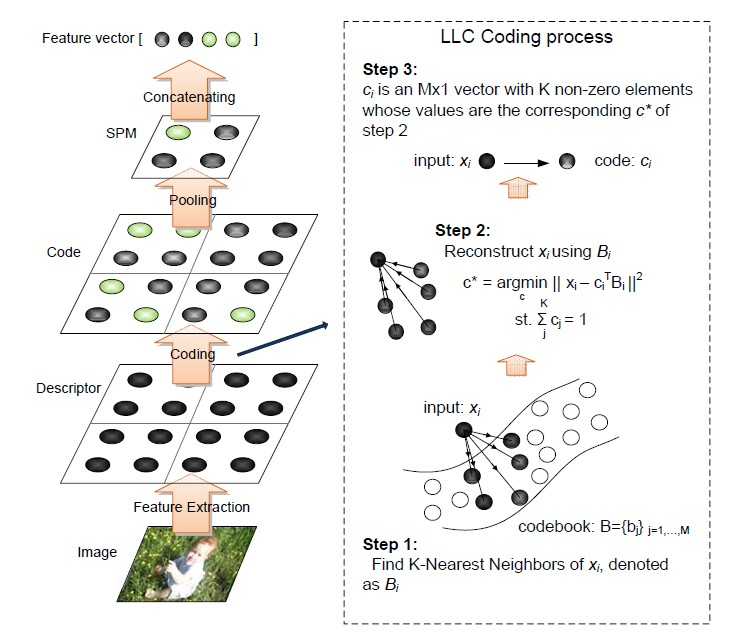
\includegraphics[height=5cm]{11.jpg}
  %     \caption{LLC编码过程}
  %     \label{fig:parallel1}
  %   \end{minipage}\hfill
  %   \begin{minipage}{0.48\textwidth}
  %     \centering
  %     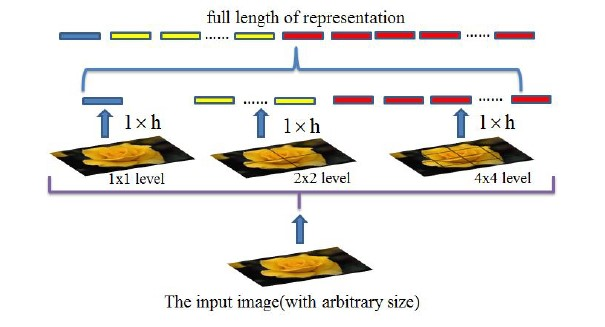
\includegraphics[height=5cm]{10.jpg}
  %     \caption{空间金字塔池化}
  %     \label{fig:parallel2}
  %   \end{minipage}
  %   \end{figure}
  % \begin{algorithm}[H] 
  %   \caption{Tangent Space Features-Based Transfer Learning} 
  %   \label{alg:Framwork} 
  %   \begin{algorithmic}[1] %这个1 表示从第一行开始显示行号,不写就不会显示行号
  %   \REQUIRE ~~\\ %算法的输入参数:Input
  %   $\theta$ \\
  %   \ENSURE ~~\\ %算法的输出:Output
  %   \STATE Initialize: $\{ (\Sigma,\mu) \}=\{ I,0 \}$
  %   \REPEAT
  %   \STATE Update $w_s=\left( \dfrac{1}{\theta}X^T_sX_s+\mu^{-1} \right)^{-1}\left( \dfrac{1}{\theta}X^T_sy_s+\mu^{-1}\Sigma \right)$
  %   \STATE Update $\Sigma=\dfrac{\sum^S_{s=1}(w_s-\mu)(w_s-\mu)^T}{\text{Tr}((w_s-\mu)(w_s-\mu)^T)}+\epsilon I$
  %   \STATE Update $\mu=\dfrac{1}{S}\sum^S_{s=1} w_s$
  %   \UNTIL converge.
  %   \RETURN $\{ (\Sigma,\mu) \}$; %算法的返回值
  %   \end{algorithmic}
  % \end{algorithm}
  \section{实验结果分析}
  \subsection{图片实验示例}
  \subsubsection{图片分割示例}
  这里我们展示图片的分割效果,用于测试的图片是我们实地真实拍摄的花卉图片,用于测试识别系统的泛化能力。
  \begin{figure}[H]
    \begin{minipage}[t]{0.24\textwidth}
    \centering
     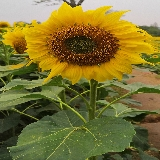
\includegraphics[scale=0.55]{te1.jpg}

     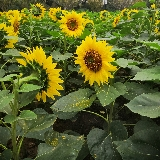
\includegraphics[scale=0.55]{te2.jpg}
 
     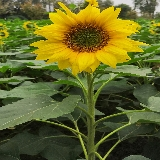
\includegraphics[scale=0.55]{te3.jpg}
     \subcaption{原始图像}
     \end{minipage}
     \begin{minipage}[t]{0.24\textwidth}
     \centering
     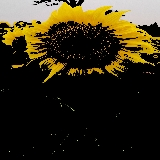
\includegraphics[scale=0.55]{seg11.jpg}
 
     
\includegraphics[scale=0.55]{seg21.jpg}
  
     
\includegraphics[scale=0.55]{seg31.jpg}
     \subcaption{基于HSV的分割}
     \end{minipage}
     \begin{minipage}[t]{0.24\textwidth}
      \centering
      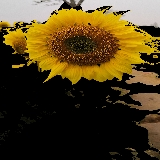
\includegraphics[scale=0.55]{seg12.jpg}
    
      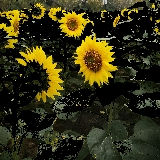
\includegraphics[scale=0.55]{seg22.jpg}
     
      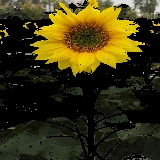
\includegraphics[scale=0.55]{seg32.jpg}
      \subcaption{基于OTSU的分割}
      \end{minipage}
      \begin{minipage}[t]{0.24\textwidth}
        \centering
        
\includegraphics[scale=0.55]{seg13.jpg}
    
        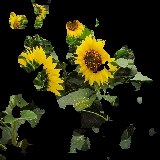
\includegraphics[scale=0.55]{seg23.jpg}
      
        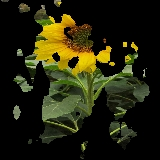
\includegraphics[scale=0.55]{seg33.jpg}
        \subcaption{基于FCN的分割}
        \end{minipage}
   \caption{图片分割示例}
   \end{figure}

   可以看出,上述花卉分割的方法是基于花朵的部分颜色比较鲜艳而背景比较暗淡,而我们是在白天拍摄的图片,天空背景等其余目标会极大影响分割的效果。

   从图4-1中看出,基于HSV颜色空间的图像分割算法和基于OTSU的颜色分割算法对于天空背景表现不佳,且基于OTSU的颜色分割算法对于复杂背景的表现较差,对于非花目标物体没有去除;而基于FCN的图像分割算法的结果较前两种算法有有一定的提升,但由于训练时的目标掩图存在噪声会影响最终的FCN模型的分割效果,但其对天空背景有一定的分割能力,但其分割效果缺乏解释性,对于一些分割出错的地方缺乏解释性。
   \subsubsection{图片识别示例}
   将4.1.1中的测试图片放入实验系统中,测试系统的分类能力,表4-1所示是每一种算法给出的分类结果,其中图片编号对应图4-2中所示的图片。
   \begin{figure}[H]
    \begin{minipage}[t]{0.24\textwidth}
    \centering
     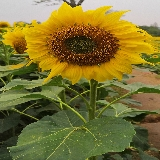
\includegraphics[scale=0.55]{te1.jpg}
     \subcaption{test1}
     \end{minipage}
     \begin{minipage}[t]{0.24\textwidth}
     \centering
     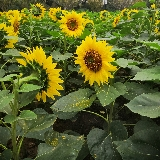
\includegraphics[scale=0.55]{te2.jpg}
     \subcaption{test2}
     \end{minipage}
     \begin{minipage}[t]{0.24\textwidth}
      \centering
      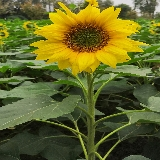
\includegraphics[scale=0.55]{te3.jpg}
      \subcaption{test3}
      \end{minipage}
      \begin{minipage}[t]{0.24\textwidth}
        \centering
        
\includegraphics[scale=0.73]{te4.jpg}
        \subcaption{test4}
        \end{minipage}
   \caption{测试图片}
   \end{figure}
   第三部分所述的六种方案\footnote{方案三基于稀疏编码的SIFT特征算法实现时由于论文细节过少,未能达到预期效果,故而不展示其对应的结果。}对应的缩写为:VCB、FD、SFTA、CNN、TF-CNN和FCN-CNN,本文以后部分均按照这种缩写格式书写,不再另行说明。
   \begin{spacing}{1.25}
    \begin{longtable}[c]{p{0.17\textwidth}p{0.17\textwidth}p{0.17\textwidth}p{0.17\textwidth}p{0.17\textwidth}}
      \caption{图片分类示例}\label{tab:performance}\\
      \toprule[1.5pt]
      图片编号 & 1 & 2 & 3 & 4  \\\midrule[1pt]
      \endfirsthead
      \multicolumn{5}{c}{续表~\thetable\hskip1em 方案二的程序模块说明}\\
      \toprule[1.5pt]
      图片编号 & 1 & 2 & 3 & 4 \\\midrule[1pt]
      \endhead
      \hline
      \multicolumn{5}{r}{续下页}
      \endfoot
      \endlastfoot
      真实标签&Sunflower&Sunflower&Sunflower&Sunflower\\
      \midrule[1pt]
      VCB & Sunflower & Buttercup & Sunflower&Sunflower\\
      FD  & Sunflower &Lilyvalley&Lilyvalley&Sunflower\\
      SFTA & Lilyvalley & Lilyvalley & Sunflower&Sunflower\\
      TF-CNN-VGG16 & Sunflower & Iris & Lilyvalley&Sunflower\\
      TF-CNN-RESNET18 &Buttercup &Buttercup &Buttercup & Buttercup\\
      TF-CNN-INCEPTION-V3 &Buttercup &Iris & Buttercup &Sunflower \\
      TF-CNN-RESNET50 &Buttercup & Buttercup & Buttercup & Windflower\\
      TF-CNN-RESNET101 &Buttercup & Buttercup & Buttercup & Buttercup\\
      \bottomrule[1.5pt]
      \end{longtable}
    \end{spacing}

    可以看出实际拍摄的图片与用于训练的图片有较大的差距,我们拍摄的向日葵的图片,观察给定数据集可知,大部分向日葵图片中花朵处于图片中央且仅有少部分包括绿色的叶子和根茎背景;而拍摄的图片中背景嘈杂,且分割算法对于天空背景的去除效果较差,且花朵均不处于图片中央,其中还有一张图片有多个向日葵花朵,对分类器具有极大的迷惑性。而且训练集过小,深度神经网络十分容易过拟合,所以对目标图片的泛化能力大幅下降。

    对于上述问题,可以对图片作花朵检测,对于框出的花朵区域再进行分类,预期可以获得较好的实验结果。限于时间和能力的限制,包括没有已经标注用于检测的花卉数据集,本次课程设计并没有完成相关工作,后续可以考虑采用迁移学习的方法利用其他的数据集训练的模型迁移到花朵数据集上用于花卉检测。
    \subsection{实验结果及其分析}
    按照课程设计要求,我们将数据集每一类的40张图片作为训练集,其余图片作为测试集,重复实验5次,计算分类正确率的均值和方差。本次课程设计中,我们的分类数据集包括6类分类数据集和102类分类数据集,但是由于102类分类数据集数据量庞大,传统方法计算代价大,所以没有测试。下面分别介绍每一种方案所达到的正确率结果。
    \subsubsection{基于手动特征提取的花卉识别方法}
    方案一是基于视觉词汇提取特征和KNN算法的花卉识别方法,其结果如表4-2所示,表中N-代表没有进行花卉分割,S-代表进行花卉分割;clr-表示使用的是颜色特征,sha-表示使用的是形状特征,tex-表示使用的是纹理特征,all-表示使用的是上述三种特征的混合。
    \begin{spacing}{1.25}
      \begin{longtable}[c]{llllllllll}
        \caption{方案一的实验结果}\label{tab:performance}\\
        \toprule[1.5pt]
        方法 & N-clr & N-sha & N-tex & N-all & S-clr & S-sha & S-tex & S-all  \\\midrule[1pt]
        \endfirsthead
        \multicolumn{9}{c}{续表~\thetable\hskip1em 方案一的实验结果}\\
        \toprule[1.5pt]
        方法 & N-clr & N-sha & N-tex & N-all & S-clr & S-sha & S-tex & S-all  \\\midrule[1pt]
        \endhead
        \hline
        \multicolumn{9}{r}{续下页}
        \endfoot
        \endlastfoot
        均值&31.92&32.42&15.58&29.08&61.5&47.5&30.58&\textbf{64.25}\\
        方差&4.836&1.676&2.306&2.754&2.033&2.571&4.850&3.284\\
        \bottomrule[1.5pt]
        \end{longtable}
      \end{spacing}
    
      可以看出,基于视觉词汇的花卉识别方法中颜色特征的可靠性最高,而形状和纹理特征提取的具有区分性的信息较少,图4-3所示是对提取的颜色、形状和纹理特征的可视化结果,从中可以看出颜色特征的可区分性比形状特征和纹理特征的可区分性高很多。从图4-3中看出Buttercup和Sunflower的颜色特征混杂在一起,因为这两种花的颜色均为黄色,所以仅通过颜色特征无法区分这两种花。
      \begin{figure}[H]
        \begin{minipage}[t]{\textwidth}
        \centering
         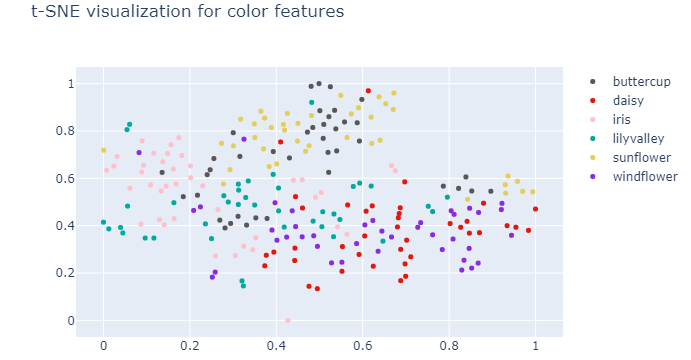
\includegraphics[scale=0.7]{1.png}
         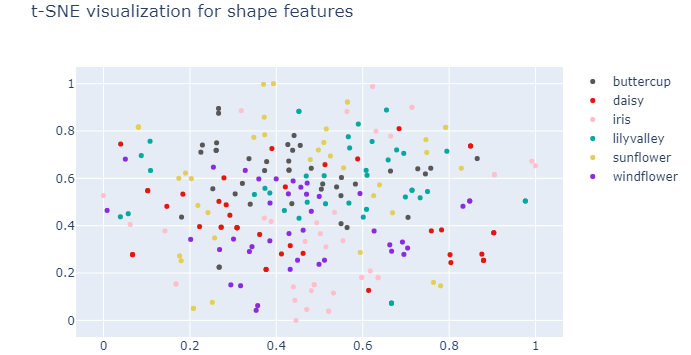
\includegraphics[scale=0.7]{2.png}
         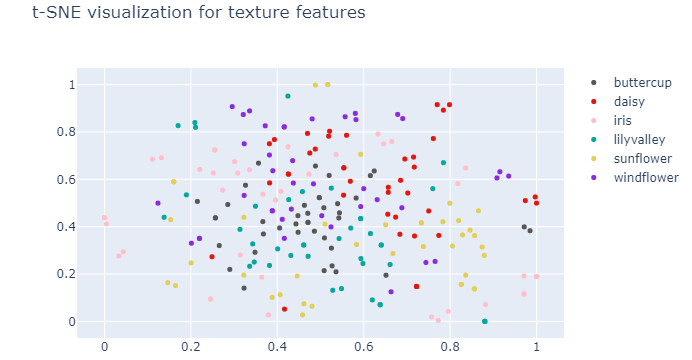
\includegraphics[scale=0.7]{3.png}
         \end{minipage}
       \caption{方案一的数据可视化}
       \end{figure}
      
      通过表4-2中数据可以看出分割算法具有提高分类正确率的效果,去除了背景的干扰可以提高相应任务的分类正确率。正如前文中提到的一样,原有论文中的方法速度较慢,运算代价大,我们将形状和纹理的提取方法做了一定的改变,从结果中可以看出,导致形状和纹理特征对分类效果没有起到积极的作用。

      方案二是基于融合特征的花卉识别方法,图4-4所示是融合特征的花卉识别方法的数据可视化,可以看出由于数据维度较高,t-SNE数据可视化降维到2维可视化时不能完全揭示其可分性,所以从图中看出数据的可分性比方案一中的颜色特征的可分性差。\begin{figure}[H]
        \setlength{\abovecaptionskip}{0.2cm}
        \setlength{\belowcaptionskip}{-0.cm}
          \centering%
          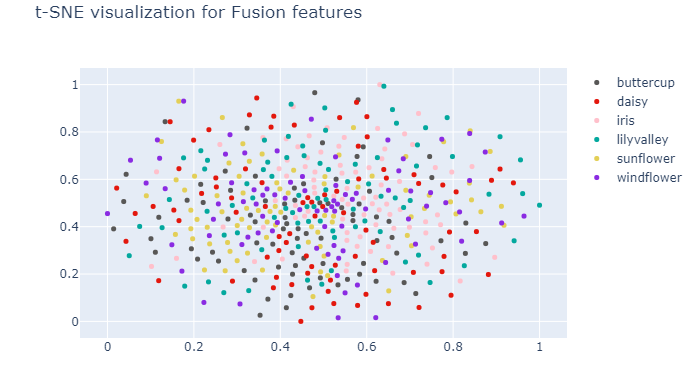
\includegraphics[scale=0.6]{4.png}
          \caption{方案二的数据可视化}
        \end{figure}
      表4-3所示是方案二的分类正确率结果,其中n-表示没有进行图像分割,s-表示进行图像分割;-rbf表示使用RBF核,-hik表示使用HIK核。
      \begin{spacing}{1.25}
        \begin{longtable}[c]{lllll}
          \caption{方案二的实验结果}\label{tab:performance}\\
          \toprule[1.5pt]
          方法 & n-rbf&n-hik&s-rbf&s-hik \\\midrule[1pt]
          \endfirsthead
          \multicolumn{5}{c}{续表~\thetable\hskip1em 方案二的实验结果}\\
          \toprule[1.5pt]
          方法 & n-rbf&n-hik&s-rbf&s-hik \\\midrule[1pt]
          \endhead
          \hline
          \multicolumn{5}{r}{续下页}
          \endfoot
          \endlastfoot
          均值&43.50&56.50&41.33&\textbf{61.17}\\
          方差&3.684&8.713&4.395&4.659\\
          \bottomrule[1.5pt]
          \end{longtable}
        \end{spacing}
      其中s-hik对应的方法表现的最好,其对应的混淆矩阵如图4-5所示,\begin{figure}[H]
        \setlength{\abovecaptionskip}{0.2cm}
        \setlength{\belowcaptionskip}{-0.cm}
          \centering%
          \includegraphics[scale=0.4]{5.png}
          \caption{方案二的混淆矩阵(s-hik)}
        \end{figure}
      可以看出,将Buttercup错分为windflower的可能性较高,Sunflower正确分类的概率最高。

      方案四是基于SFTA特征的花卉识别方法,图4-6所示是SFTA特征的数据可视化,\begin{figure}[H]
        \setlength{\abovecaptionskip}{0.2cm}
        \setlength{\belowcaptionskip}{-0.cm}
          \centering%
          \includegraphics[scale=0.6]{6.png}
          \caption{方案四的数据可视化}
        \end{figure}
      
      方案四采用决策树、随机森林和支持向量机三种分类算法,其正确率如表4-4所示,其中DT表示决策树(Decision Tree),RF表示随机森林(Random Forest),SVM表示支持向量机(Support Vector Machine)。
      \begin{spacing}{1.25}
        \begin{longtable}[c]{llll}
          \caption{方案四的实验结果}\label{tab:performance}\\
          \toprule[1.5pt]
          方法 & SFTA-DT&SFTA-RF&SFTA-SVM \\\midrule[1pt]
          \endfirsthead
          \multicolumn{4}{c}{续表~\thetable\hskip1em 方案四的实验结果}\\
          \toprule[1.5pt]
          方法 & SFTA-DT&SFTA-RF&SFTA-SVM \\\midrule[1pt]
          \endhead
          \hline
          \multicolumn{4}{r}{续下页}
          \endfoot
          \endlastfoot
          均值&41.67&\textbf{55.83}&55.42\\
          方差&3.684&2.713&3.395\\
          \bottomrule[1.5pt]
          \end{longtable}
        \end{spacing}
      可以看出基于SFTA特征的随机森林方法的分类效果最好,图4-7所示分别对应上述三种方法的混淆矩阵,\begin{figure}[H]
        \begin{minipage}[t]{0.32\textwidth}
        \centering
         \includegraphics[scale=0.22]{7.png}
         \subcaption{决策树的混淆矩阵}
         \end{minipage}
         \begin{minipage}[t]{0.32\textwidth}
         \centering
         \includegraphics[scale=0.22]{8.png}
         \subcaption{随机森林的混淆矩阵}
         \end{minipage}
         \begin{minipage}[t]{0.32\textwidth}
          \centering
          \includegraphics[scale=0.22]{9.png}
          \subcaption{支持向量机的混淆矩阵}
          \end{minipage}
       \caption{方案四的分类混淆矩阵}
       \end{figure}

       从中可以看出,对于SFTA特征,随机森林分类算法的可区分性最高,其与决策树进行比较,可以看出集成学习的作用,通过集成几个弱分类器来提高分类器性能。
      \subsubsection{深度学习方法}
      本次课程设计中,除了测试了一种简单的卷积神经网络模型,我们主要采用了基于迁移学习的卷积神经网络模型并取得良好的分类正确率和稳定性,主要包含VGG16、Inception-v3、RESNET18、RESNET50和RESNET101五种常用的图像识别模型,表4-5和表4-6分别是上述五种模型在6类分类数据集和Oxford-102数据集上的结果。
      \begin{spacing}{1.25}
        \begin{longtable}[c]{llllll}
          \caption{卷积神经网络在6分类数据集上的结果}\label{tab:performance}\\
          \toprule[1.5pt]
          方法 & VGG16 & INCEPTION-V3 & RESNET18 & RESNET50 & RESNET101 \\\midrule[1pt]
          \endfirsthead
          \multicolumn{6}{c}{续表~\thetable\hskip1em 卷积神经网络在6分类数据集上的结果}\\
          \toprule[1.5pt]
          方法 & VGG16 & INCEPTION-V3 & RESNET18 & RESNET50 & RESNET101 \\\midrule[1pt]
          \endhead
          \hline
          \multicolumn{6}{r}{续下页}
          \endfoot
          \endlastfoot
          均值&75.58&84.58&90.92&93.00&\textbf{95.17}\\
          方差&2.482&1.264&0.311&0.310&0.206\\
          \bottomrule[1.5pt]
          \end{longtable}
        \end{spacing}
        \begin{spacing}{1.25}
          \begin{longtable}[c]{llllll}
            \caption{卷积神经网络在Oxford 102数据集上的结果}\label{tab:performance}\\
            \toprule[1.5pt]
            方法 & VGG16 & INCEPTION-V3 & RESNET18 & RESNET50 & RESNET101 \\\midrule[1pt]
            \endfirsthead
            \multicolumn{6}{c}{续表~\thetable\hskip1em 卷积神经网络在Oxford 102数据集上的结果}\\
            \toprule[1.5pt]
            方法 & VGG16 & INCEPTION-V3 & RESNET18 & RESNET50 & RESNET101 \\\midrule[1pt]
            \endhead
            \hline
            \multicolumn{6}{r}{续下页}
            \endfoot
            \endlastfoot
            均值&49.62&64.53&72.48&75.69&\textbf{76.08}\\
            方差&0.780&0.447&0.633&0.567&0.448\\
            \bottomrule[1.5pt]
            \end{longtable}
          \end{spacing}

        为了对比手动提取特征的方法(方案一、二、三和四)和深度学习方法,我们尝试提取网络中的一些数据作为提取的花卉的特征,将数据作为二维图像可视化来进行比较分析。

        我们以Inception-V3这一模型的输出结果为例来进行进一步的分析。由于靠前的层数的数据不具有直观性且数据庞大,那么我们选择用最后的全连接层的数据($2048\times 1$)作为神经网络所提取的特征。相当于每一幅图像都有一个2048维度的特征向量。那么为了更加直观的分析,我们采用t-SNE的方法,将特征维度降低到2,可以在二维平面中直观地观察到结果。相对于手动提取的特征,很明显神经网络模型提取的特征的可分性要好得多。从最终的结果也可以看出来,对于六种花卉的识别率可以达到将近百分八十五,相对于之前的算法的特征要好很多。

        如图4-8(a)所示是Inception-V3模型提取特征的可视化,图4-8(b)是将得到的特征放入SVM分类器中分类得到的混淆矩阵。
        \begin{figure}[H]
            \setlength{\abovecaptionskip}{0.2cm}
            \setlength{\belowcaptionskip}{-0.2cm}
            \centering%
            \subcaptionbox{Inception-V3的特征可视化} %标题的长度,超过则会换行,如下一个小图。
              {\includegraphics[height=5cm]{10.png}}%
            \hspace{2em}%
            \subcaptionbox{Inception-V3的特征用SVM分类的混淆矩阵}
                {\includegraphics[height=5cm]{11.png}}
          
            \caption{Inception-V3模型的特征可视化分析}
            \end{figure}
        从上图中我们可以很清楚地看出,Livyvalley和其他花朵相对来说和其他没有什么重叠,得到的准确率比较高。我们分析可能是他的颜色形状和其他的很不一样,相对于其他花朵图片都是一朵大花,Livyvalley是一串小花。其次是百分之八十五正确率的Daisy,相对于其他类型花朵的图片,这组图片花朵拍摄清晰,花朵均为正面拍摄,且花朵均为白色,肉眼可见这组图片中的花朵都较为相似,所以得到的结果也会更好。Buttercup的准确分辨率最低,也就是这样得出的特征这种花是最差的,从可视化图片中也可以看出来相应的颜色小点也是最为分散的一组。我们分析原因是Buttercup中花朵的形状有正面也有侧面,花朵在照片中的占比不同,而且各种花朵拍照的光线差距较大,即总体形态相差较大。Buttercup和Iris互相之间分别均有百分之二十的错误率。Iris之中有各种各样颜色的花朵,其中黄色的花朵和Buttercup之中的花朵比较相似,而同为黄色花朵的Sunflower正确率较高,是由于其花朵的形态和其他区别较大。而Iris这种的花朵的分类结果差很大程度是由于这种花的颜色变化很多,结合之前的实验可以得到一个结果就是花朵的颜色在花朵分类之中占据了很大的比例。Windflower有一大半是集中的,一小半是掺杂在其他类中,也和结果的百分之六十八比较吻合。分析相对来说其中只有一朵花且花朵较大的图片分类正确几率更高。而Sunflower的错误分类在二维特征中很难解释,除开黄色和其他有一定相似,这一种花朵形状完全不一致,按照预期推测可能会有更高的正确率,推测是因为直观观察采用的降维方法引起的信息丢失,可能相对在更高维度来说他们可以被更好的区分开来。有一个比较突出的问题就是对于一张照片中存在多株花朵的情况,这一种的分类效果就会下降很多。分析是由于模型无法分辨有几朵花朵,对花朵进行特征提取的时候就会受到花朵数量的影响,无法正确地提取一朵花朵的信息。相应的我们有想法先对所有图片进行单株花朵级别的图像分割,即保证每个输入的图片都是一朵花朵,但最后没有成功,但是这是一个可以进一步研究的方向。

        另外我们尝试将未分割的花朵图片直接进行分类。很有趣的一个点是对于所给的六种花朵的分类(每张图片中都只有一朵花),在深度学习的模型中,背景对于花卉的分类效果的影响变得很小。我们思考是在这样的一个模型之中,已经起到了一个对花卉图片的分割的效果。

        进一步采用更复杂的模型,如RESNET101模型,得到的正确率可以高达百分之九十五(见表4-5)。我们尝试对其中提取的特征进行进一步的物理等实际意义上的分析,但是都以失败告终,未能得出有效结论。

        当我们尝试进行更高更复杂的分类,如Oxford102数据集,卷积神经网络也可以达到一个较为良好的效果。正确率最高的为RESNET101模型,正确率也在百分之七十六以上。而对于如此复杂的数据集,受限于我们的相关专业知识,以手动提取特征的方法我们已经无能为力了。
  \section{总结与展望}
  本次课程设计我们选择的题目是基于图像的花卉识别。花卉识别是一个具有较高挑战性的问题,我们在选题时因其看起来目标清晰明了、数据集不是很庞大,认为该题目比较容易上手所以选定此题。在接触问题的初期,我们调研了相关文献,发现问题的难度超过了我们的预期。花卉识别的难点很多,比如自然界中的花朵种类很多,有些不同种的花朵长相十分相似,资深的植物学家可能都有误判的时候;而且同一种花在不同的生长周期会呈现出不同形态,对分类造成很大干扰。而且一般植物学家判断一朵花的种类,往往不仅仅依赖花朵的外观,包括其生长的地理位置、潮湿程度等等周围环境因素来综合判断该花的种类,所以基于图像的花卉识别理论上也存在一定的误判概率。

  通过前期的调研,我们初步确定了7种解决方案,主要分为非深度学习方法和深度学习方法两大类。非深度学习方法主要的难点在于如何提取到优质的特征能够特异地表示每一类花卉;而深度学习方法主要的难点集中在如何确定网络结构。在本次课程设计中,我们将深度学习与迁移学习相结合,借助已有网络模型在ImageNet上的训练参数,大大减少了我们训练所需花费的时间和缓解了我们数据集过小的困境。

  在编写代码的过程中,我们发现将论文中方法转换为实际的程序并能够达到论文宣称的结果是具有难度的。尤其是在非深度学习方法中,例如前文我们采用的方案一中的方法,提取图像的颜色、形状和纹理特征,采用k-means聚类对把图像中每一个像素点当作一个数据点进行聚类,通常一幅图像的像素点的数量就是十万数量级,所以程序十分耗时且基本上无法在我们自己的电脑上跑完。于是我们对图像的数据进行压缩,保留基本信息的同时削减数据量,从而加快程序运行的速度。但是我们最终并没有达到论文中的实验效果,可能也跟这里有很大关系。当然,由于论文叙述的大部分是原理,实际操作过程中的一些论文作者自己的细节操作并没有公布出来,可能也是造成我们无法实现论文中的结果的一个很大的因素。

  在我们进行论文调研的时候,发现花卉分类还有一个常见的情形:就是在自然界中我们还能发现我们从未发现的新的花卉品种,我们如何通过机器学习方法自动识别出这是一种新的花卉,或者这种并未出现在训练的数据集中,但应用场景中却经常出现,并且我们掌握这种花的一些性状或者属性描述。这里所提到的就是Zero-shot Learning。零样本学习或者少样本学习是当前机器学习领域中比较热门的分支,其能解决的场合十分普遍。但是在本次课程设计中,由于缺乏带属性标注的数据集,我们并没有相关方面的实质性的工作。

  在花卉识别之前,首先要对花卉图像进行分割处理,本次课程设计中我们采用了几种常见的花卉分割方法。但是在面对一幅图像中有多个花朵,即包含多个目标时,如何将其逐个分割出来就成为新的挑战。通过中期验收与老师的沟通,我们得知可以通过一些特殊的神经网络来完成上述问题,如mask-RCNN。但是由于缺乏已标注的分割数据集且找不到已训练好的网络模型参数\footnote{tensorflow中包含这种模型,但由于网络原因没有完成下载。},我们同样未能完成上述工作,希望可以在以后的工作学习中可以有相关工作的尝试。

  通过本次课程设计的实践,我们了解到一个模式识别的问题应该如何被分析和解决,对于科研工作有了一定的初步了解,从查阅文献到复现代码,通过不断的尝试和老师师兄的指导,一步一步逐渐地完成课程设计的任务,让我们收获颇丰。
	%生成参考文献
  %使用方法:\bibliography{参考文件1文件名, 参考文献2文件名, ...}
	\bibliography{Bibs/mybib}
	
  \begin{appendices}
    \section{补充的图像处理知识}
    \subsection{SIFT特征提取算子}
    SIFT特征是Scale Invariant Feature Transform的缩写,由加拿大教授David G.Lowe提出。SIFT特征对旋转、尺度缩放、亮度变化等保持不变性,是一种非常稳定的局部特征。

    {\heiti  多分辨率图像金字塔:}在早期图像的多尺度通常使用图像金字塔表示形式。图像金字塔是同一图像在不同的分辨率下得到的一组结果,其生成过程一般包括两个步骤:\begin{itemize}
     \item  对原始图像进行平滑;
     \item 对处理后的图像进行下采样,下采样后得到一系列尺寸不断缩小的图像。
    \end{itemize}

    {\heiti  高斯尺度空间:}我们还可以通过图像的模糊程度来模拟人在距离物体由远到近时物体在视网膜上成像过程,距离物体越近其尺寸越大图像也越模糊,这就是高斯尺度空间。使用不同的参数模糊图像(分辨率不变),时尺度空间的另一种表现形式。我们知道图像和高斯函数进行卷积运算能够对图像进行模糊,使用不同的高斯核可得到不同模糊程度的图像。一幅图像其高斯尺度空间可由其和不同的高斯卷积得到:\begin{gather}
      L(x,y,\sigma)=G(x,y,\sigma)*I(x,y)\\
      G(x,y,\sigma)=\dfrac{1}{2\pi\sigma^2}e^{\frac{x^2+y^2}{2\sigma^2}}
    \end{gather}
    其中,$G(x,y,\sigma)$时高斯核函数,$\sigma$成为尺度空间因子,它是高斯正态分布的标准差,反映了图像被模糊的程度,其值越大图像越模糊,对应的尺度也就越大。$L(x,y,\sigma)$代表着图像的高斯尺度空间。构建尺度空间的目的是为了检测不同的尺度下都存在的特征点,而检测特征点较好的算子时高斯拉普拉斯算子,\begin{gather}
      \Delta^2=\dfrac{\partial^2}{\partial x^2}+\dfrac{\partial^2}{\partial y^2}
    \end{gather}
    使用高斯拉普拉斯算子虽然能够较好的检测到图像中的特征点,但是其运算量过大,通常可以使用差分高斯(Difference of Gaussia, DOG)来近似计算。设$k$为相邻两个高斯尺度空间的比例因子,则DoG的定义为\begin{gather}
     D(x,y,\sigma)=[G(x,y,k\sigma)-G(x,y,\sigma)]*I(x,y)=L(x,y,k\sigma)-L(x,y,\sigma)
    \end{gather}
    其中,$L(x,y,\sigma)$是图像的高斯尺度空间。从上式可以知道,将相邻的两个高斯空间的图像相减就得到了DoG的响应图像。为了得到DoG图像,先要构建高斯尺度空间,而高斯的尺度空间可以在图像金字塔降采样的基础上加上高斯滤波得到,也就是对图像金字塔的每层图像使用不同的参数$\sigma$进行高斯模糊,使每层金字塔有多张高斯模糊过的图像。降采样时,金字塔上边一组图像的第一张是由其下面一组图像倒数第三张采样得到的。

    易知,高斯金字塔有多组,每组又有多层。一组中的多个层之间的尺度是不一样的,相邻两层之间的尺度相差一个比例因子$k$。高斯金字塔构建完成后,将相邻的高斯金字塔相减就得到了DoG金字塔。高斯金字塔的组数一般是\begin{gather}
      o=[\log_2\min(m,n)]-a
    \end{gather}
    其中$o$表示金字塔的层数,$m,n$分别是图像的行和列。减去的系数$a$可以在$0\sim\log_2\min(m,n)$之间的任意值。高斯模糊参数$\sigma$可由下式得到\begin{gather}
      \sigma(o,s)=\sigma_02^{\frac{o+s}{S}}
    \end{gather}
    其中$o$为所在的组,$s$为所在的层,$\sigma_0$为初始的尺度,$S$为每组的层数。

    {\heiti  DoG空间极值检测:}为了寻找尺度空间的极值点,每个像素点要和其图像域(同一尺度空间)和尺度域(相邻的尺度空间)的所有相邻点进行比较,当其大于(或者小于)所有相邻点时,该点就是极值点。

    {\heiti  删除不好的极值点:}通过比较检测得到的DoG的局部极值点是在离散空间搜索得到的,由于离散空间是对连续空间采样得到的结果,因此在离散空间找到的极值点不一定是真正意义上的极值点,因此要设法将不满足条件的点剔除掉。可以通过尺度空间DoG函数进行曲线拟合寻找极值点,这一步的本质是去掉DoG局部曲率非常不对称的点。要剔除掉的不符合要求的点主要有两种:低对比度的特征点和不稳定的边缘响应点。

    {\heiti 剔除低对比度的特征点:}对于候选特征点$x$,其偏移量定义为$\Delta x$,其对比度为$D(x)$的绝对值$\lvert D(x) \rvert$,对$D(x)$应用泰勒展开式\begin{gather}
      D(x)=D+\dfrac{\partial D^T}{\partial x}\Delta x+\dfrac{1}{2}\Delta x^T\dfrac{\partial^2 D}{\partial x^2}\Delta x\\
      \Delta x=-\dfrac{\partial^2 D^{-1}}{\partial x^2}\dfrac{\partial D(x)}{\partial x}
    \end{gather}
    
    由于$x$是$D(x)$的极值点,所以对上式求导并令其为0,得到\begin{gather}
      D(\hat{x})=D+\dfrac{1}{2}\dfrac{\partial D^T}{\partial x}\hat{x}
    \end{gather}

    然后再把求得的$\Delta x$代入到$D(x)$的泰勒展开式中。设对比度的阈值为$T$,若$\lvert D(\hat{x}) \rvert\geq T$,则该特征点保留,否则剔除掉。

    {\heiti 剔除不稳定的边缘响应点:}在边缘梯度的方向上主曲率值比较大,而沿着边缘方向则主曲率值比较小。候选特征点的DoG函数$D(x)$的主曲率与$2\times 2$的Hessian矩阵$H$的特征值成正比,\begin{gather}
     H=\begin{bmatrix}
        D_{xx}&D_{yx}\\
        D_{xy}&D_{yy}
     \end{bmatrix}
    \end{gather}
    其中$D_{xx},D_{xy}=D_{yx},D_{yy}$是候选点邻域对应位置的差分求得的。设$\alpha=\lambda_{\text{max}}$为$H$的最大特征值,$\beta=\lambda_{\text{min}}$为其最小特征值,则\begin{gather}
      \text{Tr}(H)=D_{xx}+D_{yy}=\alpha+\beta\\
      \text{Det}(H)=D_{xx}+D_{yy}-D^2_{xy}=\alpha\beta
    \end{gather}
    
    设$\gamma=\alpha/\beta$表示最大特征值和最小特征值的比值,则\begin{gather}
     \dfrac{\text{Tr}(H)^2}{\text{Det}(H)}=\dfrac{(\alpha+\beta)^2}{\alpha\beta}=\dfrac{(\gamma\beta+\beta)^2}{\gamma\beta^2}=\dfrac{(\gamma+1)^2}{\gamma}
    \end{gather}

    因此,为了检测主曲率是否在某个阈值$T_{\gamma}$下,只需检测\begin{gather}
      \dfrac{\text{Tr}(H)^2}{\text{Det}(H)}>\dfrac{(T_{\gamma}+1)^2}{T_{\gamma}}
    \end{gather}

    {\heiti  求取特征点的主方向:}经过上面的步骤已经找到了在不同尺度下都存在的特征点,为了实现图像旋转不变性,需要给特征点的方向进行赋值。利用特征点邻域像素的梯度分布特性来确定其方向参数,再利用图像的梯度直方图求取关键局部结构的稳定方向。

    找到了特征点,也就可以得到该特征点的尺度$\sigma$,也就可以得到特征点所在的尺度图像\begin{gather}
     L(x,y)=G(x,y,\sigma)*I(x,y)
    \end{gather}

    计算以特征点为中心,以$3\times 1.5\sigma$为半径的区域图像的辐角和幅值,每个点的$L(x,y)$的梯度的模$m(x,y)$以及方向$\theta(x,y)$可通过下式求得\begin{gather}
      m(x,y)=\sqrt{[L(x+1,y)-L(x-1,y)]^2+[L(x,y+1)-L(x,y-1)]^2}\\
      \theta(x,y)=\text{arctan}\dfrac{L(x,y+1)-L(x,y-1)}{L(x+1,y)-L(x-1,y)}
    \end{gather}

    得到特征点的主方向后,对于每个特征点可以得到三个信息$(x,y,\theta)$,即位置、尺度和方向。由此可以确定一个SIFT特征区域,一个SIFT特征区域由三个值表示,中心表示特征点位置,半径表示关键点的尺度,箭头表示主方向。具有多个方向的关键点可以被复制成多份,然后将方向值分别赋给复制后的特征点,一个特征点就产生了多个坐标、尺度相等,但是方向不同的特征点。

    {\heiti  生成特征描述:}校正旋转主方向,确保旋转不变性;生成描述子,最终形成一个128维的特征向量;归一化处理,将特征向量长度进行归一化处理,进一步去除光照的影响。
    \subsection{LBP算子}
    LBP是Local Binary Pattern的缩写,译为局部二值模式,是一种用来描述图像局部特征的算子。LBP特征具有灰度不变性和旋转不变性等显著优点。它是由T.Ojala,M.Pietikainen和D.Harwood在1994年提出的。由于LBP特征计算简单、效果较好,因此LBP特征在计算机视觉的许多领域都得到了广泛的应用,LBP特征比较出名的是应用在人脸识别和目标检测中,在计算机视觉来源库OpenCV中有使用LBP特征进行人脸识别的接口,也有用LBP特征训练目标检测分类器的方法。

    原始LBP特征定义在像素3*3的邻域内,以邻域中心像素为阈值,相邻的8个像素的灰度值与邻域中心的像素值进行比较,若周围像素大于中心像素值,则该像素点的位置被标记为1,否则为0。上述过程可表示为\begin{gather}
     LBP(x_c,y_c)=\sum\limits_{p=0}^{P-1}2^{p}s(i_p-i_c)
    \end{gather}
    其中$i_c$表示中心像素$(x_c,y_c)$的像素值,$i_n$表示其近邻像素的像素值,函数$s$为\begin{gather}
      s(x)=\left\{
       \begin{array}{ll}
         1&\text{if  }x\geq0\\
         0&\text{else}
       \end{array}
      \right.
    \end{gather}

    后来将LBP从定义在固定邻域上转变为定义在固定半径范围内的小区域,改进后的LBP算子允许在半径为$R$的圆形邻域内有任意多个像素点,经过采样得到含有$P$个采样点的LBP算子。LBP的主要步骤如下:\begin{itemize}
    \item  将检测窗口划分为固定大小的小区域(cell);
    \item 对于每个cell中的每一个像素,将其指定邻域的采样点的像素的灰度值与其进行比较,若采样点像素值大于中心像素值,则该像素点的位置标记为1,否则为0;
    \item 然后计算每个cell的直方图,对该直方图进行归一化处理;
    \item 最后将得到的每一cell的统计直方图连接成一个特征向量,也就是整幅图的LBP纹理特征向量。
    \end{itemize}
    \subsection{Canny算子}
    Canny提出一种新的边缘检测方法,它对受白噪声影响的阶跃型边缘是最优的。Canny检测子的最优性与三个标准有关:第一,检测标准,不失去重要的边缘,不应有虚假的边缘;第二,定位标准,实际边缘与检测到的边缘位置之间的偏差最小;第三,单位应标准,将多个响应降低为单个边缘响应。这一点被第一个标准部分地覆盖了。这第三个标准解决受噪声影响地边缘问题,起抑制非平滑边缘检测算子的作用。

    Canny提出了特征综合方法。首先标记处所有由最小尺度算子得到的突出边缘。而整个Canny边缘检测器算法分成如下四步:\begin{itemize}
      \item  噪声去除。因为这个检测器用到了微分算子,所以对于局部的不连续是敏感的,某区域的噪声点很容易造成边缘的模糊;
      \item 计算图像梯度,得到可能边缘;
      \item 非最大梯度值抑制。通常灰度变化的地方都比较集中,将局部范围内的梯度方向上,灰度变化最大的保留下来,其它的不保留,这样可以剔除掉一大部分的点。将由多个像素宽的边缘变成一个单像素宽的边缘;
      \item 双阈值筛选。通过给非极大值抑制后,仍然有很多的可能边缘点,进一步的的设置一个双阈值,即低阈值和高阈值。灰度变化大于高阈值的,设为强边缘像素;低于低阈值的,剔除。在低阈值和高阈值之间的设置为弱边缘。进一步判断,如果其领域内有强边缘像素,保留,如果没有,剔除。
    \end{itemize}
    \section{神经网络简介}
    \subsection{神经网络概述}
    人工神经网络中最小也最重要的单元叫神经元。与生物神经系统类似,这些神经元也互相连接并具有强大的处理能力。一般而言,人工神经网络试图复现真实大脑的行为和过程。

    每个神经元都有输入连接和输出连接。这些连接模拟了大脑中突触的行为。与大脑中突触传递信号的方式相同——信号从一个神经元传递到另一个神经元,这些连接也在人造神经元之间传递信息。每一个连接都有权重,这意味着发送到每个连接的值要乘以这个因子。这种模式是从大脑突触得到的启发,权重实际上模拟了生物神经元之间传递的神经递质的数量。所以,如果某个连接重要,那么它将具有比那些不重要的连接更大的权重值。\begin{figure}[H]
      \setlength{\abovecaptionskip}{0.2cm}
      \setlength{\belowcaptionskip}{-0.2cm}
      \centering%
      \subcaptionbox{单个神经元的模型} %标题的长度,超过则会换行,如下一个小图。
        {\includegraphics[height=4cm]{20.jpg}}%
      \hspace{2em}%
      \subcaptionbox{人工神经网络的结构模型}
          {\includegraphics[height=4cm]{21.jpg}}
      \caption{神经网络}
      \end{figure}
    由于可能有许多值进入一个神经元,每个神经元便有一个所谓的输入函数。通常,连接的输入值都会被加权求和。然后该值被传递给激活函数,激活函数的作用是计算出是否将一些信号发送到该神经元的输出。
    \subsection{反向传播算法}
    根据梯度下降法,我们在每一次迭代过程中都会按照下式进行参数更新,\begin{gather}
      W^{(l)}_{ij}=W^(l)_{ij}-\eta\dfrac{\partial}{\partial W^{(l)}_{ij}}J(W,b)\\
      b^{(l)}_{i}=b^{(l)}_{i}-\eta\dfrac{\partial}{\partial b^{(l)}_{i}}J(W,b)
    \end{gather}
    其中$\eta$是初始学习率。

    反向传播算法的思路如下:给定一个样例$(x,y)$,我们首先进行“前向传导”运算,计算出网络中所有的激活值,包括$h_{W,b}(x)$的输出值。之后,针对第$l$层的每一个节点$i$,我们计算出其残差$\delta^{(l)}_i$,该残差表明了该节点对最终输出值的残差产生了多少影响。对于最终的输出节点,我们可以直接计算出网络产生的激活值与实际值之间的差距,我们将这个差距定义为$\delta^{(n_l)}_i$为输出层的残差。下面给出关于输出层和隐藏层的残差计算公式:\begin{gather}
     \delta^{n_l}_i=\dfrac{\partial}{\partial z_i^{n_l}}\dfrac{1}{2}\lVert y-h_{W,b}(x)\rVert^2=-(y_i-a^{(n_l)}_i)f'(z^{(n_l)}_i)\\
     \delta^{(l)}_i=\left( \sum\limits^{s_{l+1}}_{j=1}W^{(l)}_{ji}\delta^{(l+1)}_j \right)f'(z^{(l)}_i)
    \end{gather}

    那么,反向传播算法可表示为以下几个步骤:\begin{itemize}
     \item 进行前馈传导计算,利用前向传导公式,得到$L_2,L_3,\dots,L_{n_l}$的输出值;
     \item 对输出层(第$n_l$层),计算\begin{gather}
       \delta^{(n_l)}=-(y-a^{(n_l)})f'(z^{(n_l)})
     \end{gather}
     \item  对于$l=n_l-1,n_l-2,\dots,2$的各层,计算\begin{gather}
      \delta^{(l)}=((W^{(l)})^T\delta^{(l+1)})f'(z^{(l)})
     \end{gather}
     \item  计算最终需要的偏导数值:\begin{gather}
        \nabla_{W^{(l)}}J(W,b;x,y)=\delta^{(l+1)}(a^{(l)})^T\\
        \nabla_{b^{(l)}}J(W,b;x,y)=\delta^{(l+1)}
     \end{gather}
     \item  计算:\begin{gather}
       \Delta W^{(l)}=\Delta W^{(l)}+\nabla_{W^{(l)}}J(W,b;x,y)\\
       \Delta b^{(l)}=\Delta b^{(l)}+\nabla_{b^{(l)}}J(W,b;x,y)
     \end{gather}
     \item  更新权重参数:\begin{gather}
       W^{(l)}=W^{(l)}-\eta\left[ \left( \dfrac{1}{m}\Delta W^{(l)} \right)+\lambda W^{(l)} \right]\\
       b^{(l)}=b^{(l)}-\eta\left[\dfrac{1}{m}\Delta b^{(l)} \right]
     \end{gather}
    \end{itemize}
	  \section{代码}
    \subsection{文件夹:test}
    \textbf{main.py}
    \begin{spacing}{1.25}
		\begin{lstlisting}[language=python]
      """
      方案一:基于视觉词汇的花卉识别方法
      """
      import glob
      import cv2
      import numpy as np
      import pandas as pd
      import matplotlib.pyplot as plt
      import math
      import matplotlib.mlab as mlab
      from sklearn.cluster import KMeans,MiniBatchKMeans
      import kNN
      from mpl_toolkits.mplot3d import Axes3D
      from matplotlib.ticker import NullFormatter
      from sklearn import manifold,datasets
      import utils
      import kNN
      #import afkmc2.afkmc2 as afk
      #import MR8
      from skimage.transform import rotate
      from skimage.feature import local_binary_pattern
      from skimage import data,io,data_dir,filters,feature
      from skimage.color import label2rgb
      import skimage
      from PIL import Image
      import dataLoad
      
      CHOSEN_TRAIN=40#定义每一类选择的训练样本个数
      RADIUS=4#定义LBP算子的区域半径
      N_POINTS=8*RADIUS#定义LBP算子的区域采样点个数
      ALPHA=6.0#颜色特征的权重
      BETA=4.5#形状特征的权重
      GAMMA=3.1#纹理特征的权重
      
      randomIndex,resIndex=dataLoad.randomSample(80,CHOSEN_TRAIN)#随机选取训练样本和测试样本
      filenames=[]
      filenames.append(glob.glob(r'F:/seven/prDesign/fdata/buttercup/*.jpg'))
      filenames.append(glob.glob(r'F:/seven/prDesign/fdata/daisy/*.jpg'))
      filenames.append(glob.glob(r'F:/seven/prDesign/fdata/iris/*.jpg'))
      filenames.append(glob.glob(r'F:/seven/prDesign/fdata/lilyvalley/*.jpg'))
      filenames.append(glob.glob(r'F:/seven/prDesign/fdata/sunflower/*.jpg'))
      filenames.append(glob.glob(r'F:/seven/prDesign/fdata/windflower/*.jpg'))
      #提取原始特征
      dataX,numX=dataLoad.load(filenames,randomIndex,'color',CHOSEN_TRAIN,N_POINTS,RADIUS)
      print('color completed')
      dataY,numY=dataLoad.load(filenames,randomIndex,'shape',CHOSEN_TRAIN,N_POINTS,RADIUS)
      print('shape completed')
      dataZ,numZ=dataLoad.load(filenames,randomIndex,'texture',CHOSEN_TRAIN,N_POINTS,RADIUS)
      print('texture completed')
      #生成类别标签
      y=None
      for i in range(6):
          tempY=(i+1)*np.ones(CHOSEN_TRAIN,dtype=int)
          if y is None:
              y=tempY
          else:
              y=np.concatenate((y,tempY),axis=0)
      
      #聚类生成视觉词汇
      kmeansX=MiniBatchKMeans(n_clusters=200)
      kmeansX.fit(dataX)
      print('color k-means completed')
      
      kmeansY=MiniBatchKMeans(n_clusters=200)
      kmeansY.fit(dataY)
      print('shape k-means completed')
      
      kmeansZ=MiniBatchKMeans(n_clusters=200)
      kmeansZ.fit(dataZ)
      print('texture k-means completed')
      print('k-means complete!')
      centersX,labelsX=kmeansX.cluster_centers_,kmeansX.labels_
      centersY,labelsY=kmeansY.cluster_centers_,kmeansY.labels_
      centersZ,labelsZ=kmeansZ.cluster_centers_,kmeansZ.labels_
      
      #生成最终的特征表达,即用最近邻法统计直方图
      histDataX=np.zeros((6*CHOSEN_TRAIN,200),dtype=int)
      histDataY=np.zeros((6*CHOSEN_TRAIN,200),dtype=int)
      histDataZ=np.zeros((6*CHOSEN_TRAIN,200),dtype=int)
      k=0
      sumXZ=0
      sumY=0
      for filename in filenames:
          for i in range(CHOSEN_TRAIN):
              tempImg=cv2.cvtColor(cv2.imread(filename[i],cv2.IMREAD_COLOR),cv2.COLOR_BGR2HSV)        #m,n,_=tempImg.shape
              m,n,_=tempImg.shape
              for j in range(m+n):
                  histDataX[k*CHOSEN_TRAIN+i,labelsX[j+sumXZ]]=histDataX[k*CHOSEN_TRAIN+i,labelsX[j+sumXZ]]+1
                  histDataZ[k*CHOSEN_TRAIN+i,labelsZ[j+sumXZ]]=histDataZ[k*CHOSEN_TRAIN+i,labelsZ[j+sumXZ]]+1
              for j in range(numY[k*CHOSEN_TRAIN+i]):
                  histDataY[k * CHOSEN_TRAIN + i, labelsY[j + sumY]] = histDataY[k * CHOSEN_TRAIN + i, labelsY[j + sumY]] + 1
              sumXZ=sumXZ+m+n
              sumY=sumY+numY[k*CHOSEN_TRAIN+i]
          k=k+1
      
      
      """
      #使用t-SNE数据可视化
      tsne=manifold.TSNE(n_components=2,init='pca',random_state=0)
      Y=tsne.fit_transform(histData)
      print('tSNE completed!')
      fig=utils.plot_embedding(Y,y,'t-SNE embedding of the digits')
      plt.show()
      """
      #测试,并计算正确率
      """
      sum=0
      t=0
      for filename in filenames:
          t=t+1
          for i in range(CHOSEN_TRAIN,80):
              resultTT=np.zeros(7,dtype=float)
              testFile=filename[resIndex[i-CHOSEN_TRAIN]]
              histTestX=kNN.featureCOV(centersX,testFile)
              histTestY=kNN.featureSIFT(centersY,testFile)
              histTestZ=kNN.featureLBP(centersZ,testFile,N_POINTS,RADIUS)
              print('featuren construction completed!')
              resultC,probC=kNN.xkNN(histDataX,y,histTestX)
              resultS,probS=kNN.xkNN(histDataY,y,histTestY)
              resultT,probT=kNN.xkNN(histDataZ,y,histTestZ)
              resultTT[resultC]=resultTT[resultC]+ALPHA*probC
              resultTT[resultS]=resultTT[resultS]+BETA*probS
              resultTT[resultT]=resultTT[resultT]+GAMMA*probT
              result=np.where(resultTT==np.max(resultTT))
              result=result[0]
              print(resultTT,result,t)
              if result==t:
                  sum=sum+1
      print(sum*100/240)
      """
      #测试函数
      testFilename='F:/seven/prDesign/test6.jpg'
      resultTT=np.zeros(7,dtype=float)
      histTestX=kNN.featureCOV(centersX,testFilename)
      histTestY=kNN.featureSIFT(centersY,testFilename)
      histTestZ=kNN.featureLBP(centersZ,testFilename,N_POINTS,RADIUS)
      print('featuren construction completed!')
      resultC,probC=kNN.xkNN(histDataX,y,histTestX)
      resultS,probS=kNN.xkNN(histDataY,y,histTestY)
      resultT,probT=kNN.xkNN(histDataZ,y,histTestZ)
      resultTT[resultC]=resultTT[resultC]+ALPHA*probC
      resultTT[resultS]=resultTT[resultS]+BETA*probS
      resultTT[resultT]=resultTT[resultT]+GAMMA*probT
      result=np.where(resultTT==np.max(resultTT))
      result=result[0]
      print(resultTT,result)
    \end{lstlisting}
    \end{spacing}
    \textbf{dataLoad.py}
    \begin{spacing}{1.25}
    \begin{lstlisting}[language=python]
      """
      加载数据模块
      """
      import cv2
      import numpy as np
      from skimage.feature import local_binary_pattern
      import utils
      
      #随机采样样本作为训练数据
      def randomSample(imgNum,chosen_train):
          index=np.arange(imgNum)
          randomIndex=np.random.choice(index,size=chosen_train)
          setIndex=set(index)
          setRan=set(randomIndex)
          setresIndex=setIndex-setRan
          resIndex=np.array(list(setresIndex))
          return randomIndex,resIndex
      
      #加载数据并作特征提取
      def load(filenames,randomIndex,mode,chosen_train,n_points=0,radius=0):
          data=None
          num=np.zeros(6*chosen_train,dtype=int)
          k=0
          for filename in filenames:
              for i in range(chosen_train):
                  tempImg=cv2.imread(filename[randomIndex[i]],cv2.IMREAD_COLOR)
                  tempImg=utils.segmentation(tempImg)
                  if mode=='shape':
                      tempImg=cv2.cvtColor(tempImg,cv2.COLOR_BGR2GRAY)
                      sift=cv2.xfeatures2d.SIFT_create()
                      kps,des=sift.detectAndCompute(tempImg,None)
                      num[k*chosen_train+i]=len(kps)
                      tData=np.zeros((len(kps),5))
                      for j in range(len(kps)):
                          tData[j,:]=np.array([kps[j].angle,kps[j].pt[0],kps[j].pt[1],kps[j].response,kps[j].size])[:]
                  else:
                      if mode=='color':
                          tempHSV=cv2.cvtColor(tempImg,cv2.COLOR_BGR2HSV)
                          m,n,c=tempHSV.shape
                          tempData = np.array(tempHSV)
                      elif mode=='texture':
                          tempImg=cv2.cvtColor(tempImg,cv2.COLOR_BGR2GRAY)
                          tempLBP=local_binary_pattern(tempImg,n_points,radius)
                          m,n=tempLBP.shape
                          c=1
                          tempData=np.array(tempLBP).reshape((m,n,c))
                      tempData=tempData.swapaxes(1,2)
                      rowData=np.zeros((m,c*c+c))
                      colData=np.zeros((n,c*c+c))
                      for j in range(m):
                          rowData[j,:c*c]=np.cov(tempData[j,:,:]).reshape(-1)
                          rowData[j,c*c:]=np.mean(tempData[j,:,:],axis=1)
                      for j in range(n):
                          colData[j,:c*c]=np.cov(np.mat(tempData[:,:,j]).T).reshape(-1)
                          colData[j,c*c:]=np.mean(tempData[:,:,j],axis=0)
                      tData=np.concatenate((rowData,colData),axis=0)
                  print(i)
                  if data is None:
                      data=tData
                  else:
                      data=np.concatenate((data,tData),axis=0)
              k=k+1
          return data,num
    \end{lstlisting}
    \end{spacing}
    \textbf{kNN.py}
    \begin{spacing}{1.25}
    \begin{lstlisting}[language=python]
      """
KNN分类模块
"""
import numpy as np
import utils
import cv2
import MR8
from skimage.feature import local_binary_pattern

#单一特征的KNN分类函数
def xkNN(data,y,testX,k=5):
    m,n=data.shape
    disMatrix=np.zeros(m,dtype=float)
    for i in range(m):
        disMatrix[i]=utils.chi2_distance(data[i],testX)
    disIndex=np.argsort(disMatrix,axis=0)
    disIndexR=disIndex[:k]
    result=y[disIndexR]
    bresult=np.bincount(result)
    print(bresult)
    resultLabel=np.argmax(bresult)
    sum=np.sum(bresult)
    prob=float(bresult[resultLabel])/float(sum)
    return resultLabel,prob

#联合特征的KNN分类函数
def bxNN(dataX,dataY,dataZ,y,testX,testY,testZ,alpha,beta,gamma,k=5):
    mx,nx=dataX.shape
    my,ny=dataY.shape
    mz,nz=dataZ.shape
    disXMatrix=np.zeros(mx,dtype=float)
    disYMatrix=np.zeros(my,dtype=float)
    disZMatrix=np.zeros(mz,dtype=float)
    for i in range(mx):
        disXMatrix[i]=utils.chi2_distance(dataX[i],testX)
    for i in range(my):
        disYMatrix[i]=utils.chi2_distance(dataY[i],testY)
    for i in range(mz):
        disZMatrix[i]=utils.chi2_distance(dataZ[i],testZ)
    disMatrix=alpha*disXMatrix+beta*disYMatrix+gamma*disZMatrix
    disIndex = np.argsort(disMatrix, axis=0)
    disIndexR = disIndex[:k]
    result = y[disIndexR]
    print(np.bincount(result))
    resultLabel = np.argmax(np.bincount(result))
    return resultLabel

#最近邻分类函数
def ekNN(data,y,testX,k=1):
    m,n=data.shape
    disMatrix=np.zeros(m,dtype=float)
    for i in range(m):
        disMatrix[i]=np.linalg.norm(data[i,:]-testX)
    disIndex=np.argsort(disMatrix,axis=0)
    disIndexR=disIndex[:k]
    result=y[disIndexR]
    return result

#提取颜色特征
def featureCOV(center,filename):
    img=cv2.imread(filename,cv2.IMREAD_COLOR)
    img=utils.segmentation(img)
    hsvImg=cv2.cvtColor(img,cv2.COLOR_BGR2HSV)
    cluster=len(center)
    m,n,c=hsvImg.shape
    data=np.array(hsvImg)
    data=data.swapaxes(1,2)
    rowData = np.zeros((m, c * c + c))
    colData = np.zeros((n, c * c + c))
    for j in range(m):
        rowData[j, :c * c] = np.cov(data[j, :, :]).reshape(-1)
        rowData[j, c * c:] = np.mean(data[j, :, :], axis=1)
        ttData = np.sort(data[j, :, :], axis=1)
    for j in range(n):
        colData[j, :c * c] = np.cov(np.mat(data[:, :, j]).T).reshape(-1)
        colData[j, c * c:] = np.mean(data[:, :, j], axis=0)
    tData = np.concatenate((rowData, colData), axis=0)
    y=np.arange(cluster)+1
    histFeature=np.zeros(cluster)
    for i in range(m+n):
        tempLabel=ekNN(center,y,tData[i])
        histFeature[tempLabel-1]=histFeature[tempLabel-1]+1
    return histFeature

#提取形状特征
def featureSIFT(center,filename):
    tempImg = cv2.imread(filename, cv2.IMREAD_COLOR)
    tempImg=utils.segmentation(tempImg)
    tempImg = cv2.cvtColor(tempImg, cv2.COLOR_BGR2GRAY)
    data=None
    cluster=len(center)
    sift = cv2.xfeatures2d.SIFT_create()
    kps, des = sift.detectAndCompute(tempImg, None)
    # print(kps)
    tData = np.zeros((len(kps), 5))
    for j in range(len(kps)):
        tData[j, :] = np.array([kps[j].angle, kps[j].pt[0], kps[j].pt[1], kps[j].response, kps[j].size])[:]
    if data is None:
        data = tData
    else:
        data = np.concatenate((data, tData), axis=0)

    y = np.arange(cluster) + 1
    histFeature = np.zeros(cluster)
    for i in range(len(kps)):
        tempLabel = ekNN(center, y, tData[i])
        histFeature[tempLabel - 1] = histFeature[tempLabel - 1] + 1
    return histFeature

#提取纹理特征
def featureLBP(center,filename,n_points,radius):
    tempImg = cv2.imread(filename, cv2.IMREAD_COLOR)
    tempImg=utils.segmentation(tempImg)
    tempImg = cv2.cvtColor(tempImg, cv2.COLOR_BGR2GRAY)
    tempLBP=local_binary_pattern(tempImg,n_points,radius)
    m, n = tempLBP.shape
    c=1
    tempData = np.array(tempLBP).reshape((m,n,c))
    tempData = tempData.swapaxes(1, 2)
    rowData = np.zeros((m, c * c + c))
    colData = np.zeros((n, c * c + c))
    data = None
    cluster = len(center)
    for j in range(m):
        rowData[j, :c * c] = np.cov(tempData[j, :, :]).reshape(-1)
        rowData[j, c * c:] = np.mean(tempData[j, :, :], axis=1)
    for j in range(n):
        colData[j, :c * c] = np.cov(np.mat(tempData[:, :, j]).T).reshape(-1)
        colData[j, c * c:] = np.mean(tempData[:, :, j], axis=0)
    tData = np.concatenate((rowData, colData), axis=0)
    if data is None:
        data = tData
    else:
        data = np.concatenate((data, tData), axis=0)

    y = np.arange(cluster) + 1
    histFeature = np.zeros(cluster)
    for i in range(m + n):
        tempLabel = ekNN(center, y, tData[i])
        histFeature[tempLabel - 1] = histFeature[tempLabel - 1] + 1
    return histFeature
    \end{lstlisting}
    \end{spacing}
    \textbf{utils.py}
    \begin{spacing}{1.25}
    \begin{lstlisting}[language=python]
      """
      定义辅助函数
      """
      import numpy as np
      import matplotlib.pyplot as plt
      import cv2
      import chart_studio.plotly as py
      import plotly.graph_objs as go
      import plotly
      #t-SNE可视化绘图函数
      def plot_embedding(data,label,title):
          x_min,x_max=np.min(data,0),np.max(data,0)
          data=(data-x_min)/(x_max-x_min)
      
          fig=plt.figure()
          ax=plt.subplot(111)
          color=['b','c','g','k','m','r']
          colors=['rgba(88,87,86,1.0)','rgba(227,23,13,1.0)','rgba(255,192,203,1.0)','rgba(3,168,158,1.0)','rgba(227,207,87,1.0)','rgba(138,43,226,1.0)']
          #colors=['rgba('+str(r)+','+str(g)+','+str(b)+',1.0)' for r in np.linspace(25,168,6) for g in np.linspace(40,80,6) for b in np.linspace(0,255,6)]
          name=['buttercup','daisy','iris','lilyvalley','sunflower','windflower']
          Index=0
          PData=[]
          for co in color:
              Index=Index+1
              tempData=[]
              for i in range(data.shape[0]):
                  if label[i]==Index:
                      tempData.append(data[i,:])
              tempData=np.array(tempData)
              print(tempData.shape)
              trace=go.Scatter(
                  x=tempData[:,0],
                  y=tempData[:,1],
                  name='{0}'.format(name[Index-1]),
                  mode='markers',
                  marker=dict(
                      size=5,
                      color=colors[Index-1]
                  )
              )
              PData.append(trace)
              #plt.plot(data[i,0],data[i,1],color=color[label[i]-1],label="{0}".format(name[label[i]-1]))
              plt.plot(tempData[:,0],tempData[:,1],'o',color=co,label="{0}".format(name[Index-1]))
              plt.legend(numpoints=1)
          plt.xticks([])
          plt.yticks([])
          #plt.legend(numpoints=1)
          plt.title(title)
      
          layout=go.Layout(
              title='t-SNE visualization for texture features',
              yaxis=dict(zeroline=False),xaxis=dict(zeroline=False)
          )
          Pfig = go.Figure(data=PData, layout=layout)
          plotly.offline.plot(Pfig,filename='VB-TEXTURE-tSNE.html')
          return fig
      
      #定义并计算卡方统计量距离
      def chi2_distance(histA,histB,eps=1e-10):
          d=0.5*np.sum([((a-b)**2)/(a+b+eps) for (a,b) in zip(histA,histB)])
          return d
      
      #图像分割函数
      def segmentation(img):
          imgHSV=cv2.cvtColor(img,cv2.COLOR_BGR2HSV)
          _, _, imgV = cv2.split(imgHSV)
          m,n,c=imgHSV.shape
          imgV=np.array(imgV)/255
          imgVF=imgV.flatten()
          meanV=np.mean(imgVF,axis=0)
          varV=np.std(imgVF,axis=0)
          Threshold=meanV+varV
          fmask=np.zeros((m,n),dtype=np.uint8)
          mask=np.array(imgV>Threshold,dtype=np.uint8)
          img_segmentation=cv2.bitwise_and(img,img,mask=mask)
          return img_segmentation
      
      #测试分割效果
      if __name__=="__main__":
          filename='F:/seven/prDesign/test2.jpg'
          img=cv2.imread(filename)
          img_segmentation=segmentation(img)
          img_segmentation=cv2.resize(img_segmentation,(160,160))
          cv2.imwrite('F:/seven/prDesign/seg21.jpg', img_segmentation, [int(cv2.IMWRITE_JPEG_QUALITY), 100])
          cv2.imshow('ori',img)
          cv2.imshow('seg',img_segmentation)
          cv2.waitKey(0)
    \end{lstlisting}
  \end{spacing}

  \subsection{文件夹:fsvm}
  \textbf{main.py}
    \begin{spacing}{1.25}
    \begin{lstlisting}[language=python]
      """
      方案二的主程序模块
      """
      import glob
      import cv2
      import numpy as np
      import extractionFeature as exF
      import msvm
      import sklearn.svm as svm
      from sklearn.cluster import KMeans
      from sklearn import manifold
      import matplotlib.pyplot as plt
      import chart_studio.plotly as py
      import plotly.graph_objs as go
      import plotly
      from sklearn.metrics import plot_confusion_matrix
      
      #t-SNE可视化绘图函数
      def plot_embedding(data,label,title):
          x_min,x_max=np.min(data,0),np.max(data,0)
          data=(data-x_min)/(x_max-x_min)
      
          fig=plt.figure()
          ax=plt.subplot(111)
          color=['b','c','g','k','m','r']
          colors=['rgba(88,87,86,1.0)','rgba(227,23,13,1.0)','rgba(255,192,203,1.0)','rgba(3,168,158,1.0)','rgba(227,207,87,1.0)','rgba(138,43,226,1.0)']
          #colors=['rgba('+str(r)+','+str(g)+','+str(b)+',1.0)' for r in np.linspace(25,168,6) for g in np.linspace(40,80,6) for b in np.linspace(0,255,6)]
          name=['buttercup','daisy','iris','lilyvalley','sunflower','windflower']
          Index=0
          PData=[]
          for co in color:
              Index=Index+1
              tempData=[]
              for i in range(data.shape[0]):
                  if label[i]==Index:
                      tempData.append(data[i,:])
              tempData=np.array(tempData)
              print(tempData.shape)
              trace=go.Scatter(
                  x=tempData[:,0],
                  y=tempData[:,1],
                  name='{0}'.format(name[Index-1]),
                  mode='markers',
                  marker=dict(
                      size=5,
                      color=colors[Index-1]
                  )
              )
              PData.append(trace)
              #plt.plot(data[i,0],data[i,1],color=color[label[i]-1],label="{0}".format(name[label[i]-1]))
              plt.plot(tempData[:,0],tempData[:,1],'o',color=co,label="{0}".format(name[Index-1]))
              plt.legend(numpoints=1)
          plt.xticks([])
          plt.yticks([])
          #plt.legend(numpoints=1)
          plt.title(title)
      
          layout=go.Layout(
              title='t-SNE visualization for Fusion features',
              yaxis=dict(zeroline=False),xaxis=dict(zeroline=False)
          )
          Pfig = go.Figure(data=PData, layout=layout)
          plotly.offline.plot(Pfig,filename='VB-FUSION-tSNE.html')
          return fig
      
      #加载数据
      filenames=[]
      filenames.append(glob.glob(r'F:/seven/prDesign/fdata/buttercup/*.jpg'))
      filenames.append(glob.glob(r'F:/seven/prDesign/fdata/daisy/*.jpg'))
      filenames.append(glob.glob(r'F:/seven/prDesign/fdata/iris/*.jpg'))
      filenames.append(glob.glob(r'F:/seven/prDesign/fdata/lilyvalley/*.jpg'))
      filenames.append(glob.glob(r'F:/seven/prDesign/fdata/sunflower/*.jpg'))
      filenames.append(glob.glob(r'F:/seven/prDesign/fdata/windflower/*.jpg'))
      #定义存储提取好的特征向量的文件路径
      root="F:/seven/prDesign/data/"
      tail=".txt"
      HCB=[]
      SCB=[]
      VCB=[]
      GCB=[]
      ECB=[]
      HC=[]
      SC=[]
      VC=[]
      GC=[]
      EC=[]
      for i in range(21):
          HCB.append(root+"HCB"+str(i+1)+tail)
          SCB.append(root+"SCB"+str(i+1)+tail)
          VCB.append(root+"VCB"+str(i+1)+tail)
          GCB.append(root+"GCB"+str(i+1)+tail)
          ECB.append(root+"ECB"+str(i+1)+tail)
          HC.append(root+"HC"+str(i+1)+tail)
          SC.append(root+"SC"+str(i+1)+tail)
          VC.append(root+"VC"+str(i+1)+tail)
          GC.append(root+"GC"+str(i+1)+tail)
          EC.append(root+"EC"+str(i+1)+tail)
      
      """
      #生成特征并存储
      for i in range(21):
          if i==0:
              level=0
              split=False
              split_op=0
          elif i>0 and i<5:
              level=1
              split=True
              split_op=i-1
          else:
              level=2
              split=True
              split_op=i-5
          print('level:split_op:',level,split_op)
          exF.saveHSVcode(filenames,HCB[i],SCB[i],VCB[i],HC[i],SC[i],VC[i],split,split_op,level)
          print('Hsv')
          exF.saveGcode(filenames,GCB[i],GC[i],split,split_op,level)
          print('Gray')
          exF.saveEcode(filenames,ECB[i],EC[i],split,split_op,level)
          print('Edge')
      """
      #读取已经生成好的特征并融合
      FCode=np.zeros((480,21*300))
      for i in range(21):
          tempHCode=np.loadtxt(HC[i])
          #tempHCode=np.nan_to_num(tempHCode)
          FCode[:,180*i:180*i+60]=tempHCode
          tempSCode=np.loadtxt(SC[i])
          #tempSCode=np.nan_to_sum(tempSCode)
          FCode[:,180*i+60:180*i+120]=tempSCode
          tempVCode=np.loadtxt(VC[i])
          FCode[:,180*i+120:180*i+180]=tempVCode
          tempGCode=np.loadtxt(GC[i])
          FCode[:,3780+60*i:3840+60*i]=tempGCode
          tempECode=np.loadtxt(EC[i])
          FCode[:,5040+60*i:5100+60*i]=tempECode
      FCode=np.nan_to_num(FCode)
      print(FCode.shape)
      print(FCode[0])
      
      imgNum=80
      chosen_train=40
      #定义标签
      y=None
      for i in range(6):
          tempY=(i+1)*np.ones(chosen_train,dtype=int)
          if y is None:
              y=tempY
          else:
              y=np.concatenate((y,tempY),axis=0)
      #生成训练样本和测试样本
      Ftrain=np.zeros((6*40,6300))
      Ftest=np.zeros((6*40,6300))
      ytrain=y[:]
      ytest=y[:]
      
      yH=np.concatenate((y,y),axis=0)
      #"""
      #使用t-SNE数据可视化
      tsne=manifold.TSNE(n_components=2,init='pca',random_state=0)
      Y=tsne.fit_transform(FCode)
      print('tSNE completed!')
      fig=plot_embedding(Y,yH,'t-SNE embedding of the digits')
      plt.show()
      #"""
      
      for i in range(6):
          print(i)
          randomIndex,resIndex=msvm.randomSample(imgNum,chosen_train)
          print(len(randomIndex),len(resIndex))
          Ftrain[40*i:40*(i+1),:]=FCode[randomIndex+80*i,:]
          Ftest[40*i:40*(i+1),:]=FCode[resIndex+80*i,:]
      #分类和测试
      isvm=msvm.svmClassication(Ftrain,ytrain)
      #isvm=svm.SVC(kernel='rbf')
      #isvm.fit(Ftrain,ytrain)
      FNtest=msvm.toKernel(Ftest,Ftrain)
      score=isvm.score(FNtest,ytest)
      print(score)
      
      #分类测试示例
      testFile='F:/seven/prDesign/test6.jpg'
      img=cv2.imread(testFile)
      img=cv2.resize(img,(300,300))
      tHCode=np.zeros((21,60))
      tSCode=np.zeros((21,60))
      tVCode=np.zeros((21,60))
      tGCode=np.zeros((21,60))
      tECode=np.zeros((21,60))
      for i in range(21):
          if i==0:
              level=0
              split=False
              split_op=0
          elif i>0 and i<5:
              level=1
              split=True
              split_op=i-1
          else:
              level=2
              split=True
              split_op=i-5
          print('level:split_op:',level,split_op)
          tHCode[i],tSCode[i],tVCode[i]=exF.PHOW_HSV(img,HCB[i],SCB[i],VCB[i],split,split_op,level)
          print('Hsv')
          tGCode[i]=exF.PHOW_G(img,GCB[i],split,split_op,level)
          print('Gray')
          tECode[i]=exF.PHOW_E(img,ECB[i],split,split_op,level)
          print('Edge')
      tFCode=np.zeros(6300)
      for i in range(21):
          tFCode[180*i:180*i+60]=tHCode[i]
          tFCode[180*i+60:180*i+120]=tSCode[i]
          tFCode[180*i+120:180*i+180]=tVCode[i]
          tFCode[3780+60*i:3840+60*i]=tGCode[i]
          tFCode[5040+60*i:5100+60*i]=tECode[i]
      tFCode=np.nan_to_num(tFCode)
      print(tFCode.shape)
      tFNtest=msvm.toKernel(tFCode.reshape(1,-1),Ftrain)
      cls=isvm.predict(tFNtest)
      print(cls)
      np.set_printoptions(precision=2)
      name=['buttercup','daisy','iris','lilyvalley','sunflower','windflower']
      # Plot non-normalized confusion matrix
      titles_options = [("Normalized confusion matrix for SVM-HIK", 'true')]
      for title, normalize in titles_options:
          disp = plot_confusion_matrix(isvm, FNtest, y,
                                       display_labels=name,
                                       cmap=plt.cm.Blues,
                                       normalize=normalize)
          disp.ax_.set_title(title)
      
          print(title)
          print(disp.confusion_matrix)
      
      plt.show()
    \end{lstlisting}
  \end{spacing}
  \textbf{dSIFT.py}
    \begin{spacing}{1.25}
    \begin{lstlisting}[language=python]
      """
      denseSIFT特征提取模块
      """
      import numpy as np
      import cv2
      
      #定义denseSIFT特征提取算子
      class DenseSIFT():
          def __init__(self):
              self.sift=cv2.xfeatures2d.SIFT_create()
          
          #检测和提取denseSIFT特征
          def detectAndCompute(self,image,step_size=8,window_size=(16,16)):
              if window_size is None:
                  winH,winW=image.shape[:2]
                  window_size=(winW//4,winH//4)
      
              descriptors=np.array([],dtype=np.float32).reshape(0,128)
              for crop in self._crop_image(image,step_size,window_size):
                  tmp_descriptor=self._detectAndCompute(crop)[1]
                  if tmp_descriptor is None:
                      continue
                  descriptors=np.vstack([descriptors,tmp_descriptor])
              return descriptors
      
          def _detect(self,image):
              return self.sift.detect(image)
      
          def _compute(self,image,kps,eps=1e-7):
              kps,descs=self.sift.compute(image,kps)
      
              if len(kps)==0:
                  return [],None
      
              descs/=(descs.sum(axis=1,keepdims=True)+eps)
              descs=np.sqrt(descs)
              return kps,descs
          
          def _detectAndCompute(self,image):
              kps=self._detect(image)
              return self._compute(image,kps)
      
          def _sliding_window(self,image,step_size,window_size):
              for y in range(0,image.shape[0],step_size):
                  for x in range(0,image.shape[1],step_size):
                      yield (x,y,image[y:y+window_size[1],x:x+window_size[0]])
      
          def _crop_image(self,image,step_size=8,window_size=(16,16)):
              crops=[]
              winH,winW=window_size
              for (x,y,window) in self._sliding_window(image,step_size=step_size,window_size=window_size):
                  if window.shape[0]!=winH or window.shape[1]!=winW:
                      continue
                  crops.append(image[y:y+winH,x:x+winW])
              return np.array(crops)
      
      #测试函数
      if __name__=="__main__":
          img=cv2.imread("F:/seven/prDesign/fdata/iris/image_0401.jpg")
          imgHSV=cv2.cvtColor(img,cv2.COLOR_BGR2HSV)
          Densift=DenseSIFT()
          des1=Densift.detectAndCompute(imgHSV[:,:,0])
          des2=Densift.detectAndCompute(imgHSV[:,:,1])
          des3=Densift.detectAndCompute(imgHSV[:,:,2])
          print(des1.shape)
          print(des2.shape)
          print(des3.shape)
    \end{lstlisting}
  \end{spacing}
  
  \textbf{extractionFeature.py}
  \begin{spacing}{1.25}
  \begin{lstlisting}[language=python]
    """
    特征提取模块
    """
    import numpy as np
    import cv2
    import dSIFT
    from sklearn.cluster import MiniBatchKMeans
    
    #矩阵乘方
    def matrixPow(X,gamma):
        m,n=X.shape
        v,Q=np.linalg.eig(X)
        V=np.diag(v**(gamma))
        result=np.dot(Q,V)
        result=np.dot(result,np.mat(Q).T)
        return np.real(result)
    #按空间金字塔要求将图像4等分
    def splitImage(img):
        m,n=img.shape[0],img.shape[1]
        centerR=int(m/2)
        centerC=int(n/2)
        img1=img[:centerR,:centerC,:]
        img2=img[:centerR,centerC:,:]
        img3=img[centerR:,:centerC,:]
        img4=img[centerR:,centerC:,:]
        return img1,img2,img3,img4
    #按空间金字塔要求将图像4等分
    def splitGEImage(img):
        m, n = img.shape[0], img.shape[1]
        centerR = int(m / 2)
        centerC = int(n / 2)
        img1 = img[:centerR, :centerC]
        img2 = img[:centerR, centerC:]
        img3 = img[centerR:, :centerC]
        img4 = img[centerR:, centerC:]
        return img1, img2, img3, img4
    #图像分割
    def segmentation(img):
        imgHSV=cv2.cvtColor(img,cv2.COLOR_BGR2HSV)
        _, _, imgV = cv2.split(imgHSV)
        m,n,c=imgHSV.shape
        imgV=np.array(imgV)/255
        imgVF=imgV.flatten()
        meanV=np.mean(imgVF,axis=0)
        varV=np.std(imgVF,axis=0)
        Threshold=meanV+varV
        fmask=np.zeros((m,n),dtype=np.uint8)
        mask=np.array(imgV>Threshold,dtype=np.uint8)
        img_segmentation=cv2.bitwise_and(img,img,mask=mask)
        return img_segmentation
    #获得编码字典
    def getCodebook(H):
        kmean=MiniBatchKMeans(n_clusters=300)
        kmean.fit(H)
        return kmean.cluster_centers_
    #LLC编码函数
    def LLCoding(codebook,x):
        disMatrix=np.zeros(len(codebook))
        for i in range(len(codebook)):
            disMatrix[i]=np.linalg.norm(codebook[i,:]-x)
        index=np.argsort(disMatrix,axis=0)
        Chosenindex=index[:60]
        B_new=codebook[Chosenindex,:]
        e1=np.ones((60,1),dtype=float)
        bm=B_new-np.dot(e1,x.reshape(1,-1))
        b_hat=np.dot(bm,np.mat(bm).T)
        c_hat=np.dot(matrixPow(b_hat,-1.),e1).reshape(-1)
        c=c_hat/np.linalg.norm(c_hat)
        return c
    #保存编码字典
    def saveCodebook(pathName,codebook):
        np.savetxt(pathName,codebook)
    #提取HSV编码字典和特征编码
    def extractHSVCodebook(filenames,HcodeBookname,ScodeBookname,VcodeBookname,Hcodename,Scodename,Vcodename,split=False,split_po=0,level=0):
        n = len(filenames)
        print(filenames[0])
        densift = dSIFT.DenseSIFT()
        H = None
        lenH=np.zeros(len(filenames),dtype=int)
        S = None
        lenS=np.zeros(len(filenames),dtype=int)
        V = None
        lenV=np.zeros(len(filenames),dtype=int)
        for i in range(n):
            print(i)
            img = cv2.imread(filenames[i])
            img=segmentation(img)
            imgHSV = cv2.cvtColor(img, cv2.COLOR_BGR2HSV)
            if split:
                if level==1:
                    simgHSV=splitImage(imgHSV)
                    imgHSV=simgHSV[split_po]
                elif level==2:
                    simgHSV=splitImage(imgHSV)
                    chose_po=int(split_po/4)
                    which_po=split_po%4
                    imgHSV=splitImage(simgHSV[chose_po])[which_po]
            desH = densift.detectAndCompute(imgHSV[:, :, 0])
            lenH[i]=len(desH)
            desS = densift.detectAndCompute(imgHSV[:, :, 1])
            lenS[i]=len(desS)
            desV = densift.detectAndCompute(imgHSV[:, :, 2])
            lenV[i]=len(desV)
            if S is None:
                H = desH
                S = desS
                V = desV
            else:
                H = np.concatenate((H, desH), axis=0)
                S = np.concatenate((S, desS), axis=0)
                V = np.concatenate((V, desV), axis=0)
        print('dSIFT complete')
        Hcodebook = getCodebook(H)
        Scodebook = getCodebook(S)
        Vcodebook = getCodebook(V)
        saveCodebook(HcodeBookname,Hcodebook)
        saveCodebook(ScodeBookname,Scodebook)
        saveCodebook(VcodeBookname,Vcodebook)
    
        sumH=0
        sumS=0
        sumV=0
        HCode=np.zeros((n,60))
        SCode=np.zeros((n,60))
        VCode=np.zeros((n,60))
        for i in range(n):
            print(i,"th LLC coding")
    
            tempH=np.zeros((lenH[i],60))
            for k in range(lenH[i]):
                tempH[k,:]=LLCoding(Hcodebook,H[sumH+k,:])
            sumH=sumH+lenH[i]
            HCode[i,:]=np.mean(tempH,axis=0)
    
            tempS=np.zeros((lenS[i],60))
            for k in range(lenS[i]):
                tempS[k,:]=LLCoding(Scodebook,S[sumS+k,:])
            sumS=sumS+lenS[i]
            SCode[i,:]=np.mean(tempS,axis=0)
    
            tempV=np.zeros((lenV[i],60))
            for k in range(lenV[i]):
                tempV[k,:]=LLCoding(Vcodebook,V[sumV+k,:])
            sumV=sumV+lenV[i]
            VCode[i,:]=np.mean(tempV,axis=0)
    
    
        np.savetxt(Hcodename,HCode)
        np.savetxt(Scodename,SCode)
        np.savetxt(Vcodename,VCode)
    
    #提取HSV的PHOW特征
    def PHOW_HSV(img,Hcodebookname,Scodebookname,Vcodebookname,split=False,split_po=0,level=0):
        Hcodebook=np.loadtxt(Hcodebookname)
        Scodebook=np.loadtxt(Scodebookname)
        Vcodebook=np.loadtxt(Vcodebookname)
    
        img = segmentation(img)
        imgHSV = cv2.cvtColor(img, cv2.COLOR_BGR2HSV)
        if split:
            if level == 1:
                simgHSV = splitImage(imgHSV)
                imgHSV = simgHSV[split_po]
            elif level == 2:
                simgHSV = splitImage(imgHSV)
                chose_po = int(split_po / 4)
                which_po = split_po % 4
                imgHSV = splitImage(simgHSV[chose_po])[which_po]
        densift=dSIFT.DenseSIFT()
        desH=densift.detectAndCompute(imgHSV[:,:,0])
        desS=densift.detectAndCompute(imgHSV[:,:,1])
        desV=densift.detectAndCompute(imgHSV[:,:,2])
        HCode=np.zeros((len(desH),60))
        SCode=np.zeros((len(desS),60))
        VCode=np.zeros((len(desV),60))
        for i in range(len(desH)):
            #print(H[i,:].shape)
            print('H coding:',i)
            HCode[i,:]=LLCoding(Hcodebook,desH[i,:])
        for i in range(len(desS)):
            print('S coding:',i)
            SCode[i,:]=LLCoding(Scodebook,desS[i,:])
        for i in range(len(desV)):
            print('V coding:',i)
            VCode[i,:]=LLCoding(Vcodebook,desV[i,:])
        print('LLC coding complete')
    
        Hfinal=np.mean(HCode[:],axis=0).reshape(1,-1)
        Sfinal=np.mean(SCode[:],axis=0).reshape(1,-1)
        Vfinal=np.mean(VCode[:],axis=0).reshape(1,-1)
    
        return Hfinal,Sfinal,Vfinal
    #存储HSV的特征编码
    def saveHSVcode(filenames,Hcodebookname,Scodebookname,Vcodebookname,Hcodename,Scodename,Vcodename,split=False,split_po=0,level=0):
        Filename=[]
        for filename in filenames:
            for f in filename:
                Filename.append(f)
        extractHSVCodebook(Filename,Hcodebookname,Scodebookname,Vcodebookname,Hcodename,Scodename,Vcodename,split,split_po,level)
    
    #提取灰度图的编码字典和特征编码
    def extractGCodebook(filenames,GcodeBookname,Gcodename,split=False,level=0,split_po=0):
        n = len(filenames)
        print(filenames[0])
        densift = dSIFT.DenseSIFT()
        G = None
        lenG=np.zeros(n,dtype=int)
        for i in range(n):
            print(i)
            img = cv2.imread(filenames[i])
            img=segmentation(img)
            imgGray = cv2.cvtColor(img, cv2.COLOR_BGR2GRAY)
            if split:
                if level==1:
                    simgHSV=splitGEImage(imgGray)
                    imgGray=simgHSV[split_po]
                elif level==2:
                    simgHSV=splitGEImage(imgGray)
                    chose_po=int(split_po/4)
                    which_po=split_po%4
                    imgGray=splitGEImage(simgHSV[chose_po])[which_po]
            desG = densift.detectAndCompute(imgGray[:, :])
            lenG[i]=len(desG)
            if G is None:
                G = desG
            else:
                G = np.concatenate((G, desG), axis=0)
        print('dSIFT complete')
        Gcodebook = getCodebook(G)
        saveCodebook(GcodeBookname,Gcodebook)
    
        sumG = 0
        GCode = np.zeros((n, 60))
        for i in range(n):
            print(i, "th LLC coding")
            tempG = np.zeros((lenG[i], 60))
            for k in range(lenG[i]):
                tempG[k, :] = LLCoding(Gcodebook, G[sumG + k, :])
            sumG = sumG + lenG[i]
            GCode[i, :] = np.mean(tempG, axis=0)
    
        np.savetxt(Gcodename, GCode)
    #提取edge-SIFT的编码字典和特征编码
    def extractECodebook(filenames,EcodeBookname,Ecodename,split=False,level=0,split_po=0):
        n = len(filenames)
        print(filenames[0])
        densift = dSIFT.DenseSIFT()
        E = None
        lenE=np.zeros(n,dtype=int)
        for i in range(n):
            print(i)
            img = cv2.imread(filenames[i])
            img=segmentation(img)
            imgGray = cv2.cvtColor(img, cv2.COLOR_BGR2GRAY)
            if split:
                if level==1:
                    simgHSV=splitGEImage(imgGray)
                    imgGray=simgHSV[split_po]
                elif level==2:
                    simgHSV=splitGEImage(imgGray)
                    chose_po=int(split_po/4)
                    which_po=split_po%4
                    imgGray=splitGEImage(simgHSV[chose_po])[which_po]
            imgEdge=cv2.Canny(imgGray,200,300)
            desE = densift.detectAndCompute(imgEdge[:, :])
            lenE[i]=len(desE)
            if E is None:
                E = desE
            else:
                E = np.concatenate((E, desE), axis=0)
        print('dSIFT complete')
        Ecodebook = getCodebook(E)
        saveCodebook(EcodeBookname,Ecodebook)
    
        sumE = 0
        ECode = np.zeros((n, 60))
        for i in range(n):
            print(i, "th LLC coding")
            if lenE[i]==0:
                ECode[i,:]=np.zeros(60)
            else:
                tempE = np.zeros((lenE[i], 60))
                for k in range(lenE[i]):
                    tempE[k, :] = LLCoding(Ecodebook, E[sumE + k, :])
                sumE = sumE + lenE[i]
                ECode[i, :] = np.mean(tempE, axis=0)
    
        np.savetxt(Ecodename, ECode)
    #提取灰度图的PHOW特征
    def PHOW_G(img,Gcodebookname,split=False,split_po=0,level=0):
        Gcodebook=np.loadtxt(Gcodebookname)
        img = segmentation(img)
        imgGray = cv2.cvtColor(img, cv2.COLOR_BGR2GRAY)
        if split:
            if level == 1:
                simgHSV = splitGEImage(imgGray)
                imgGray = simgHSV[split_po]
            elif level == 2:
                simgHSV = splitGEImage(imgGray)
                chose_po = int(split_po / 4)
                which_po = split_po % 4
                imgGray = splitGEImage(simgHSV[chose_po])[which_po]
    
        #imgGray=cv2.cvtColor(img,cv2.COLOR_BGR2GRAY)
        densift=dSIFT.DenseSIFT()
        desG=densift.detectAndCompute(imgGray[:,:])
        GCode=np.zeros((len(desG),60))
        for i in range(len(desG)):
            #print(H[i,:].shape)
            GCode[i,:]=LLCoding(Gcodebook,desG[i,:])
        print('LLC coding complete')
    
        Gfinal=np.mean(GCode[:],axis=0).reshape(1,-1)
    
        return Gfinal
    #提取edge-SIFT的PHOW特征
    def PHOW_E(img,Ecodebookname,split=False,split_po=0,level=0):
        Ecodebook=np.loadtxt(Ecodebookname)
        img = segmentation(img)
        imgGray = cv2.cvtColor(img, cv2.COLOR_BGR2GRAY)
        if split:
            if level == 1:
                simgHSV = splitGEImage(imgGray)
                imgGray = simgHSV[split_po]
            elif level == 2:
                simgHSV = splitGEImage(imgGray)
                chose_po = int(split_po / 4)
                which_po = split_po % 4
                imgGray = splitGEImage(simgHSV[chose_po])[which_po]
        imgEdge = cv2.Canny(imgGray, 200, 300)
        #imgGray=cv2.cvtColor(img,cv2.COLOR_BGR2GRAY)
        #imgEdge=cv2.Canny(imgGray,200,300)
        densift=dSIFT.DenseSIFT()
        desE=densift.detectAndCompute(imgEdge[:,:])
        ECode=np.zeros((len(desE),60))
        for i in range(len(desE)):
            #print(H[i,:].shape)
            ECode[i,:]=LLCoding(Ecodebook,desE[i,:])
        print('LLC coding complete')
    
        Efinal=np.mean(ECode[:],axis=0).reshape(1,-1)
    
        return Efinal
    #保存灰度图的特征编码
    def saveGcode(filenames,Gcodebookname,Gcodename,split=False,split_po=0,level=0):
        Filename=[]
        for filename in filenames:
            for f in filename:
                Filename.append(f)
        extractGCodebook(Filename,Gcodebookname,Gcodename,split,level,split_po)
    #保存edge-SIFT的特征编码
    def saveEcode(filenames,Ecodebookname,Ecodename,split=False,split_po=0,level=0):
        Filename=[]
        for filename in filenames:
            for f in filename:
                Filename.append(f)
        extractECodebook(Filename,Ecodebookname,Ecodename,split,level,split_po)
     \end{lstlisting}
   \end{spacing}
  \textbf{msvm.py}
  \begin{spacing}{1.25}
  \begin{lstlisting}[language=python]
    """
    SVM分类函数模块
    """
    import numpy
    import sklearn.svm as svm
    import numpy as np
    
    #随机分割训练集和测试集
    def randomSample(imgNum,chosen_train):
        index=np.arange(imgNum)
        #print(index)
        randomIndex=np.random.choice(index,size=chosen_train,replace=False)
        setIndex=set(index)
        setRan=set(randomIndex)
        setresIndex=setIndex-setRan
        resIndex=np.array(list(setresIndex))
        print(randomIndex)
        print(resIndex)
        return randomIndex,resIndex
    
    #定义核函数
    def myKernel(x,y):
        sum=0
        for i in range(len(x)):
            if x[i]<y[i]:
                sum=sum+x[i]
            else:
                sum=sum+y[i]
        return sum
    #计算核函数
    def toKernel(X,Y):
        n=len(X)
        m=len(Y)
        result=np.zeros((n,m))
        for i in range(n):
            print(i)
            for j in range(m):
               result[i][j]=myKernel(X[i],Y[j])
        return result
    #svm分类
    def svmClassication(X,y):
        wsvm=svm.SVC(kernel='precomputed')
        XN=toKernel(X,X)
        wsvm.fit(XN,y)
        return wsvm
  \end{lstlisting}
\end{spacing}
\subsection{文件夹:fSVMoRF}
\textbf{main.py}
  \begin{spacing}{1.25}
  \begin{lstlisting}[language=python]
    """
    方案三和方案四:基于Sparse-SIFT和STFA的花卉识别方法
    """
    import numpy as np
    import glob
    import load
    import cv2
    import featureExtract as fE
    import matplotlib
    from sklearn.ensemble import RandomForestClassifier
    from sklearn.model_selection import cross_val_score
    from sklearn.ensemble import ExtraTreesClassifier
    from sklearn.tree import DecisionTreeClassifier
    import sklearn
    import matplotlib.pyplot as plt
    from sklearn import manifold
    from sklearn import svm, datasets
    from sklearn.model_selection import train_test_split
    from sklearn.metrics import plot_confusion_matrix
    import sfta
    
    #matplotlib.use('TkAgg')
    #读取图片文件
    filenames=[]
    filenames.append(glob.glob(r'F:/seven/prDesign/fdata/buttercup/*.jpg'))
    filenames.append(glob.glob(r'F:/seven/prDesign/fdata/daisy/*.jpg'))
    filenames.append(glob.glob(r'F:/seven/prDesign/fdata/iris/*.jpg'))
    filenames.append(glob.glob(r'F:/seven/prDesign/fdata/lilyvalley/*.jpg'))
    filenames.append(glob.glob(r'F:/seven/prDesign/fdata/sunflower/*.jpg'))
    filenames.append(glob.glob(r'F:/seven/prDesign/fdata/windflower/*.jpg'))
    
    nt=10#设定阈值分割的阈值个数
    
    #加载图片文件并做STFA特征提取,将提取出的特征存入对应文件中
    #data,label=load.load(filenames,nt)
    #np.savetxt('F:/seven/prDesign/fSVMoRF/data/data.txt',data)
    #np.savetxt('F:/seven/prDesign/fSVMoRF/data/label.txt',label)
    
    #读取已经获得的STFA特征或者Sparse-SIFT特征
    data=np.loadtxt('data/data10.txt')
    label=np.loadtxt('data/label10.txt').astype(np.int)
    print(data.shape)
    dmin=np.min(data,axis=0)
    dmax=np.max(data,axis=0)
    data=(data-dmin)/(dmax-dmin)#归一化
    #print(data)
    #print(label)
    
    #提取Sparse-SIFT特征并存入对应文件
    #data,label=load.loadSIFT(filenames)
    #print(data.shape)
    #sdata=fE.SIFT(data)
    #np.savetxt('data/sift.txt',sdata)
    #print(sdata.shape)
    
    #数据可视化
    tsne=manifold.TSNE(n_components=2,init='pca',random_state=0)
    Y=tsne.fit_transform(data)
    print('tSNE completed!')
    fig=load.plot_embedding(Y,label,'t-SNE embedding of the SIFT features')
    plt.show()
    
    #分割数据集为训练集和测试集
    train_X,test_X,train_y,test_y=sklearn.model_selection.train_test_split(data,label,test_size=0.5,random_state=42,stratify=label)
    #读取测试图片的特征
    testFile='F:/seven/prDesign/test6.jpg'
    tData=cv2.imread(testFile)
    tData,_=fE.segment(tData)
    #ttData=[]
    #tData=cv2.cvtColor(tData,cv2.COLOR_BGR2GRAY)
    tData=cv2.resize(tData,dsize=(330,250))
    #ttData.append(tData)
    #ttData=np.array(ttData)
    tData=sfta.sfta(tData,nt)
    print('image sfta completed!')
    #tData=fE.SIFT(ttData)
    tData=(tData-dmin)/(dmax-dmin)#归一化
    #决策树分类模型
    clf1=DecisionTreeClassifier(max_depth=None,min_samples_split=2,random_state=0)
    clf1.fit(train_X,train_y)
    score1=clf1.score(test_X,test_y)
    print('Decision Tree:',score1)
    print(clf1.predict(tData.reshape(1,-1)))
    np.set_printoptions(precision=2)
    name=['buttercup','daisy','iris','lilyvalley','sunflower','windflower']
    # Plot non-normalized confusion matrix
    titles_options = [("Normalized confusion matrix for Decision Tree", 'true')]
    for title, normalize in titles_options:
        disp = plot_confusion_matrix(clf1, test_X, test_y,
                                     display_labels=name,
                                     cmap=plt.cm.Blues,
                                     normalize=normalize)
        disp.ax_.set_title(title)
    
        print(title)
        print(disp.confusion_matrix)
    
    plt.show()
    #随机森林分类模型
    clf2=RandomForestClassifier(n_estimators=10,max_depth=None,min_samples_split=2,random_state=0)
    clf2.fit(train_X,train_y)
    score2=clf2.score(test_X,test_y)
    print('Random Forest:',score2)
    print(clf2.predict(tData.reshape(1,-1)))
    titles_options = [("Normalized confusion matrix for Random Forest", 'true')]
    for title, normalize in titles_options:
        disp = plot_confusion_matrix(clf2, test_X, test_y,
                                     display_labels=name,
                                     cmap=plt.cm.Blues,
                                     normalize=normalize)
        disp.ax_.set_title(title)
    
        print(title)
        print(disp.confusion_matrix)
    
    plt.show()
    #支持向量机模型
    clf3=sklearn.svm.SVC()
    clf3.fit(train_X,train_y)
    score3=clf3.score(test_X,test_y)
    print('SVM:',score3)
    print(clf3.predict(tData.reshape(1,-1)))
    titles_options = [("Normalized confusion matrix for SVM", 'true')]
    for title, normalize in titles_options:
        disp = plot_confusion_matrix(clf3, test_X, test_y,
                                     display_labels=name,
                                     cmap=plt.cm.Blues,
                                     normalize=normalize)
        disp.ax_.set_title(title)
    
        print(title)
        print(disp.confusion_matrix)
    
    plt.show()
  \end{lstlisting}
\end{spacing}
\textbf{load.py}
  \begin{spacing}{1.25}
  \begin{lstlisting}[language=python]
    """
    数据加载模块
    """
    import cv2
    import numpy as np
    import matplotlib.pyplot as plt
    import sfta
    import featureExtract as fE
    import chart_studio.plotly as py
    import plotly.graph_objs as go
    import plotly
    #t-SNE可视化绘图函数
    def plot_embedding(data,label,title):
        x_min,x_max=np.min(data,0),np.max(data,0)
        data=(data-x_min)/(x_max-x_min)
    
        fig=plt.figure()
        ax=plt.subplot(111)
        color=['b','c','g','k','m','r']
        colors=['rgba(88,87,86,1.0)','rgba(227,23,13,1.0)','rgba(255,192,203,1.0)','rgba(3,168,158,1.0)','rgba(227,207,87,1.0)','rgba(138,43,226,1.0)']
        #colors=['rgba('+str(r)+','+str(g)+','+str(b)+',1.0)' for r in np.linspace(25,168,6) for g in np.linspace(40,80,6) for b in np.linspace(0,255,6)]
        name=['buttercup','daisy','iris','lilyvalley','sunflower','windflower']
        Index=0
        PData=[]
        for co in color:
            Index=Index+1
            tempData=[]
            for i in range(data.shape[0]):
                if label[i]==Index-1:
                    tempData.append(data[i,:])
            tempData=np.array(tempData)
            print(tempData.shape)
            trace=go.Scatter(
                x=tempData[:,0],
                y=tempData[:,1],
                name='{0}'.format(name[Index-1]),
                mode='markers',
                marker=dict(
                    size=5,
                    color=colors[Index-1]
                )
            )
            PData.append(trace)
            #plt.plot(data[i,0],data[i,1],color=color[label[i]-1],label="{0}".format(name[label[i]-1]))
            plt.plot(tempData[:,0],tempData[:,1],'o',color=co,label="{0}".format(name[Index-1]))
            plt.legend(numpoints=1)
        plt.xticks([])
        plt.yticks([])
        #plt.legend(numpoints=1)
        plt.title(title)
    
        layout=go.Layout(
            title='t-SNE visualization for SFTA features',
            yaxis=dict(zeroline=False),xaxis=dict(zeroline=False)
        )
        Pfig = go.Figure(data=PData, layout=layout)
        plotly.offline.plot(Pfig,filename='SFTA-tSNE.html')
        return fig
    
    #用于SFTA特征提取的数据加载函数
    def load(filenames,nt):
        data=[]
        label=[]
        k=0
        for filename in filenames:
            for i in range(len(filename)):
                tempData=cv2.imread(filename[i])
                tempData,_=fE.segment(tempData)
                tempData=cv2.resize(tempData,dsize=(330,250))
                tempData=sfta.sfta(tempData,nt)
                print(i,'th image sfta completed!')
                data.append(tempData)
                label.append(k)
            k=k+1
        return np.array(data,dtype=np.float),np.array(label)
    
    #用于SIFT特征提取的数据加载函数
    def loadSIFT(filenames):
        data=[]
        label=[]
        k=0
        for filename in filenames:
            for i in range(len(filename)):
                tempData=cv2.imread(filename[i])
                tempData=fE.segment(tempData)
                tempData=cv2.cvtColor(tempData,cv2.COLOR_BGR2GRAY)
                tempData=cv2.resize(tempData,dsize=(330,250))
                print(i,'th image sift completed!')
                data.append(tempData)
                label.append(k)
            k=k+1
        return np.array(data,dtype=np.uint8),np.array(label)
  \end{lstlisting}
\end{spacing}
\textbf{ksvd.py}
  \begin{spacing}{1.25}
  \begin{lstlisting}[language=python]
    """
K-SVD稀疏编码模块
"""
import numpy as np
from sklearn import linear_model

#定义K-SVD稀疏编码方法
class KSVD(object):
    def __init__(self,n_components,max_iter=10,tol=1e-6):
        self.dictionary=None
        self.sparsecode=None
        self.max_iter=max_iter
        self.tol=tol
        self.n_components=n_components

    def _initialize(self,y):
        u,s,v=np.linalg.svd(y)
        self.dictionary=u[:,:self.n_components]

    def _update_dict(self,y,d,x):
        for i in range(self.n_components):
            index=np.nonzero(x[i,:])[0]
            if len(index)==0:
                continue

            d[:,i]=0
            r=(y-np.dot(d,x))[:,index]
            u,s,v=np.linalg.svd(r,full_matrices=False)
            x[i,index]=s[0]*v[0,:]
        return d,x

    def fit(self,y):
        self._initialize(y)
        for i in range(self.max_iter):
            x=linear_model.orthogonal_mp(self.dictionary,y)
            print('linear model')
            e=np.linalg.norm(y-np.dot(self.dictionary,x))
            if e<self.tol:
                self._update_dict(y,self.dictionary,x)
            print(i,'th ksvd completed!')

        self.sparsecode=linear_model.orthogonal_mp(self.dictionary,y)
        return self.dictionary,self.sparsecode
  \end{lstlisting}
\end{spacing}
\textbf{featureExtract.py}
  \begin{spacing}{1.25}
  \begin{lstlisting}[language=python]
    """
Sparse-SIFT特征提取模块和图像分割模块
"""
import numpy as np
import sSIFT
import ksvd
import cv2
import glob

#基于OTSU方法的图像分割函数
def segment(img):
    uimg=cv2.cvtColor(img,cv2.COLOR_BGR2Lab)
    udata=uimg[:,:,1]
    Lmax=np.max(udata)
    muT=np.mean(np.mean(udata,axis=0))
    Object=0
    T=0
    T,mask=cv2.threshold(udata,0,Lmax,cv2.THRESH_OTSU)
    img_segmentation=cv2.bitwise_and(img,img,mask=mask)
    return img_segmentation,mask

#稀疏编码的SIFT特征提取函数
def SIFT(data):
    n=len(data)
    sift_feature=np.zeros((n,128))
    detector=sSIFT.DenseSIFT()
    for i in range(n):
        temp_feature=detector.detectAndCompute(data[i,:,:])
        print(i,temp_feature.shape)
        skvd=ksvd.KSVD(2720)
        dictionary,sparse_code=skvd.fit(temp_feature)
        sift_feature[i]=np.mean(sparse_code,axis=0).astype(float)
    return sift_feature

#测试函数
if __name__=="__main__":
    img = cv2.imread("F:/seven/prDesign/test3.jpg")
    img_re=cv2.resize(img,(160,160))
    """
    filenames = sorted(glob.glob(r'F:/seven/prDesign/oxford102/segmim/*.jpg'))
    root='F:/seven/prDesign/oxford102/mask/'
    for m in range(8189):
        img=cv2.imread(filenames[m])
        print(filenames[m])
        mask=np.zeros((img.shape[0],img.shape[1]),dtype=np.uint8)
        for i in range(img.shape[0]):
            for j in range(img.shape[1]):
                if img[i,j,0]==254 and img[i,j,1]==0 and img[i,j,2]==0:
                    mask[i][j]=0
                else:
                    mask[i][j]=255
        mask_file=root+str(m+1)+'.jpg'
        cv2.imwrite(mask_file, mask, [int(cv2.IMWRITE_JPEG_QUALITY), 70])
    """
    cv2.imshow('origin',img)
    img_segmentation,maskk=segment(img)
    img_segmentation=cv2.resize(img_segmentation,(160,160))
    cv2.imwrite('F:/seven/prDesign/seg32.jpg', img_segmentation, [int(cv2.IMWRITE_JPEG_QUALITY), 100])
    cv2.imshow('segmented',img_segmentation)
    #cv2.imshow('mask',mask)
    cv2.waitKey(0)
  \end{lstlisting}
\end{spacing}
\textbf{sfta.py}
  \begin{spacing}{1.25}
  \begin{lstlisting}[language=python]
    """
SFTA特征提取模块
"""
import numpy as np
import cv2
import math

def otsu(counts):
    """
    通过OSTU算法获得阈值
    :param counts: 颜色直方图
    :return: 最佳阈值
    """
    p=counts/sum(counts)#归一化
    Tbin=0#定义起始值
    ToBin=len(p)#定义结束值
    Object=0
    x=np.arange(ToBin)
    meanT=0
    #求直方图中颜色的加权平均
    for i in range(ToBin):
        meanT=meanT+p[i]*x[i]
    #寻找最佳阈值
    for t in range(ToBin):
        mean0=0
        mean1=0
        #背景的颜色均值
        for i in range(t):
            mean0=mean0+p[i]*x[i]
        #目标的颜色均值
        for i in range(t,ToBin):
            mean1=mean1+p[i]*x[i]
        w0=np.sum(p[:t])
        w1=np.sum(p[t:])
        Nobject=w0*(mean0-meanT)**2+w1*(mean1-meanT)**2#最大化类间差异
        if Nobject>Object:
            Object=Nobject
            Tbin=t
    return Tbin

def recur_ostu(T,counts,lowerBin,upperBin,tLower,tUpper):
    """
    利用递归的方式求解多等级阈值分割的阈值集合
    :param T: 阈值集合
    :param counts: 颜色直方图
    :param lowerBin: 阈值搜寻下界
    :param upperBin: 阈值搜寻上界
    :param tLower: 阈值的位置下界
    :param tUpper: 阈值的位置上界
    """
    if tUpper<tLower or lowerBin>=upperBin:
        return
    else:
        thres=otsu(counts[lowerBin:upperBin])+lowerBin
        thPos=int((tLower+tUpper)/2)#确定所求得的阈值对应在阈值集合中的位置
        T[thPos]=thres
        recur_ostu(T,counts,lowerBin,thres,tLower,thPos-1)
        recur_ostu(T,counts,thres+1,upperBin,thPos+1,tUpper)

def multiOTSU(img,nt):
    """
    多等级阈值求解
    :param img: 输入图像
    :param nt: 阈值的个数
    :return: 阈值集合
    """
    img.astype(np.uint8)
    counts=cv2.calcHist([img],[0],None,[256],[0,256])
    T=np.zeros(nt)
    recur_ostu(T,counts,0,255,0,nt-1)
    return T

def hausDim(img):
    """
    计算分形维度
    :param img:输入图像
    :return: 分形维度
    """
    m,n=img.shape
    maxDim=np.max([m,n])
    newDimSize=int(math.pow(2,int(math.log2(maxDim))+1))
    rowPad=newDimSize-m
    colPad=newDimSize-n
    I=np.lib.pad(img,((rowPad,0),(colPad,0)),'symmetric')#补全图像至长、宽均为2的整数次幂

    newm,newn=I.shape

    boxCounts=np.zeros(int(math.log2(maxDim))+1)
    resolutions=np.zeros(int(math.log2(maxDim))+1)

    m,n=I.shape
    boxSize=m#初始box的大小
    boxesPerDim=1#初始box的个数
    idx=0
    #不同的box大小统计目标点的个数
    while boxSize>1:
        boxCount=0
        minBox=np.arange(0,(m-boxSize)+1,boxSize).astype(np.int)
        maxBox=np.arange(boxSize-1,m,boxSize).astype(np.int)

        for boxRow in range(boxesPerDim):
            for boxCol in range(boxesPerDim):
                objFound=False
                for row in range(minBox[boxRow],maxBox[boxRow]):
                    for col in range(minBox[boxCol],maxBox[boxCol]):
                        if I[row,col]:
                            boxCount=boxCount+1
                            objFound=True
                            break
                    if objFound:
                        break

        boxCounts[idx]=boxCount+1e-5#防止为0,对对数求解造成影响
        resolutions[idx]=float(1/boxSize)+1e-5
        idx=idx+1

        boxesPerDim=boxesPerDim*2
        boxSize=int(boxSize)/2

    D=np.polyfit(np.log(resolutions),np.log(boxCounts),1)#线性拟合,返回斜率
    return D[0]

def sfta(img,nt):
    """
    SFTA特征提取函数
    :param img: 输入图像
    :param nt: 阈值个数
    :return: SFTA特征向量
    """
    grayImg=cv2.cvtColor(img,cv2.COLOR_BGR2GRAY)
    grayImg.astype(np.uint8)
    T=multiOTSU(grayImg,nt)
    dSize=(len(T)*6)-3
    D=np.zeros(dSize)
    pos=0
    #计算单阈值情形
    for t in range(len(T)):
        thres=T[t]

        _,Ib=cv2.threshold(grayImg,thres,255,cv2.THRESH_BINARY)

        edge_output=cv2.Canny(Ib,threshold1=50,threshold2=150)
        Ib=cv2.bitwise_and(Ib,Ib,mask=edge_output)

        IIb=cv2.bitwise_and(grayImg,grayImg,mask=edge_output)
        Val=IIb.ravel()[np.flatnonzero(IIb)]

        D[pos]=hausDim(Ib)#分形维度
        pos=pos+1

        D[pos]=np.mean(np.mean(Val)) if len(Val)!=0 else 0#平均灰度
        pos=pos+1

        D[pos]=len(Val)#目标个数
        pos=pos+1
    #两阈值分割的情形
    for t in range(len(T)-1):
        lowerThres=T[t]
        upperThres=T[t+1]

        #print(lowerThres,upperThres)

        Ibu=np.array(grayImg<upperThres,dtype=np.uint8)
        Ibl=np.array(grayImg>lowerThres,dtype=np.uint8)

        Ib=Ibu*Ibl*255
        Ib.astype(np.uint8)

        edge_output = cv2.Canny(Ib, threshold1=50, threshold2=150)
        Ib = cv2.bitwise_and(Ib, Ib, mask=edge_output)

        IIb = cv2.bitwise_and(grayImg, grayImg, mask=edge_output)
        Val = IIb.ravel()[np.flatnonzero(IIb)]

        D[pos] = hausDim(Ib)
        pos = pos + 1

        D[pos] = np.mean(np.mean(Val)) if len(Val)!=0 else 0
        pos = pos + 1

        D[pos] = len(Val)
        pos = pos + 1

    return D

#测试函数
if __name__=="__main__":
    img = cv2.imread("F:/seven/prDesign/fdata/buttercup/image_0021.jpg")
    grayImg=cv2.cvtColor(img,cv2.COLOR_BGR2GRAY)
    T=multiOTSU(grayImg,10)
    D=sfta(img,10)
    print(D)
  \end{lstlisting}
\end{spacing}
\textbf{sSIFT.py}
  \begin{spacing}{1.25}
  \begin{lstlisting}[language=python]
    """
Dense-SIFT模块
"""
import numpy as np
import cv2

#定义DenseSIFT特征提取算子
class DenseSIFT():
    def __init__(self):
        self.sift=cv2.xfeatures2d.SIFT_create()

    def detectAndCompute(self,image,step_size=8,window_size=(16,16)):
        if window_size is None:
            winH,winW=image.shape[:2]
            window_size=(winW//4,winH//4)

        descriptors=np.array([],dtype=np.float32).reshape(0,128)
        for crop in self._crop_image(image,step_size,window_size):
            tmp_descriptor=self._detectAndCompute(crop)[1]
            if tmp_descriptor is None:
                continue
            descriptors=np.vstack([descriptors,tmp_descriptor])
        return descriptors

    def _detect(self,image):
        return self.sift.detect(image)

    def _compute(self,image,kps,eps=1e-7):
        kps,descs=self.sift.compute(image,kps)

        if len(kps)==0:
            return [],None

        descs/=(descs.sum(axis=1,keepdims=True)+eps)
        descs=np.sqrt(descs)
        return kps,descs

    def _detectAndCompute(self,image):
        kps=self._detect(image)
        return self._compute(image,kps)

    def _sliding_window(self,image,step_size,window_size):
        for y in range(0,image.shape[0],step_size):
            for x in range(0,image.shape[1],step_size):
                yield (x,y,image[y:y+window_size[1],x:x+window_size[0]])

    def _crop_image(self,image,step_size=8,window_size=(16,16)):
        crops=[]
        winH,winW=window_size
        for (x,y,window) in self._sliding_window(image,step_size=step_size,window_size=window_size):
            if window.shape[0]!=winH or window.shape[1]!=winW:
                continue
            crops.append(image[y:y+winH,x:x+winW])
        return np.array(crops)

#测试函数
if __name__=="__main__":
    img=cv2.imread("F:/seven/prDesign/fdata/iris/image_0401.jpg")
    imgHSV=cv2.cvtColor(img,cv2.COLOR_BGR2HSV)
    #imgGray=cv2.cvtColor(img,cv2.COLOR_BGR2GRAY)
    Densift=DenseSIFT()
    des1=Densift.detectAndCompute(imgHSV[:,:,0])
    des2=Densift.detectAndCompute(imgHSV[:,:,1])
    des3=Densift.detectAndCompute(imgHSV[:,:,2])
    print(des1.shape)
    print(des2.shape)
    print(des3.shape)
  \end{lstlisting}
\end{spacing}
\subsection{文件夹:fRemote}
\textbf{main.py}
  \begin{spacing}{1.25}
  \begin{lstlisting}[language=python]
    """
神经网络模块——方案五、六和七
"""
import torch
import torch.utils.data as Data
import torch.nn as nn
from torchvision import datasets,models,transforms
from math import pi
from math import cos
import torch.backends.cudnn as cudnn
import torch.optim as optim
from torchvision import transforms,utils
import torchvision
from torch.autograd import Variable
from tensorboardX import SummaryWriter
import numpy as np
import glob
import load
from sklearn.model_selection import train_test_split
import scipy.io as scio
import cv2
import snapensemble
#import FCN
import os

#filenames=[]
filenames=sorted(glob.glob(r'oxford102/segmim/*.jpg'))
testFile='test6.jpg'
print(filenames)
"""
filenames.append(glob.glob(r'fdata/buttercup/*.jpg'))
filenames.append(glob.glob(r'fdata/daisy/*.jpg'))
filenames.append(glob.glob(r'fdata/iris/*.jpg'))
filenames.append(glob.glob(r'fdata/lilyvalley/*.jpg'))
filenames.append(glob.glob(r'fdata/sunflower/*.jpg'))
filenames.append(glob.glob(r'fdata/windflower/*.jpg'))
"""
#data,label=load.load(filenames)
#label=tf.one_hot(label,6)
#print(data.shape)
#"""
data=[]
for filename in filenames:
    print(filename)
    tempData=cv2.imread(filename,cv2.IMREAD_COLOR)
    tempData=cv2.cvtColor(tempData,cv2.COLOR_BGR2HSV)
    tempData=cv2.resize(tempData,(299,299))
    tempData=np.swapaxes(tempData,0,2)
    tempData=tempData/255.
    data.append(tempData)
data=np.array(data,dtype=float)
#"""
tData=[]
testData=cv2.imread(testFile,cv2.IMREAD_COLOR)
testData=load.segmentation(testData)
testData=cv2.cvtColor(testData,cv2.COLOR_BGR2HSV)
testData=cv2.resize(testData,(299,299))
testData=np.swapaxes(testData,0,2)
testData=testData/255.
tData.append(testData)
tData=np.array(tData)

y=scio.loadmat('oxford102/imagelabels.mat')
label=np.array(y['labels']).reshape(-1)-1
print(y)
#"""
writer=SummaryWriter()

BATCH_SIZE=40
CLASS_NUM=6
EPOCH=50
#LR=0.0001 #for 6 classes
LR=0.000005

X_train,X_test,y_train,y_test=train_test_split(data,label,test_size=0.2,random_state=42,stratify=label)
X_train=torch.from_numpy(X_train).double()
X_test=torch.from_numpy(X_test).double()
y_train=torch.from_numpy(y_train).int()
y_test=torch.from_numpy(y_test).int()

TESTX=torch.from_numpy(tData).double()

train_dataset=Data.TensorDataset(X_train,y_train)
train_loader=Data.DataLoader(dataset=train_dataset,batch_size=BATCH_SIZE,shuffle=True)
test_dataset=Data.TensorDataset(X_test,y_test)
test_loader=Data.DataLoader(dataset=test_dataset,batch_size=BATCH_SIZE,shuffle=False)

#自定义卷积神经网络
class CNN(nn.Module):
    def __init__(self):
        super(CNN,self).__init__()
        self.conv1=nn.Sequential(
            nn.Conv2d(in_channels=3,out_channels=64,kernel_size=5,stride=1,padding=2),
            nn.ReLU(),
            nn.MaxPool2d(kernel_size=3)
        )
        self.conv2=nn.Sequential(
            nn.Conv2d(in_channels=64,out_channels=128,kernel_size=5,stride=1,padding=2),
            nn.ReLU(),
            nn.MaxPool2d(kernel_size=3)
        )
        self.conv3=nn.Sequential(
            nn.Conv2d(in_channels=128,out_channels=256,kernel_size=3,stride=1,padding=1),
            nn.ReLU(),
            nn.MaxPool2d(kernel_size=3)
        )
        self.conv4=nn.Sequential(
            nn.Conv2d(in_channels=256,out_channels=512,kernel_size=3,stride=1,padding=1),
            nn.ReLU(),
            nn.Conv2d(in_channels=512,out_channels=512,kernel_size=3,stride=1,padding=1),
            nn.ReLU(),
            nn.MaxPool2d(kernel_size=3)
        )
        self.fc1=nn.Sequential(
            nn.Linear(512,1024),
            nn.ReLU()
        )
        self.fc2=nn.Sequential(
            nn.Linear(1024,512),
            nn.ReLU()
        )
        self.out=nn.Linear(512,102)

        # 迭代循环初始化参数
        for m in self.modules():
            if isinstance(m, nn.Linear):
                nn.init.xavier_normal_(m.weight)
                nn.init.constant_(m.bias,1.)
            # 也可以判断是否为conv2d,使用相应的初始化方式
            elif isinstance(m, nn.Conv2d):
                nn.init.kaiming_normal_(m.weight, mode='fan_out', nonlinearity='relu')

    def forward(self,x):
        x=self.conv1(x)
        x=self.conv2(x)
        x=self.conv3(x)
        x=self.conv4(x)
        x=x.view(x.size(0),-1)
        x=self.fc1(x)
        #x=torch.nn.functional.dropout(x,p=0.5)
        x=self.fc2(x)
        #x=torch.nn.functional.dropout(x,p=0.5)
        output=self.out(x)
        output=torch.nn.functional.relu(output)
        return output

#使用自定义卷积神经网络模型
#cnn=CNN().to("cuda")
#simInput=torch.randn(40,3,100,100).to('cuda')

#optimizer=torch.optim.Adam(cnn.parameters(),lr=LR)
#optimizer=torch.optim.SGD(cnn.parameters(),lr=LR,momentum=0.9)
#loss_function=nn.CrossEntropyLoss()
totalStep=0
#fcn_model=torch.load('fcn_model_1000').cuda()
#使用预训练模型
model_conv=torchvision.models.inception_v3(pretrained=True)
#model_conv=torchvision.models.resnet101(pretrained=True)
#model_conv=torchvision.models.vgg16(pretrained=True)
#固定预训练模型的参数(除最后一层),不参与训练
for param in model_conv.parameters():
    param.requires_grad=False

print('have executed')
#重新定义最后一层网络结构,并用于训练
num_ftrs=model_conv.fc.in_features
model_conv.fc=nn.Linear(num_ftrs,102)
#model_conv.classifier._modules['6']=nn.Linear(4096,102)
model_conv.aux_logits=False

#params = [{'params': md.parameters()} for md in model_conv.children()
          #if md in [model_conv.classifier]]

model_conv=model_conv.to('cuda')
simInput=torch.randn(20,3,299,299).to('cuda')

loss_function=nn.CrossEntropyLoss()
#optimizer_conv=optim.SGD(model_conv.parameters(),lr=0.01,momentum=0.9)
optimizer_conv=optim.SGD(model_conv.parameters(),lr=0.01,momentum=0.9)

with SummaryWriter(comment='Net1') as w:
    w.add_graph(model_conv,[simInput,])

#"""
#常规训练过程训练
for epoch in range(EPOCH):
    for step,(x,y) in enumerate(train_loader):
        b_x=torch.tensor(x,dtype=torch.float32).to('cuda')
        b_y=Variable(y).type(torch.LongTensor).to('cuda')
        optimizer_conv.zero_grad()

        output=model_conv(b_x)
        #print(output,b_y)
        loss=loss_function(output,b_y)
        loss.backward()
        optimizer_conv.step()

        if step%100==0:
            #accuracy=0
            sum=0
            for tdata in test_loader:
                x,y=tdata
                t_x=torch.tensor(x,dtype=torch.float32).to('cuda')
                t_y=torch.tensor(y,dtype=torch.int).to('cuda')
                test_output=model_conv(t_x)
                pred_y=torch.max(test_output,1)[1].data.squeeze()
                for k in range(t_y.size(0)):
                    if pred_y[k]==t_y[k]:
                        sum=sum+1
            accuracy=sum/y_test.size(0)
            print('Epoch:',epoch,"|Step:",step,"|train loss:%.4f"%loss.item(),"|test accuracy:%.4f"%accuracy)
            writer.add_scalar('Test',accuracy,totalStep)
        writer.add_scalar('Train',loss,totalStep)
        totalStep=totalStep+1

#预测输出结果示
TestT=torch.tensor(TESTX,dtype=torch.float32).to('cuda')
test_output=model_conv(TestT)
pred_y=torch.max(test_output,1)[1].data.squeeze()
print(pred_y,'prediction number')
print(y_test[:10],'real number')

#snapshot ensemble训练过程
#models=snapensemble.train(cnn,300,6,0.01,train_loader,writer)
#snapensemble.test(CNN,models,5,test_loader)

writer.close()
  \end{lstlisting}
\end{spacing}
\textbf{load.py}
  \begin{spacing}{1.25}
  \begin{lstlisting}[language=python]
    import cv2
import numpy as np
import glob

M=np.array([
    [0.412453,0.357580,0.180423],
    [0.212671,0.715160,0.072169],
    [0.019334,0.119193,0.950227]
])

def f(im_channel):
    return np.power(im_channel,1/3) if im_channel>0.008856 else 7.787*im_channel+0.137931

def __rgb2xyz__(pixel):
    b,g,r=pixel[2],pixel[1],pixel[0]
    rgb=np.array([r,g,b])
    XYZ=np.dot(M,rgb.T)
    XYZ=XYZ/255.0
    return (XYZ[0]/0.95047,XYZ[1]/1.0,XYZ[2]/1.0883)

def __xyz2lab__(xyz):
    F_XYZ=[f(x) for x in xyz]
    L=116*F_XYZ[1]-16 if xyz[1]>0.008856 else 903.3*xyz[1]
    a=500*(F_XYZ[0]-F_XYZ[1])
    b=200*(F_XYZ[0]-F_XYZ[2])
    return L,a,b

def RGB2Lab(pixel):
    xyz=__rgb2xyz__(pixel)
    L,a,b=__xyz2lab__(xyz)
    return L,a,b

def HisSegmentation(img):
    uImg=cv2.cvtColor(img,cv2.COLOR_BGR2RGB)
    lImg=cv2.cvtColor(uImg,cv2.COLOR_RGB2Lab)
    Hiscenter=np.array([11,33,55,77,99,121,143,165,187,209,231,249])
    valueThre=22
    Hisc=np.zeros((12*12*12,3))
    LHisc=np.zeros((12*12*12,3))
    for i in range(12):
        for j in range(12):
            for k in range(12):
                Hisc[i*12*12+j*12+k,0]=Hiscenter[i]
                Hisc[i*12*12+j*12+k,1]=Hiscenter[j]
                Hisc[i*12*12+j*12+k,2]=Hiscenter[k]
                LHisc[i*12*12+j*12+k,0],LHisc[i*12*12+j*12+k,1],LHisc[i*12*12+j*12+k,2]=RGB2Lab(Hisc[i*12*12+j*12+k,:])
    LHisc=LHisc.reshape(12*12*12,3)
    Histo=np.zeros(12*12*12)
    m,n,_=uImg.shape
    for i in range(m):
        for j in range(n):
            index=int(uImg[i,j,0]/22)*12*12+int(uImg[i,j,1]/22)*12+int(uImg[i,j,2]/22)
            Histo[index]=Histo[index]+1
    #print(Histo)
    sortIndex=np.argsort(-Histo,axis=0)
    Histo=-np.sort(-Histo,axis=0)
    print(Histo)
    endIndex=0
    sumPixels=0
    thres=m*n*0.95
    #print(len(index))
    for i in range(12*12*12):
        sumPixels=sumPixels+Histo[i]
        if sumPixels>=thres:
            endIndex=i
            break
    index=sortIndex[:endIndex]
    print(len(index))
    NLhisc=np.zeros((len(index),3))
    for i in range(len(index)):
        NLhisc[i]=LHisc[index[i]]
    SLhisc=np.zeros(len(index))
    for i in range(len(index)):
        sum=0.
        c_l=NLhisc[i,:]
        for j in range(len(index)):
            disc=np.linalg.norm(c_l-NLhisc[j,:])
            sum=sum+(float(Histo[j])/(m*n))*disc
        SLhisc[i]=sum
    mm=int(len(index)/4)
    result=np.zeros((m,n))
    for i in range(m):
        for j in range(n):
            tempData=uImg[i,j,:]
            inD=int(tempData[0]/22)*12*12+int(tempData[1]/22)*12+int(tempData[2]/22)
            if inD in index:
                tinD=np.where(index==inD)
                result[i][j]=SLhisc[tinD]
            else:
                tempLData=lImg[i,j,:]
                dist=np.zeros(len(index))
                for k in range(len(index)):
                    dist[k]=np.linalg.norm(tempLData-NLhisc[k,:])
                LIndex=np.argsort(dist,axis=0)
                LIndex=LIndex[:mm]
                mdist=np.sort(dist,axis=0)[:mm]
                t=np.sum(mdist)
                sum=0
                for k in LIndex:
                    sum=sum+(t-dist[k])*SLhisc[k]
                result[i][j]=sum/((mm-1)*t)
    max=np.max(np.max(result,axis=0),axis=0)
    min=np.min(np.min(result,axis=0),axis=0)
    print(max,min)
    print(result[1][2])
    result=255*(result-min)/(max-min)
    print(result[1][2])
    return result

def segmentation(img):
    imgHSV=cv2.cvtColor(img,cv2.COLOR_BGR2HSV)
    _, _, imgV = cv2.split(imgHSV)
    m,n,c=imgHSV.shape
    imgV=np.array(imgV)/255
    imgVF=imgV.flatten()
    meanV=np.mean(imgVF,axis=0)
    varV=np.std(imgVF,axis=0)
    Threshold=meanV+varV
    fmask=np.zeros((m,n),dtype=np.uint8)
    mask=np.array(imgV>Threshold,dtype=np.uint8)
    img_segmentation=cv2.bitwise_and(img,img,mask=mask)
    return img_segmentation

def load(filenames):
    data=[]
    label=[]
    k=0
    for filename in filenames:
        for i in range(len(filename)):
            tempData=cv2.imread(filename[i],cv2.IMREAD_COLOR)
            tempData=segmentation(tempData)
            tempData=cv2.cvtColor(tempData,cv2.COLOR_BGR2HSV)
            tempData=cv2.resize(tempData,(224,224))
            tempData=np.swapaxes(tempData,1,2)
            tempData=np.swapaxes(tempData,0,1)
            tempData=tempData/255.
            data.append(tempData)
            label.append(k)
        k=k+1
    return np.array(data,dtype=float),np.array(label)

if __name__=="__main__":
    """
    img=cv2.imread('F:/seven/prDesign/fdata/buttercup/image_0009.jpg')
    imgS=HisSegmentation(img)
    imgS=imgS.astype(np.uint8)
    #ret, imgS = cv2.threshold(imgS, 100, 255, cv2.THRESH_BINARY)
    print(imgS)
    cv2.imshow('seg',imgS)
    cv2.waitKey(0)
    """
    # img = cv2.imread("F:/seven/prDesign/oxford102/segmim/segmim_00036.jpg")
    filenames = sorted(glob.glob(r'oxford102/segmim/*.jpg'))
    root = 'oxford102/mask/'
    for m in range(8189):
        img = cv2.imread(filenames[m])
        print(filenames[m])
        mask = np.zeros((img.shape[0], img.shape[1]), dtype=np.uint8)
        for i in range(img.shape[0]):
            for j in range(img.shape[1]):
                if img[i, j, 0] == 254 and img[i, j, 1] == 0 and img[i, j, 2] == 0:
                    mask[i][j] = 0
                else:
                    mask[i][j] = 255
        mask_file = root + str(m + 1) + '.jpg'
        cv2.imwrite(mask_file, mask, [int(cv2.IMWRITE_JPEG_QUALITY), 70])
  \end{lstlisting}
\end{spacing}
\textbf{snapensemble.py}
  \begin{spacing}{1.25}
  \begin{lstlisting}[language=python]
    """
    snapshot ensembling模块
    """
    import torch
    import torch.nn as nn
    import torch.nn.functional as F
    from torch.autograd import Variable
    import torch.optim as optim
    from torch.utils.data import Dataset,DataLoader
    from math import pi
    from math import cos
    import multiprocessing as mp
    import numpy as np
    
    cuda=torch.cuda.is_available()
    
    #计算学习率
    def snapEnsemble_lr(initial_lr,iteration,epoch_per_cycle):
        return initial_lr*(cos(pi*iteration/epoch_per_cycle)+1)/2
    
    #训练过程
    def train(model,epochs,cycles,initial_lr,train_loader,writer):
        snapshots=[]
        _lr_list,_loss_list=[],[]
        count=0
        epochs_per_cycle=epochs//cycles
        optimizer=optim.SGD(model.parameters(),lr=initial_lr)
        totalStep=0
        loss_func = torch.nn.CrossEntropyLoss()
    
        for i in range(cycles):
            for j in range(epochs_per_cycle):
                _epoch_loss=0
                lr=snapEnsemble_lr(initial_lr,j,epochs_per_cycle)
    
                optimizer.state_dict()["param_groups"][0]["lr"]=lr
                writer.add_scalar('Learning',lr,i*epochs_per_cycle+j)
                for batch_idx,(data,target) in enumerate(train_loader):
                    data=torch.tensor(data,dtype=torch.float32).to('cuda')
                    target=Variable(target).type(torch.LongTensor).to('cuda')
    
                    optimizer.zero_grad()
                    output=model(data)
                    loss=loss_func(output,target)
                    _epoch_loss+=loss.item()/len(train_loader)
                    loss.backward()
                    optimizer.step()
                    writer.add_scalar('Train',loss,totalStep)
                    totalStep+=1
                    print(i,j,batch_idx,loss.item())
    
                _lr_list.append(lr)
                _loss_list.append(_epoch_loss)
                count+=1
            snapshots.append(model.state_dict())
        return snapshots
    
    #测试函数
    def test(Model,weights,use_model_num,test_loader):
        index=len(weights)-use_model_num
        weights=weights[index:]
        model_list=[Model() for _ in weights]
    
        for model,weight in zip(model_list,weights):
            model.load_state_dict(weight)
            model.eval()
            model.cuda()
    
        test_loss=0
        correct=0
        for data,target in test_loader:
            data=torch.tensor(data,dtype=torch.float32).to('cuda')
            target=torch.tensor(target,dtype=torch.int).to('cuda')
            targetL=Variable(target).type(torch.LongTensor).to('cuda')
            output_list=[model(data).unsqueeze(0) for model in model_list]
            output=torch.mean(torch.cat(output_list),0).squeeze()
            test_loss+=F.nll_loss(output,targetL).item()
            pred=output.data.max(1)[1]
            correct+=pred.eq(target.data).cpu().sum()
    
        test_loss/=len(test_loader)
        print('\n Test set: Average loss: {:.4f}, Accuracy: {}/{} ({:.0f}%)\n'.format(
            test_loss,correct,len(test_loader.dataset),100*correct/len(test_loader.dataset)
        ))
  \end{lstlisting}
\end{spacing}
\textbf{FCN.py}
  \begin{spacing}{1.25}
  \begin{lstlisting}[language=python]
    import cv2
    import glob
    import torch
    import torch.nn as nn
    import torch.optim as optim
    from torch.utils.data import Dataset,DataLoader
    from torchvision import models
    from torchvision.models.vgg import VGG
    from torchvision import transforms
    import matplotlib.pyplot as plt
    import matplotlib
    import pdb
    import numpy as np
    import os
    os.environ["CUDA_VISIBLE_DEVICES"] = "0"
    #matplotlib.use('Qt5Agg')
    
    def onehot(data,n):
        buf=np.zeros(data.shape+(n,))
        nmsk=np.arange(data.size)*n+data.ravel()
        buf.ravel()[nmsk-1]=1
        return buf
    
    class BagDataset(Dataset):
        def __init__(self,filenames,msk_filenames):
            self.filenames=filenames
            self.msk_filenames=msk_filenames
        def __len__(self):
            return len(self.filenames)
        def __getitem__(self,idx):
            img_name=self.filenames[idx]
            msk_img_name=self.msk_filenames[idx]
            img=cv2.imread(img_name)
            img=cv2.resize(img,(160,160))
            img_msk=cv2.imread(msk_img_name)
            #img_msk = cv2.cvtColor(img_msk, cv2.COLOR_BGR2GRAY)
            img_msk=cv2.resize(img_msk,(160,160))
            img_msk=img_msk/255
            img_msk=img_msk.astype('uint8')
            img_msk=onehot(img_msk,2)
            img=img.swapaxes(0,2).swapaxes(1,2)
            img_msk=img_msk.swapaxes(0,2).swapaxes(1,2)
            img=torch.FloatTensor(img)
            img_msk=torch.FloatTensor(img_msk)
            item={'ori':img,'msk':img_msk}
            return item
    
    
    class FCN(nn.Module):
        def __init__(self,pretrained_net,n_class):
            super().__init__()
            self.n_class=n_class
            self.pretrained_net=pretrained_net
            self.relu=nn.ReLU(inplace=True)
            self.deconv1=nn.ConvTranspose2d(512,512,kernel_size=3,stride=2,padding=1,dilation=1,output_padding=1)
            self.bn1=nn.BatchNorm2d(512)
            self.deconv2=nn.ConvTranspose2d(512,256,kernel_size=3,stride=2,padding=1,dilation=1,output_padding=1)
            self.bn2=nn.BatchNorm2d(256)
            self.deconv3=nn.ConvTranspose2d(256,128,kernel_size=3,stride=2,padding=1,dilation=1,output_padding=1)
            self.bn3=nn.BatchNorm2d(128)
            self.deconv4=nn.ConvTranspose2d(128,64,kernel_size=3,stride=2,padding=1,dilation=1,output_padding=1)
            self.bn4=nn.BatchNorm2d(64)
            self.deconv5=nn.ConvTranspose2d(64,32,kernel_size=3,stride=2,padding=1,dilation=1,output_padding=1)
            self.bn5=nn.BatchNorm2d(32)
            self.classifier=nn.Conv2d(32,n_class,kernel_size=1)
    
        def forward(self,x):
            output=self.pretrained_net(x)
            x5=output['x5']
            x4=output['x4']
            x3=output['x3']
    
            score=self.relu(self.deconv1(x5))
            score=self.bn1(score+x4)
            score=self.relu(self.deconv2(score))
            score=self.bn2(score+x3)
            score=self.bn3(self.relu(self.deconv3(score)))
            score=self.bn4(self.relu(self.deconv4(score)))
            score=self.bn5(self.relu(self.deconv5(score)))
            score=self.classifier(score)
    
            return score
    
    ranges={
        'vgg11':((0,3),(3,6),(6,11),(11,16),(16,21)),
        'vgg13':((0,5),(5,10),(10,15),(15,20),(20,25)),
        'vgg16':((0,5),(5,10),(10,17),(17,24),(24,31)),
        'vgg19':((0,5),(5,10),(10,19),(19,28),(28,37))
    }
    
    cfg={
        'vgg11':[64,'M',128,'M',256,256,'M',512,512,'M',512,512,'M'],
        'vgg13':[64,64,'M',128,128,'M',256,256,'M',512,512,'M',512,512,'M'],
        'vgg16':[64,64,'M',128,128,'M',256,256,256,'M',512,512,512,'M',512,512,512,'M'],
        'vgg19':[64,64,'M',128,128,'M',256,256,256,256,'M',512,512,512,512,'M',512,512,512,512,'M']
    }
    
    def make_layers(cfg,batch_norm=False):
        layers=[]
        in_channels=3
        for v in cfg:
            if v=='M':
                layers+=[nn.MaxPool2d(kernel_size=2,stride=2)]
            else:
                conv2d=nn.Conv2d(in_channels,v,kernel_size=3,padding=1)
                if batch_norm:
                    layers+=[conv2d,nn.BatchNorm2d(v),nn.ReLU(inplace=True)]
                else:
                    layers+=[conv2d,nn.ReLU(inplace=True)]
                in_channels=v
        return nn.Sequential(*layers)
    
    class VGGNet(VGG):
        def __init__(self,pretrained=True,model='vgg16',requires_grad=False,remove_fc=True):
            super().__init__(make_layers(cfg[model]))
            self.ranges=ranges[model]
    
            if pretrained:
                exec("self.load_state_dict(models.%s(pretrained=True).state_dict())"%model)
    
            if not requires_grad:
                for param in super().parameters():
                    param.requires_grad=False
    
            if remove_fc:
                del self.classifier
    
        def forward(self,x):
            output={}
            for idx in range(len(self.ranges)):
                for layer in range(self.ranges[idx][0],self.ranges[idx][1]):
                    x=self.features[layer](x)
                output["x%d"%(idx+1)]=x
    
            return output
    
    if __name__=="__main__":
        #filenames = sorted(glob.glob(r'oxford102/jpg/*.jpg'))
        filenames=sorted(glob.glob(r'F:/seven/prDesign/test*.jpg'))
        #msk_filenames=sorted(glob.glob(r'oxford102/mask/*.jpg'))
        BATCH_SIZE=40
        EPOCHS=1000
    
        #bag=BagDataset(filenames,msk_filenames)
        #dataLoader=DataLoader(bag,batch_size=BATCH_SIZE,shuffle=True,num_workers=4)
    
        #vgg_model=VGGNet(requires_grad=True)
        #fcn_model=FCN(pretrained_net=vgg_model,n_class=2)
        #fcn_model=fcn_model.cuda()
        fcn_model=torch.load('fcn_model_1000').cuda()
        #loss_fn=nn.BCELoss().cuda()
        #optimizer=optim.SGD(fcn_model.parameters(),lr=0.01,momentum=0.9)
    
        saving_index=0
        """
        for epoch in range(EPOCHS):
            saving_index+=1
            index=0
            epoch_loss=0
            for item in dataLoader:
                index+=1
                x=item['ori']
                y=item['msk']
    
                x=torch.autograd.Variable(x).to('cuda')
                y=torch.autograd.Variable(y).to('cuda')
    
                optimizer.zero_grad()
                output=fcn_model(x)
                output=nn.functional.sigmoid(output)
                loss=loss_fn(output,y)
                
                loss.backward()
                iter_loss=loss.item()
                epoch_loss+=iter_loss
                optimizer.step()
                
                #output_np=output.cpu().data.numpy().copy()
                #output_np=np.argmin(output_np,axis=1)
                #y_np=y.cpu().data.numpy().copy()
                #y_np=np.argmin(y_np,axis=1)
                
                #plt.subplot(1,2,1)
                #plt.imshow(np.squeeze(y_np[0,:,:]),'gray')
                #plt.subplot(1,2,2)
                #plt.imshow(np.squeeze(output_np[0,:,:]),'gray')
                #plt.savefig(str(index+1)+'.png')
                #plt.show()
                #plt.pause(0.5)
    
            print('epoch loss = %f'%(epoch_loss/len(dataLoader)))
    
            if np.mod(saving_index,5)==0:
                torch.save(fcn_model,'checkpoint/fcn_model_{}'.format(epoch+1))
                print('saving checkpoints/fcn_model_{}.pt'.format(epoch+1))
        """
        for i in range(len(filenames)):
            img=cv2.imread(filenames[i])
            img=cv2.resize(img,(160,160)).astype(np.uint8)
            img_e=img.reshape(1,3,160,160)
            img_ten=torch.tensor(img_e,dtype=torch.float32).to('cuda')
            img_cu = torch.autograd.Variable(img_ten).to('cuda')
            img_mask=fcn_model(img_cu)
            print(i)
            img_mask_np=img_mask.cpu().data.numpy().copy()
            img_mask_np = np.argmin(img_mask_np, axis=1)
            img_mask_np=(img_mask_np+1/255).astype(np.uint8).reshape(160,160)
            #print(img_mask_np)
            print(img.shape,img_mask_np.shape)
            img_seg=cv2.bitwise_and(img,img,mask=img_mask_np)
            cv2.imwrite('seg'+str(i+1)+'3.jpg',img_seg,[int(cv2.IMWRITE_JPEG_QUALITY), 100])
            #cv2.imshow('seg',img_seg)
            #cv2.waitKey(0)
  \end{lstlisting}
\end{spacing}
    \end{appendices}
\end{sloppypar}
\end{document}
